% dacdoc.tex V2.0, 13 May 2010

\documentclass[times]{dacauth}

\usepackage[utf8]{inputenc}
\usepackage{multirow}
\usepackage{array}
\usepackage{enumitem}
\usepackage{makecell}

\usepackage{amssymb}
\usepackage{amsmath}
\usepackage{array}

\usepackage{moreverb}
\usepackage{graphicx}
\usepackage{algorithm}
\usepackage[noend]{algpseudocode}
\usepackage{graphicx}
\makeatletter
\algrenewcommand\ALG@beginalgorithmic{\footnotesize}
\makeatother
\hyphenation{op-tical net-works semi-conduc-tor}

\algnewcommand\algorithmicswitch{\textbf{switch}}
\algnewcommand\algorithmiccase{\textbf{case}}

\usepackage[font=footnotesize]{caption}
\usepackage[font=footnotesize]{subcaption}


\usepackage[]{hyperref}

\newcommand\BibTeX{{\rmfamily B\kern-.05em \textsc{i\kern-.025em b}\kern-.08em
T\kern-.1667em\lower.7ex\hbox{E}\kern-.125emX}}

\def\volumeyear{2010}

\begin{document}

\runningheads{M.~Hossen.~Other}{Relax Online Resource Allocation Algorithms}

\title{Relax Online Resource Allocation Algorithms for D2D Communication}

\author{Md Sakhawat Hossen, Md Yeakub Hassan, Faisal Hussain, Salimur Choudhury and Muhammad Mahbub Alam}

\address{Department of Computer Science and Engineering, IUT, Dhaka, Bangladesh and Department of Computer Science, Lakehead University, Thunder Bay, Ontario, Canada}

\corraddr{Salimur Choudhury, salimur.choudhury@lakeheadu.ca}

\vspace {-0.5cm}
\begin{abstract}

\noindent 
Maximizing the system sumrate by sharing the Resource Blocks (RBs) among the cellular User Equipments (UEs) and the D2D (device to device) pairs while maintaining the Quality of Service (QoS) is an important research question in a D2D communication underlaying cellular networks. The problem can be optimally solved in offline by using the weighted bipartite matching algorithm. However, in Long Term Evolution (LTE) and beyond (4G and 5G) systems, scheduling algorithms should be very efficient where the optimal algorithm is quite complex to implement. Hence, a low complexity algorithm which returns almost the optimal solution can be an alternative to this research problem. In this paper, we propose two less complex stable matching based relax online algorithms those exhibit very close to the optimal solution. Our proposed algorithms deal with fixed number of cellular UEs and a variable number of D2D pairs those arrive in the system online. Unlike online matching algorithms, we consider that an assignment can be revoked if it improves the objective function (total system sumrate). However, we want to minimize the number of revocation (i.e., the number of changes in the assignments) as a large number of changes can be expensive for the networks too. We consider various offline algorithms proposed for the same research problem as relaxed online algorithms. Through extensive simulations, we find that our proposed algorithms outperform all of the algorithms in terms of the number of changes in assignment between two successive allocations while maintaining the total system sumrate very close to the optimal algorithm.

\end{abstract}

\keywords{Resource Allocation, D2D Pairs, Cellular UEs, Relax Online Algorithm, LTE}

\maketitle



\vspace{-6pt}

\section{Introduction}\label{section:Introduction}
\vspace {-0.3cm}
\noindent
In recent decades D2D communication has become a buzz word with the popularity of hand-held devices. People are using various inter-device services in daily basis e.g. sharing files in a gathering, downloading media contents in concert are some examples, worth mentionable. This type of services can be offered by D2D communication underlay to traditional cellular network \cite{doppler2009device}. LTE and beyond (4G and 5G) offer such features where D2D communication is enabled by reusing conventional radio resources under the supervision of an eNB (eNodeB, base station in LTE). This new mode of personal communication increases bit-rate gain (as the distance between the receiver and the sender is decreasing), reuse gain (as the D2D pairs and the cellular UEs simultaneously use the common radio resources), hop-gain (as D2D communication uses a single link rather than using uplink and downlink resources for sending and receiving) and coverage gain (as D2D communication can be possible at some place where signal strength of the eNB is too low for cellular communication) \cite{fodor}. Moreover, D2D communication is more power efficient than the conventional cellular communication via the eNB \cite{stefania}.
 
\smallskip
\noindent 
The D2D pairs can communicate by reusing the appropriate RBs of the existing cellular network which increases system capacity and spectral efficiency. To utilize this opportunity in greater extent, it is very much necessary to use an efficient resource (spectrum) allocation algorithm. The major challenges faced by a resource allocation algorithm include time, dynamic distribution of the cellular UEs and the D2D pairs, the Channel State Information (CSI) required for the optimal solution and more importantly interference. Though, Orthogonal Frequency Division Multiplexed (OFDM) radio resources are used to avoid inter-channel interference in LTE and beyond systems. However, due to a bad design, sharing resources with the D2D pairs may introduce potential co-channel interference in the cellular network which can affect the primary users  \cite{asadi2014survey}, \cite{min}. So several research works in the area of resource allocation in D2D communication are focusing on different aspects including maximizing system sumrate, minimizing system interference, energy efficiency, improving spectrum usage, etc.

\smallskip
\noindent 
This paper addresses the research question of maximizing the total system sumrate by sharing the RBs among the cellular UEs and the D2D  pairs while maintaining the Quality of Service (QoS) in a D2D communication underlaying cellular networks. The research problem is initially addressed by Zulhasnine et al. \cite{zulhasnine}. They propose a greedy heuristic based resource allocation algorithm as a solution to the problem. A local search technique is applied to solve the same research problem in \cite{lora} which uses the result of the greedy heuristic \cite{zulhasnine} as the initial feasible solution. A stable matching algorithm \cite{kleinberg2011algorithm} based solution is proposed in \cite{dara} to solve the sumrate maximization problem where preference list is calculated based on the proximity of the cellular UEs and the D2D pairs. A graph based solution is proposed in \cite{zhang} where the resource allocation problem is formulated as a maximum weight problem. An optimal algorithm based on weighted bipartite matching algorithm is proposed in \cite{ccnc} to maximize the same objective function. All of the existing solutions are based on different offline algorithms and the research problem can be solved optimally in polynomial time using offline weighted bipartite matching algorithm as shown in \cite{ccnc}. However, in LTE system, the scheduling algorithm needs to be very efficient as the scheduling period is very short preferably less than $1$ $ms$. The weighted bipartite matching algorithm (optimal) is quite complex to implement in such a short scheduling period. So, to comply with the fast scheduling requirement a possible remedy to the problem is to run the algorithms online. In an online implementation, an algorithm is run with a smaller instance of the problem specifically with the newly arrived nodes (D2D pairs or cellular UEs) with the available resources (RBs) and the assignments among the nodes are irrevocable. However, in the current research problem, a strict online algorithm might leave some of the D2D pairs unassigned if none of the available cellular UEs can satisfy the constraints (SINR, QoS requirement etc) which contradict the research goal. On the other hand, if we allow the revocation of an existing assignment, then we could assign the new D2D pair (considering that, there exists at least one cellular UE that satisfies its QoS requirements and this assignment improves the overall system sumrate) to the revoked cellular UE and the revoked D2D pair to  one of the available cellular UEs. In theory, if an online algorithm relaxes the irrevocable feature then it is called relax online algorithm \cite {relax}. Hence, a relax online algorithm that performs near to the optimal solution can be a potential alternative to the research problem. The revocation of assignments introduces a new research challenge that is the number of changes in resource allocation between two consecutive states of the system. Due to a bad design of an algorithm, the number of changes may increase which might be a potential reason for a significant system overhead \cite{asadi2014survey}, \cite{seidel20133gpp}. Though in the literature there exists few online algorithms in D2D communication \cite{onlined2d}, \cite{xu2014dynamic} to the best of our knowledge, no other research works discuss an online/relax online algorithm for the same research problem that we consider in this paper for D2D communication in inband underlay scenario.

\smallskip 
\noindent
In this paper, we propose two stable matching \cite{knuth1976mariages} based relax online algorithms to allocate the RBs among the cellular UEs and the D2D pairs in inband underlay mode while maximizing the total sumrate of a system. In the existing online   weighted bipartite algorithm \cite{karp1990optimal} and stable matching algorithm \cite{khuller1994line}, an assignment is irrevocable. However, in our proposed solution, we allow revocation of an assignment to meet our research goal that is the maximization of the total system sumrate. Our proposed relax online algorithms assume the cellular UEs as a fixed set and the D2D pairs as an adversary set that means the total number of D2D pairs varies in different states of the system as they arrive in system online. Our proposed algorithms run when a new D2D pair arrives into the system and we define the arrival of a D2D pair as a system event. An occurrence of such a system event leads to a change in the state of the system and it triggers our proposed algorithms to change the current resource allocation. In our proposed solution, we present two different assignment schemes i.e., restricted assignment scheme and fair assignment scheme. The restricted assignment scheme avoids a sharing that decreases the total system sumrate whereas there is no such restriction on the fair assignment scheme. The main contribution of this research work is to design the relax online algorithms in such a way that leads to a minimum number of changes in assignment between two successive allocation hence incurs minimal system overhead while maximizing the total system sumrate. Simulation results suggest that our proposed algorithms outperform the existing offline algorithms in terms of both total system sumrate and the number of changes in successive allocation for both of the assignment schemes. Moreover, our proposed algorithms perform very close to the optimal algorithm \cite{hungarian} in terms of total system sumrate with less number of changes in successive allocation.

\smallskip 
\noindent
The remaining part of the paper is organized as follows. Section \ref{section:Related Work} presents the background and some notable related works. Section \ref{section:System and Channel Model} discusses the system model and channel model of D2D communication underlay to a cellular network. Section \ref{section:Problem Formulation} contains the problem formulation. Section \ref{section:Proposed Algorithm} presents the proposed algorithms with analysis. Section \ref{section:Performation Evaluation} presents the simulation result and performance evaluation. Section \ref{section:Conclusion} concludes the paper with remarks.
\vspace{-0.3cm}



\section{Background and Related Works}\label{section:Related Work}
\vspace {-0.3cm}
To avail the utmost benefits of D2D communication several research works are ongoing where researchers are deploying different schemes like interference control, mode selection, power control, spectral resource allocation to exploit the diversity of the communication links. This is achieved by adaptively allocating network resources to optimize some network performance metric like throughput, delay, interference etc. A number of surveys have been done on different aspects of D2D communication. A survey in \cite{asadi2014survey} provides the role of D2D communication in 4G cellular networks area. The survey work presented in \cite{liu2015device} provides a summary of the outcomes for D2D communication in a cellular network. Another survey \cite{alkurd2014survey} discusses the cooperative communication and issues degrading the performance of the network. Authors in \cite{ali2016} present a detailed and systematic survey of D2D communication on the aspect of mode selection, interference management, and resource allocation. They also point out some open research problems in D2D communication.
\smallskip
\noindent
Depending on spectral utilization the D2D communication can be deployed in two major categories i.e., outband and inband \cite{ali2016}. The outband D2D communication utilizes the unlicensed spectrum band hence there is no issue of interference among the cellular UEs and D2D pairs. The outband D2D communication is divided into controlled and autonomous D2D communication. However, in outband D2D communication, a mobile device requires two wireless interfaces, one for the cellular system and another (Wifi, Zigbee, Bluetooth) for the utilization of unlicensed spectrum hence it requires more energy to handle two wireless interfaces. The inband D2D communication suffers from the issue of power control and the interference between the cellular UEs and D2D pairs as they share the radio resources in the licensed spectrum band. The inband D2D communication can be deployed either underlay or overlay to the existing cellular network depending on the licensed spectrum dedication. In the case of underlay mode, each D2D pair can use same radio resource that a cellular UE uses while in overlay mode, a dedicated portion of the cellular spectrum is used by the D2D pairs. Several surveys suggest that from the energy and spectrum utilization point of view D2D communication is most convenient and beneficial in inband underlay mode \cite{ali2016},\cite{alkurd2014survey},\cite{asadi2014survey}. This mode of D2D communication attracting more researchers from academia, standardization bodies, and industry for further insight and a lot more research is still necessary to achieve power and spectral efficiency by developing more efficient resource allocation schemes. 

\smallskip
\noindent
There are mainly two types of resource allocation schemes in the D2D communication namely centralized scheme and distributed scheme. Although both the schemes have their relative advantages and disadvantages, distributed schemes are more complex and inefficient from the signal processing point of view \cite{asadi2014survey}. Moreover, in distributed schemes, multiple nodes take decision independently so the joint decision might not comply with the system goal. Numerous research works have been conducted on various resource allocation problems recently those follow the centralized scheme as this paper deals with. Apart from a very few works, most of the existing centralized algorithms are offline. Now we discuss some of the related offline algorithms (summarized in Table \ref{table:1}) those address the same research problem we are considering.

\smallskip
\noindent
In \cite{zulhasnine}, a greedy heuristic is proposed to select the D2D pairs based on channel quality information to reduce the interference of the cellular network. A D2D pair with the lowest channel gain which is not yet assigned is selected for a cellular UE that has a higher Channel Quality Information (CQI) given that the QoS constraints are maintained. However, this process may not terminate in the worst case. Moreover, some of the D2D pairs might be missed out to be allocated or some of the D2D pairs selected earlier for some of the cellular UEs might give better sumrate to some other cellular UEs chosen later on. 

\smallskip
\noindent
A local search algorithm \cite{lora} is designed to solve the same resource allocation problem where the target is to maximize the system sumrate while maintaining some QoS constraints. The result of the greedy heuristic \cite{zulhasnine} is considered as the initial feasible solution of this algorithm. Since the final result of a greedy heuristic might miss out some assignments of D2D pairs which is considered in the optimal solution, these D2D pairs can also be missed out in the final assignments returned by this local search algorithm. In practice, the local optima of the algorithm can be far away from the global solution too. Moreover, as local search is an iterative improvement technique, it might take much more time to reach the final solution and may not be very useful in LTE and beyond networks.

\smallskip
\noindent
A deferred acceptance based algorithm is proposed in \cite{dara} to solve the same problem where the D2D pairs and the cellular UEs maintain a preference list of nodes (D2D pairs or cellular UEs) they wish to share with. The preference list is calculated based on the increasing order of the proximity which is not the best approach for this optimization problem. Moreover, the preference matrix does not consider the QoS requirements. Examples can be shown easily where an assignment is possible using this algorithm where QoS requirements are not met.

\smallskip
\noindent
A graph based algorithm \cite{zhang} is proposed to solve the resource allocation problem in the uplink channel which is similar to the problem we are considering. They formulate the allocation of the channel to the D2D pairs to obtain the maximum system capacity as a maximum weight matching problem. However, they do not consider QoS requirements as well as allow some D2D pairs to share which may incur lower sumrate.
 
\smallskip
\noindent
Hussain et al. \cite{ccnc} propose an optimal resource allocation algorithm for maximizing the system sumrate. It is found that some sharing can also decrease the system sumrate. Considering this observation, they design an optimal algorithm based on weighted bipartite matching which avoids such sharing and maximizes the total system sumrate. Consider that, we have a set of already known cellular users and D2D pairs are coming online and once a D2D pair arrives, we assign it to one of the available cellular users. However, if none of the available cellular users can satisfy its QoS then we can not assign it. On the other side, if we could break an existing assignment, then we could assign this new D2D pair (considering there exists at least one cellular user that satisfies its QoS requirements and this assignment improves the overall system sumrate). In addition, the revoked D2D pair can also be assigned to any of the available channels (if QoS requirements are met). We summarize all of the discussed algorithms in Table \ref{table:1}.


\begin{center}
\begin{table}[h!]
\caption{Existing Offline Resource Allocation Algorithms for D2D Communication Addressing the Same Research Problem}
\label{table:1}
\begin{tabular}{ | m{4em} | m{4em} | m{10em} | m{9em}| m{6em} | } 
\hline
\thead{Algorithm}	&\thead{Resource}	&\thead{Approach}	&\thead{Flaws} &\thead{Complexity} \\
\hline
Greedy Heuristic \cite{zulhasnine}	
&Uplink / Downlink 	
&\begin{itemize}[leftmargin=*]
    \item Greedy approach.
    \item Use CQI (Channel Quality Identifier) as evaluation weight.
    \item QoS is maintained. 
  \end{itemize}
&\begin{itemize}[leftmargin=*]
	\item Might not terminate in some cases.
	\item Resources are allocated only based on QoS constraints . 
  \end{itemize}
&$O(n^2)$ for each phase\\ 

\hline
LORA \cite{lora}	
&Downlink	
&\begin{itemize}[leftmargin=*]
    \item Local search technique.
    \item Use \cite{zulhasnine} as the initial feasible solution.
    \item QoS is considered.	
\end{itemize}
&\begin{itemize}[leftmargin=*]
    \item Performance depends on the initial feasible solution. 
    \item Might be stuck in local optima.
 \end{itemize}
&$O(n^2S)$, $S$ is total system sumrate and $n$ is the number of total cellular UEs  \\ 

\hline
DARA \cite{dara}	
&Downlink	
&\begin{itemize}[leftmargin=*]
    \item Stable matching algorithm.
    \item Use proximity for preference calculation.
\end{itemize}
&\begin{itemize}[leftmargin=*]
    
    \item Proximity is not an appropriate choice of preference for the application.
    \item Ultimate result differs from theory.
    \item QoS is not considered
 \end{itemize}
&$O(n^2)$\\

\hline
Graph-Based	\cite{zhang}
&Downlink	
&\begin{itemize}[leftmargin=*]
    \item Maximum weight matching algorithm.
    \item Use sumrate as evaluation weight.
 \end{itemize}
&QoS is not considered
&$O(mn)$, $m$ is the number of D2D pairs and $n$ is the number of cellular UEs.\\

\hline
Optimal \cite{ccnc}	
&Downlink 	
&\begin{itemize}[leftmargin=*]
    \item Weighted bipartite matching algorithm.
    \item QoS constraints are maintained.
    \item Consider the fact that every sharing does not necessarily increase the system sumrate. 
 \end{itemize}
&Computationally extensive .	
&$O(n^3)$\\
\hline

\end{tabular}

\end{table}
\end{center}

\vspace {-0.3cm}
%\smallskip
\noindent
Apart from the aforementioned algorithms, there are some other notable works in the area of D2D communication those do not address the same research problem we address in this paper. We present some of them as they are useful for better understanding of the D2D communication. Cai et al.\cite{cai} propose a graph coloring based heuristic algorithm where the D2D pairs are represented as vertexes and the RBs of the cellular UEs are represented as a set of colors. They formulate the research problem as a mixed integer nonlinear programming problem (MINLP) with the objective to maximize the system capacity. However, they consider an unrealistic scenario where the total number of the D2D pairs is larger than that of the cellular UEs. To justify this scenario they consider many to many relationship among the D2D pairs and cellular UEs that means one D2D pair can share the resources of multiple cellular UEs as well as multiple D2D pairs can share the resource of a single cellular UE. Such scenario is not found in any other resource allocation problem for D2D communication and the model is very complex. A number of research works \cite{icc}, \cite{islam2016radio}, \cite{islam2015reducing} address the research problem of interference minimization while maintaining a target sumrate by sharing the radio resources among the cellular UEs and the D2D pairs. In \cite{islam2015reducing}, a knapsack based approximation algorithm is proposed to solve the resource allocation problem. In \cite{islam2016radio}, a bi-phase resource allocation algorithm is proposed where an auction based fair algorithm is used in the first phase to allocate the resources and in the second phase, a local search technique is used to improve the solution of the first phase. A similar algorithm is proposed in \cite{icc} where a weighted bipartite matching algorithm is used in the first phase to minimize the system interference at the time of allocating the resources among the cellular UEs and the D2D pairs. Janis et al. \cite{janis} introduce an interference aware resource allocation scheme that utilizes the uplink radio resources. This approach works in a coordinated fashion where the D2D pairs sense the radio environment and send it to the base station. Then the base station creates the local awareness of the radio environment among the D2D pairs and the cellular UEs and exploits the multi-user diversity of the cellular network to minimize the interference. A similar work is presented in \cite{min2011capacity} that suggests an interference limited area for the cellular UEs where the D2D pairs share the uplink resources. Similarly, a restricted zone is also modeled for the downlink medium. In both of the cases, a candidate set of D2D pairs is selected for the allocation. However, the allocation of a candidate D2D pair may not be the optimal one. 

\smallskip
\noindent
Feng et al. \cite{feng} proposes a three step scheme that performs admission control of the D2D pairs initially to check whether the QoS requirement for both a D2D pair and a cellular UE is met or not and then performs an optimal power control scheme to maximize the overall throughput of the system and finally, a maximum weighted bipartite matching is used for the final allocation. The admissibility of a D2D pair is calculated depending on the transmission range of the D2D pair and a cellular UE . They also formulate an estimation process of required power and adopt the maximum weighted bipartite matching algorithm to calculate the feasible solution. However, some of the D2D pairs might be considered in the admissible set which reduces the system capacity. Huang et al. \cite{huang_game} propose a game theory based resource allocation algorithm for the multicell environment that utilizes uplink resources. They have characterized each base station (BS) as a player competing for the RBs where the utility of each player is defined as the revenue collected from both the cellular UEs and the D2D pairs by using the RBs. They claim that each player is blind to their peer's payoff information that means the information about the peer's transmission parameter may be incomplete. In this approach a player uses some probabilistic methods to determine the strategy of other players.

\smallskip
\noindent
An analysis of the D2D communication on both spectrum overlay and underlay to the existing cellular network with ad-hoc networks is discussed in \cite{huang}. They present the major implications of the coexistence cellular and ad-hoc networks. They also applies a technique called successive interference cancellation to generate a good transmission capacity. A similar research problem is addressed by Huang et al. in \cite{overlaid} where they propose that frequency separation of cellular network from an ad hoc network overlaying the cellular network would give maximum transmission capacity rather than spatial diversity, i.e. disjoint sets of sub-carriers are used by the ad hoc network. The performance of D2D communication underlay to a cellular communication is analyzed in \cite{yu} which reduces the performance degradation of the existing cellular network by controlling the transmitting power of the D2D pairs. 



\section{System Model and Channel Model}\label{section:System and Channel Model}
\vspace {-0.3cm}

\begin{figure}[t]
	{ %
		\setlength{\fboxsep}{1.5pt}%
		\setlength{\fboxrule}{1.5pt}%
		\centering
		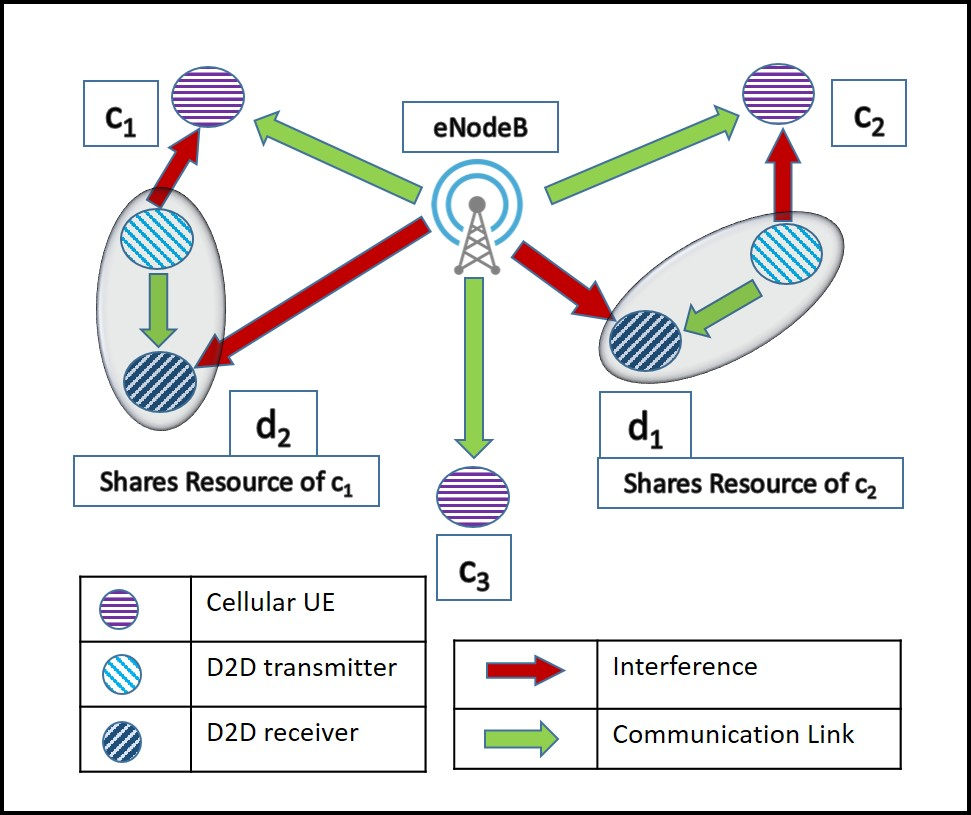
\includegraphics[width=70mm, height=55mm]{Graph/SystemModel.jpg}
		\caption{System Model Using Downlink Resources} \label{fig:system_model}
	}
\end{figure}

%\begin{figure*}[t]
%	{%
%		\setlength{\fboxsep}{1.5pt}%
%		\setlength{\fboxrule}{1.5pt}%
%		\fbox{
%			\begin{subfigure}{0.199\linewidth}
%				\centering
%				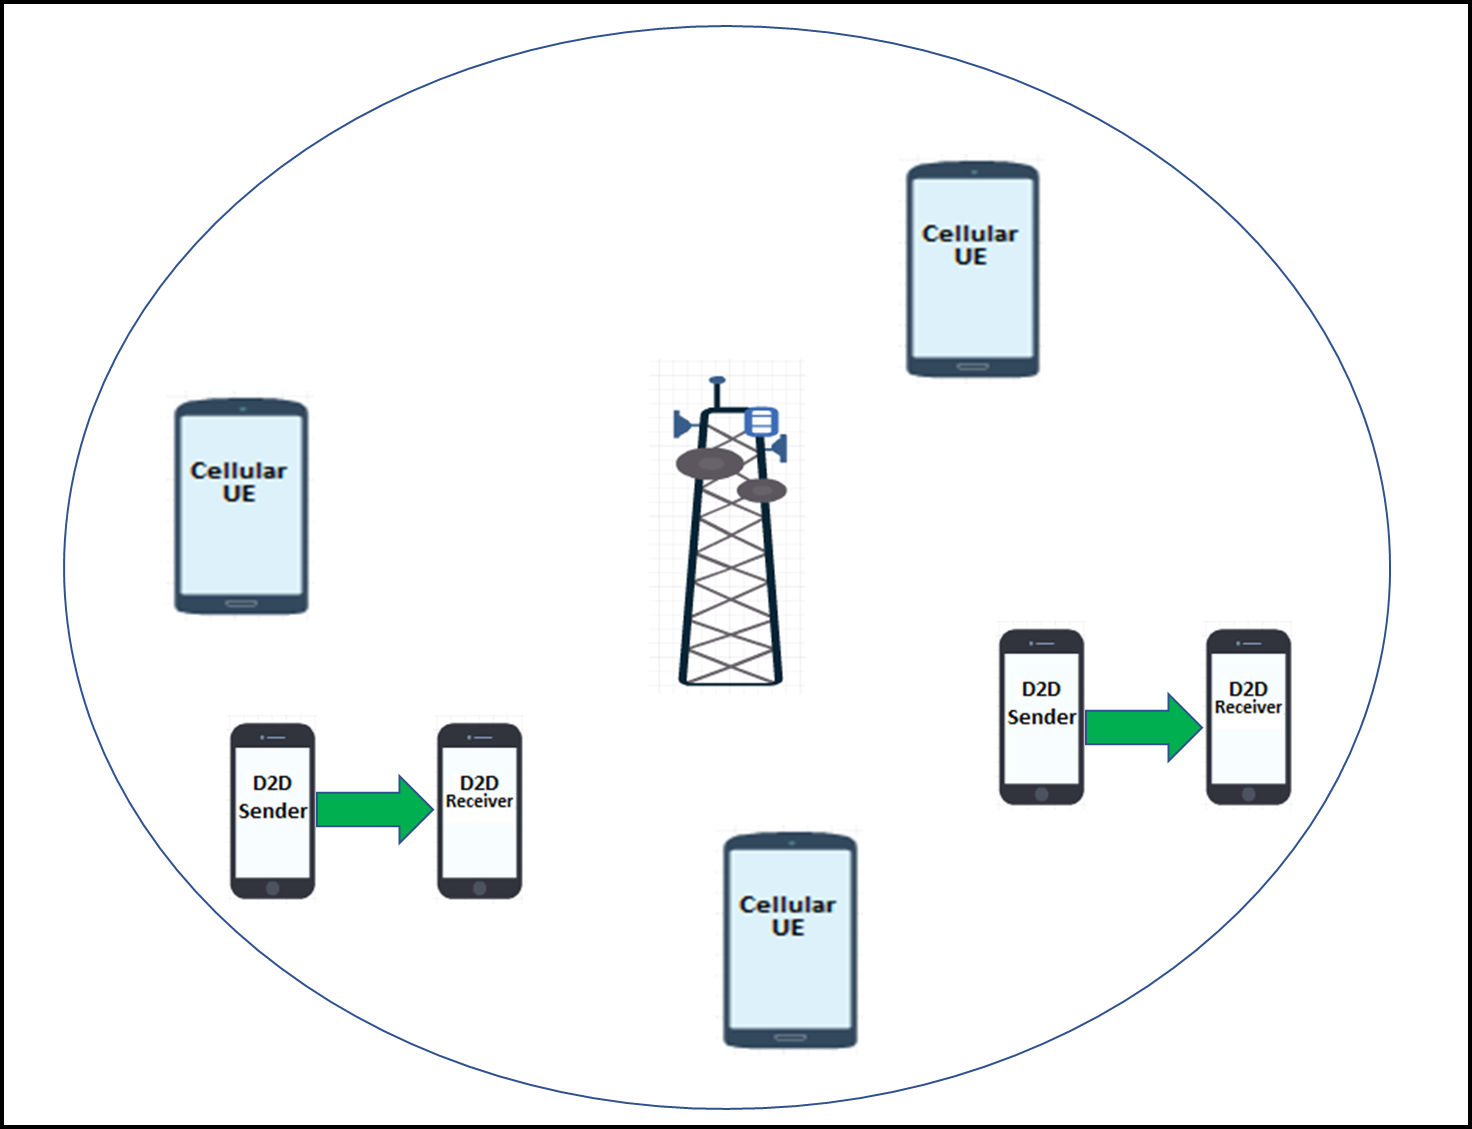
\includegraphics[width=\linewidth]{Graph/s1.png}
%				\caption{Initial State}
%				\label{fig:Initial State}
%			\end{subfigure}
%			\begin{subfigure}{0.199\linewidth}
%				\centering
%				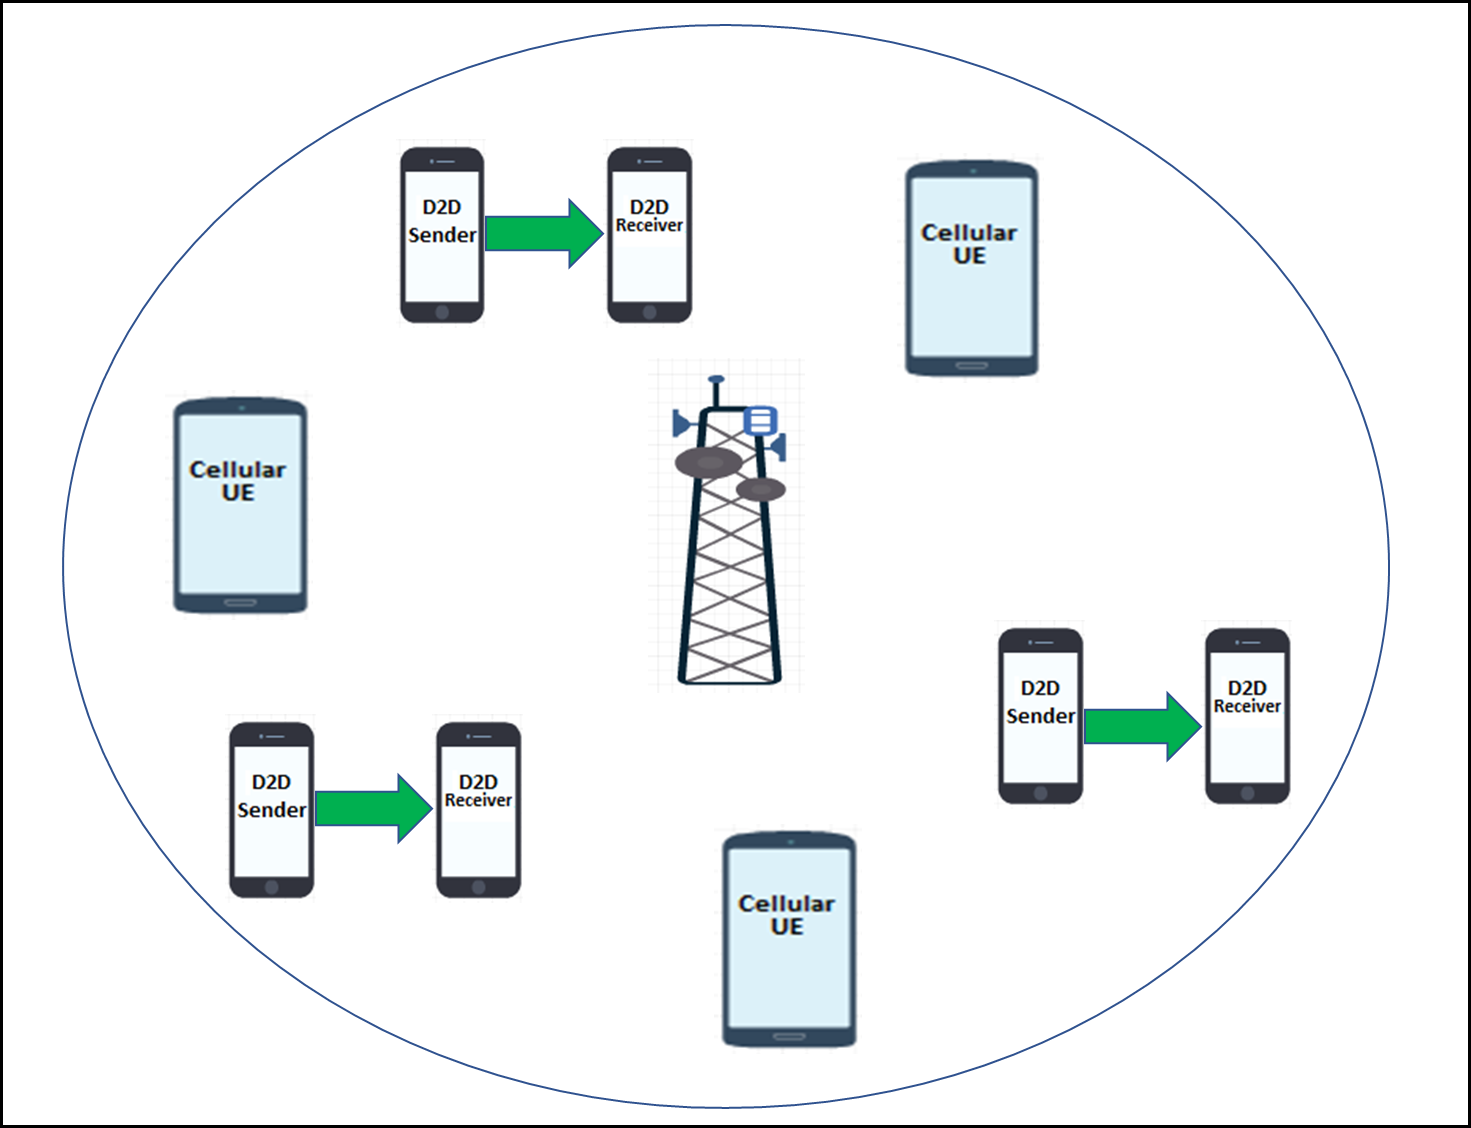
\includegraphics[width=\linewidth]{Graph/s2.png}
%				\caption{D2D Arrival}
%				\label{fig:D2D Arrival}
%			\end{subfigure}
%			\begin{subfigure}{0.199\linewidth}
%				\centering
%				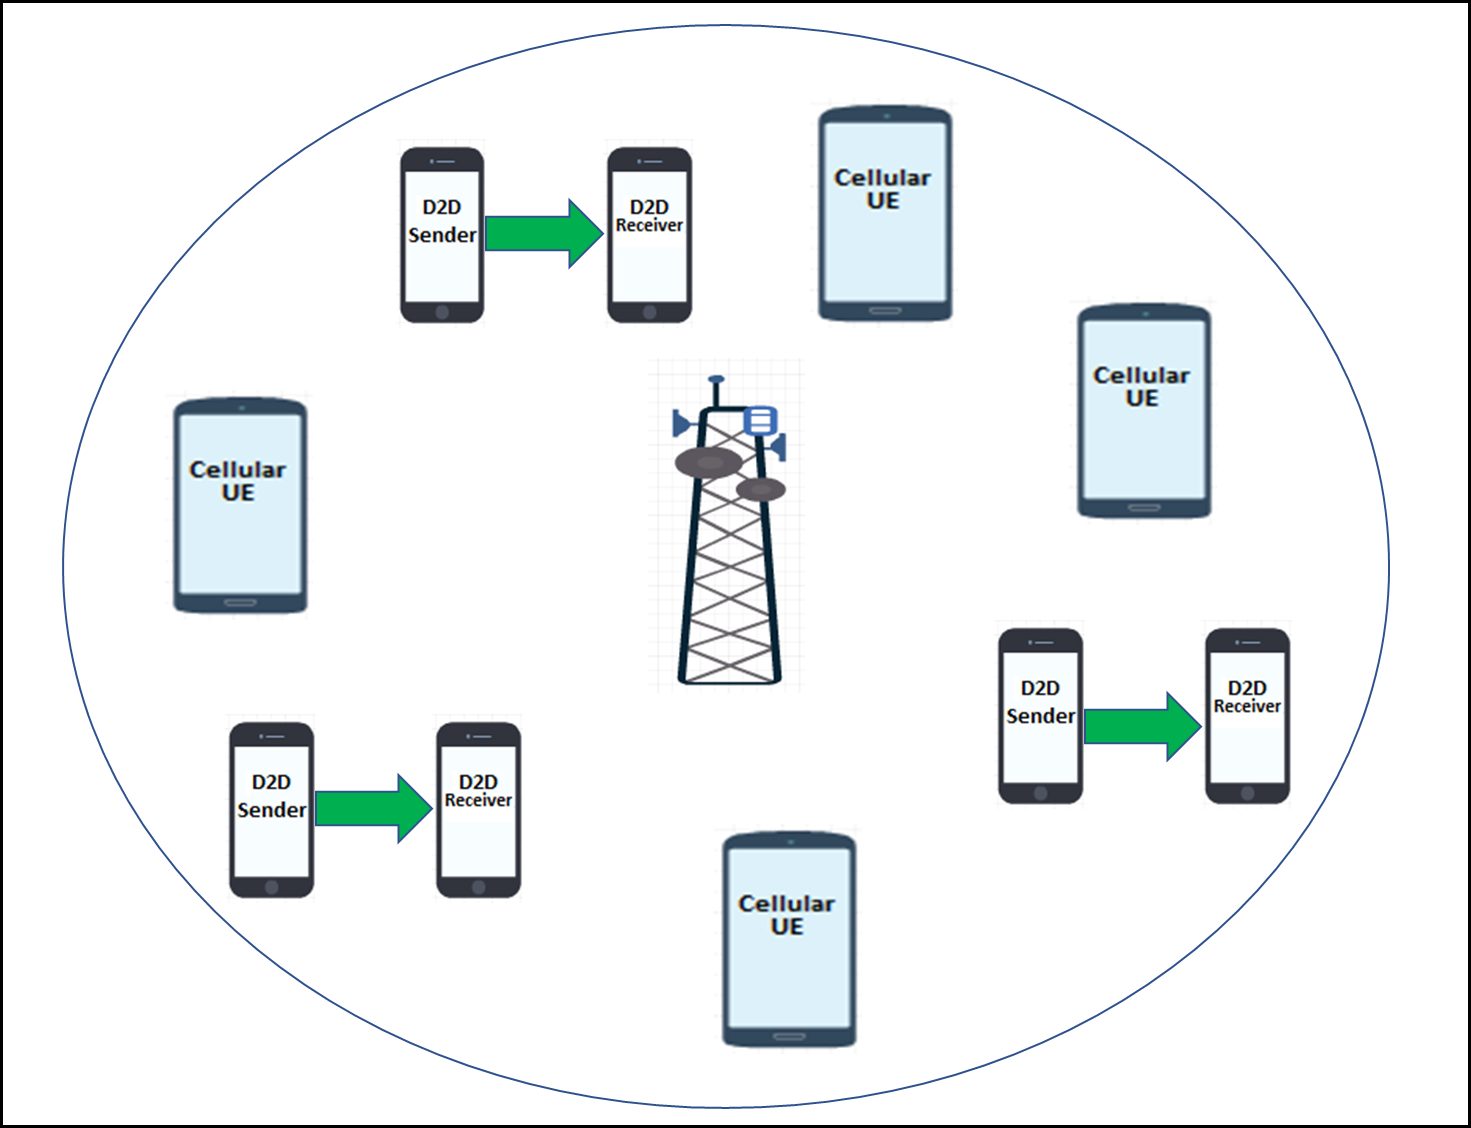
\includegraphics[width=\linewidth]{Graph/s3.png}
%				\caption{Cellular Arrival}
%				\label{fig:Cellular Arrival}
%			\end{subfigure}
%			\begin{subfigure}{0.199\linewidth}
%				\centering
%				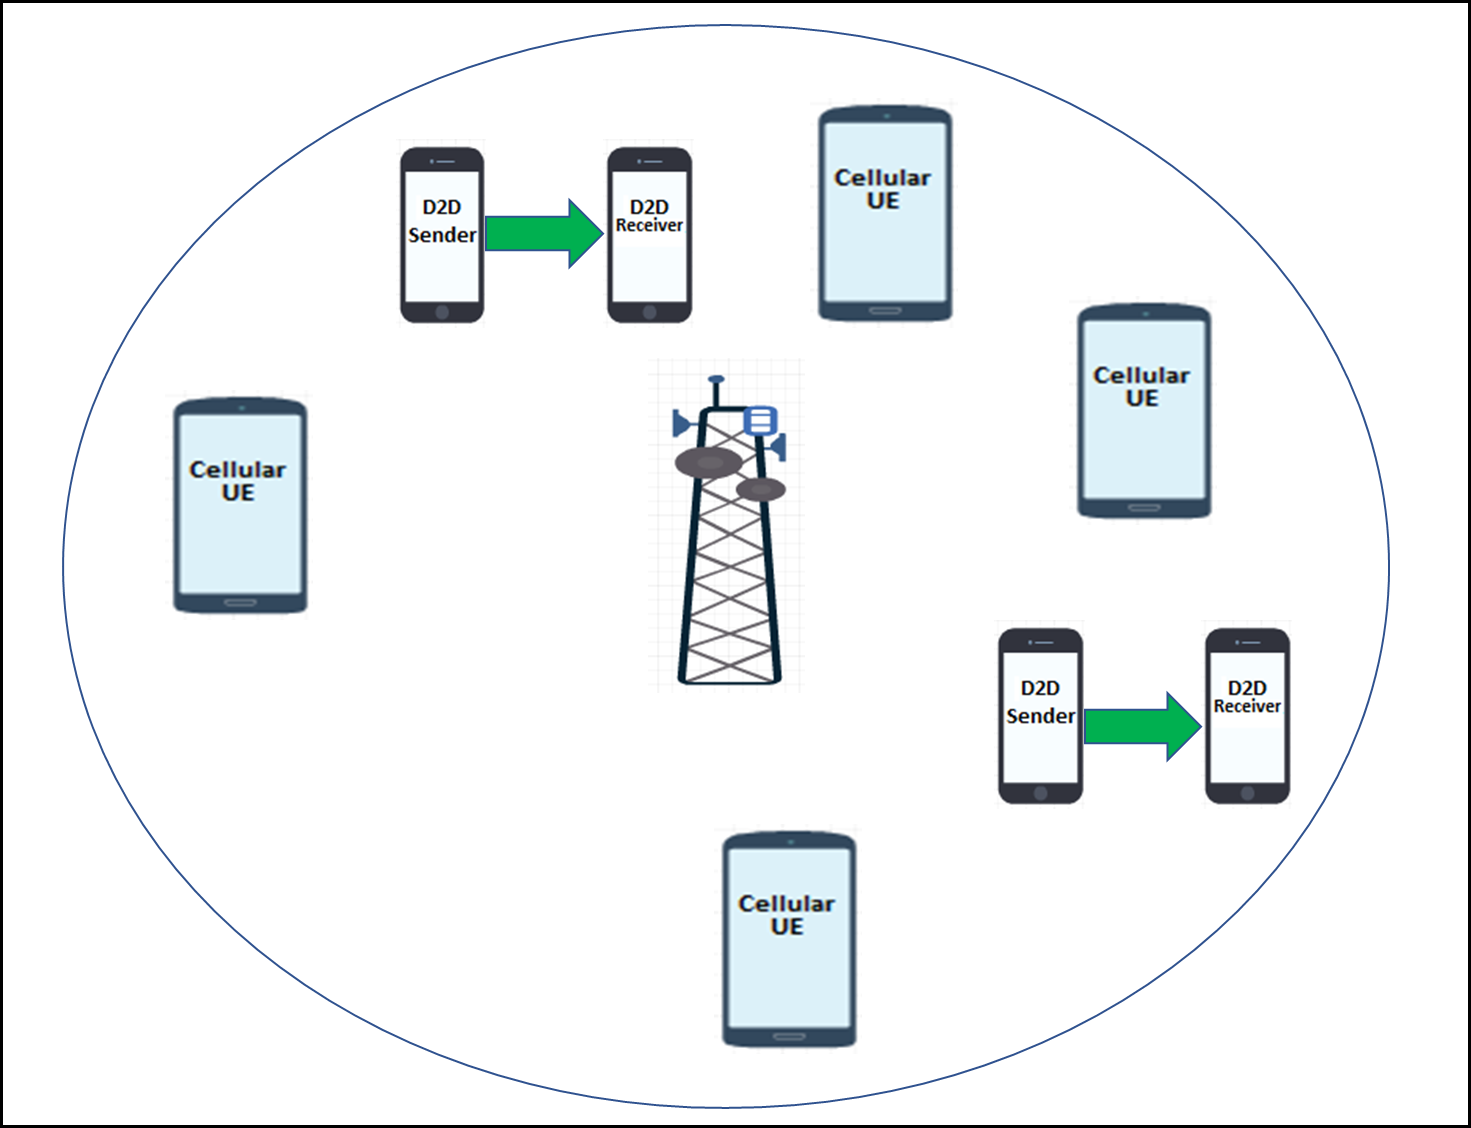
\includegraphics[width=\linewidth]{Graph/s4.png}
%				\caption{D2D Departure}
%				\label{fig:D2D Departure}
%			\end{subfigure}
%			\begin{subfigure}{0.199\linewidth}
%				\centering
%				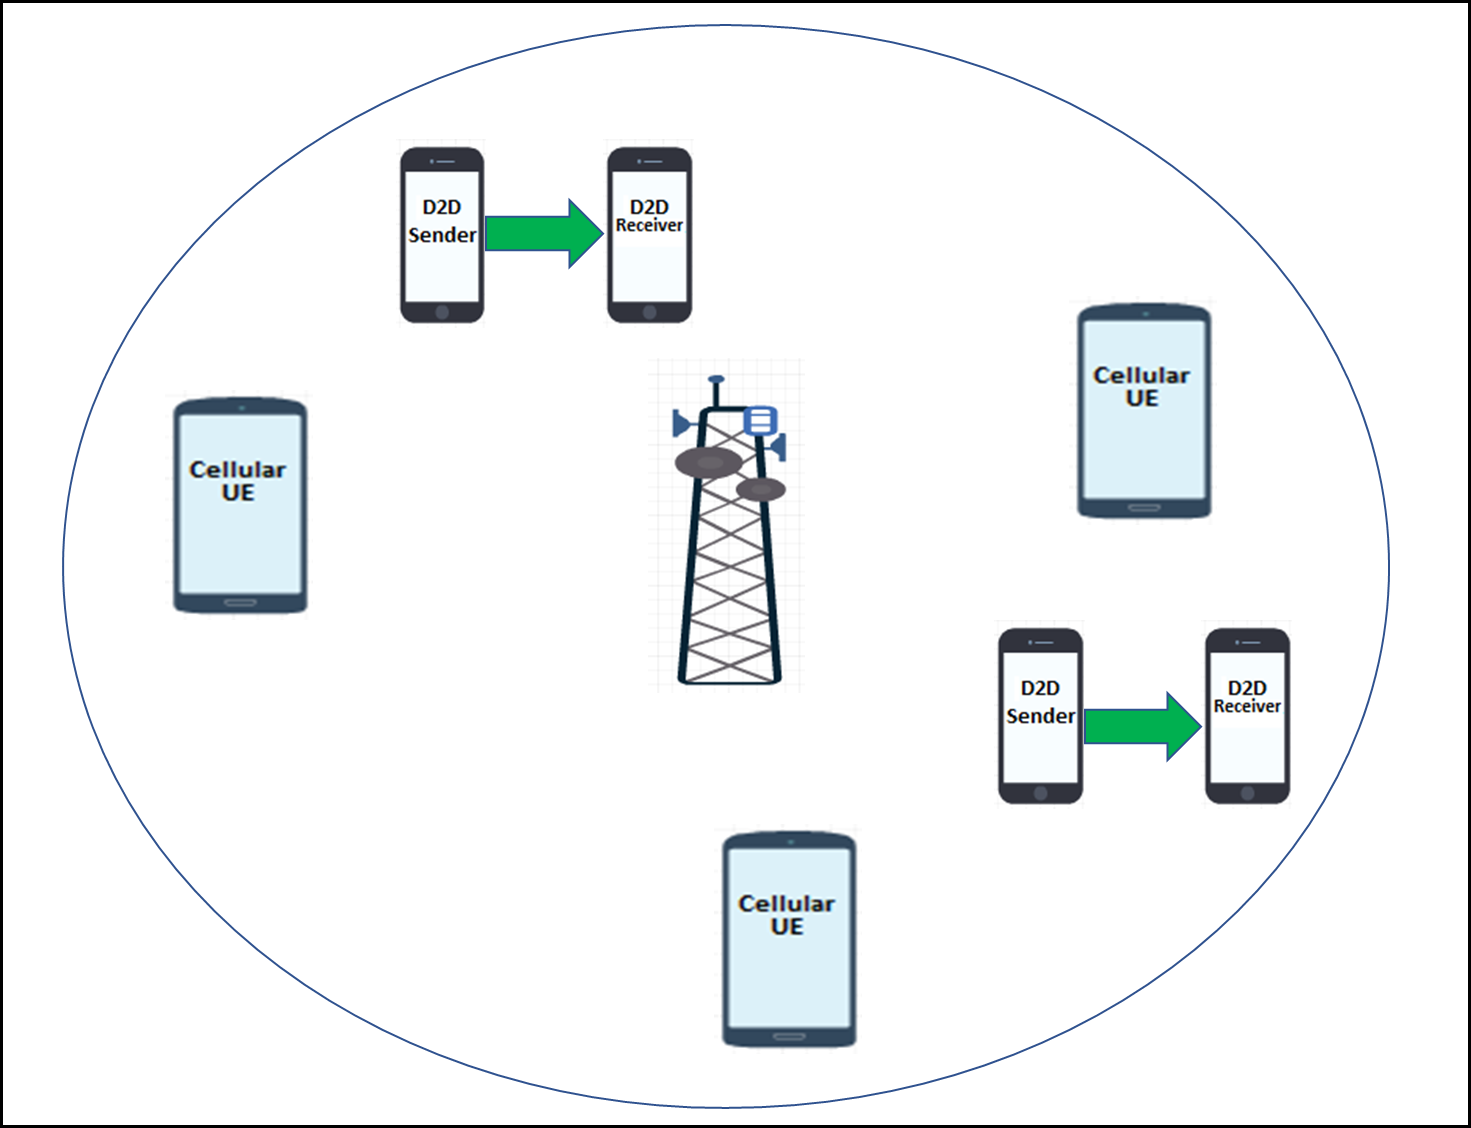
\includegraphics[width=\linewidth]{Graph/s5.png}
%				\caption{Cellular Departure}
%				\label{fig:Cellular Departure}
%			\end{subfigure}
%			
%		}
%	}%
%	\caption{States of the System}
%	\label{fig:State of the System}
%\end{figure*}

\noindent
This paper considers a system with a single cell area consisting of a single eNB, some D2D pairs, and some cellular UEs. 
%(the distributions of the users and D2D pairs are discussed in simulation sections). 
In a normal scenario, total number of the cellular UEs is much higher than the total number of the D2D pairs. We consider the similar scenario used in \cite{lora},\cite{zulhasnine},\cite{dara} with $n$ cellular UEs and $m$ D2D pairs ($n$$>>$$m$) and a cellular UE can share the RBs with a single D2D pair.
The set of the cellular UEs is represented as $C$ = \{$ c_{1}, c_{2}, c_{3}, ..., c_{n} $\},  
whereas the set of the D2D pairs is represented as $D$ = \{$ d_{1}, d_{2}, d_{3}, ..., d_{m} $\}. 
A D2D pair $d_{j} \in D$ contains a receiving device $d_j^r$ and a transmitting device $d_j^t$. Though the D2D pairs directly communicate with each other, the connection establishment and the resource allocation is handled by the eNB \cite{dara}. 

\smallskip
\noindent
LTE network consists of both uplink (UL) and downlink (DL) resources. In our work, we only consider the DL resources  and Figure \ref{fig:system_model} represents the system model we consider. The eNB transmits a signal to the cellular UEs using DL resources, so the cellular UEs only experience interference from their shared D2D transmitters ($c_1$ is affected by $d_2$ and $c_2$ is affected by $d_1$) whereas D2D receivers encounter interference from the eNB (both $d_1$ and $d_2$ are affected by the eNB). As $c_3$ does not share the RBs with any of the D2D pairs, $c_3$ experiences no interference.

\smallskip
\noindent
We consider an Urban Micro System, which follows Rayleigh fading path loss model \cite{lora},\cite{zulhasnine},\cite{dara}. As the channels are assumed to be orthogonal, only intra channel interference is present. The path loss (db unit) equation is 
\begin{equation}
	PL = 36.7\log_{10}(dist)+22.7+26\log_{10}(f_{c}),
\end{equation}
where $dist$ (meter) is the distance between a D2D transmitter and a receiver and $f_{c}$ (GHz) is the medium frequency.
Now the channel gain between these two devices is 
\begin{equation}
	G^{x,y} = 10^{-PL^{x,y}/10},
\end{equation}
where $x$ and $y$ are the two devices and $PL^{x,y}$ is the distance dependent path loss between $x$ and $y$.
% and $S^{x,y}$ is the small scale fading between x and y.

\smallskip


\noindent
We consider the total number and the relative position of the cellular UEs and the D2D pairs in the system at any moment as a state of the system. The state of the system changes over time due to the arrival or departure of the D2D pairs into the system as well as due to the mobility of both of the cellular UEs and the D2D pairs. Figure \ref{fig:State of the System} depicts different states of the system with the arrival and departure of the D2D pairs. We consider the D2D arrival/departure as a system event that triggers the resource allocation process to allocate the RBs for the new state of the system. In other words, we can say when a new D2D pair arrives into the system, the necessary RBs for communication need to be allocated to the newcomer as this event changes the state of the system. We also accommodate user mobility in our model by defining some decision points where we trigger our resource allocation scheme with the new location of the devices (cellular UEs and D2D pairs). Every decision point is considered as a system event because it represents a new state of the system as the location of the devices are changed. However, we impose restrictions on the minimal interval between two decision points. We limit this just to keep the model simple otherwise implementation of user mobility in our system would be impractical.


\begin{figure*}[t]
	{%
		\setlength{\fboxsep}{1.5pt}%
		\setlength{\fboxrule}{1.5pt}%
		\fbox{
			\begin{subfigure}{0.33\linewidth}
				\centering
				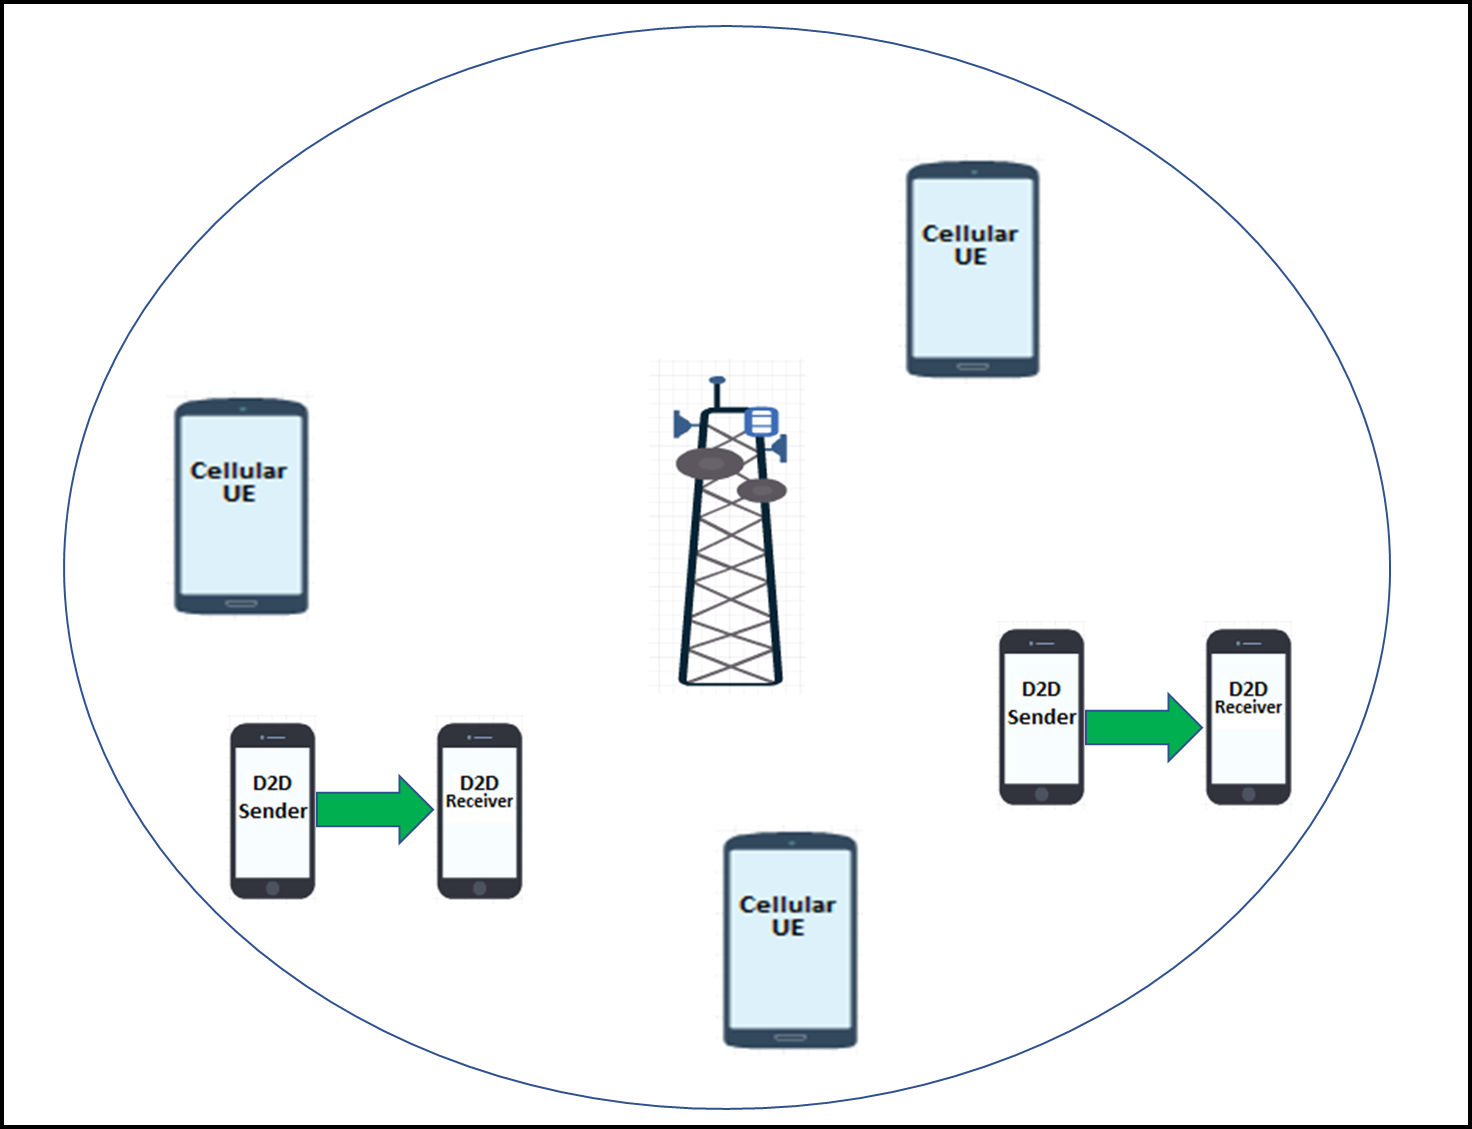
\includegraphics[width=\linewidth]{Graph/s1.png}
				\caption{Initial State}
				\label{fig:Initial state}
			\end{subfigure}
			\begin{subfigure}{0.33\linewidth}
				\centering
				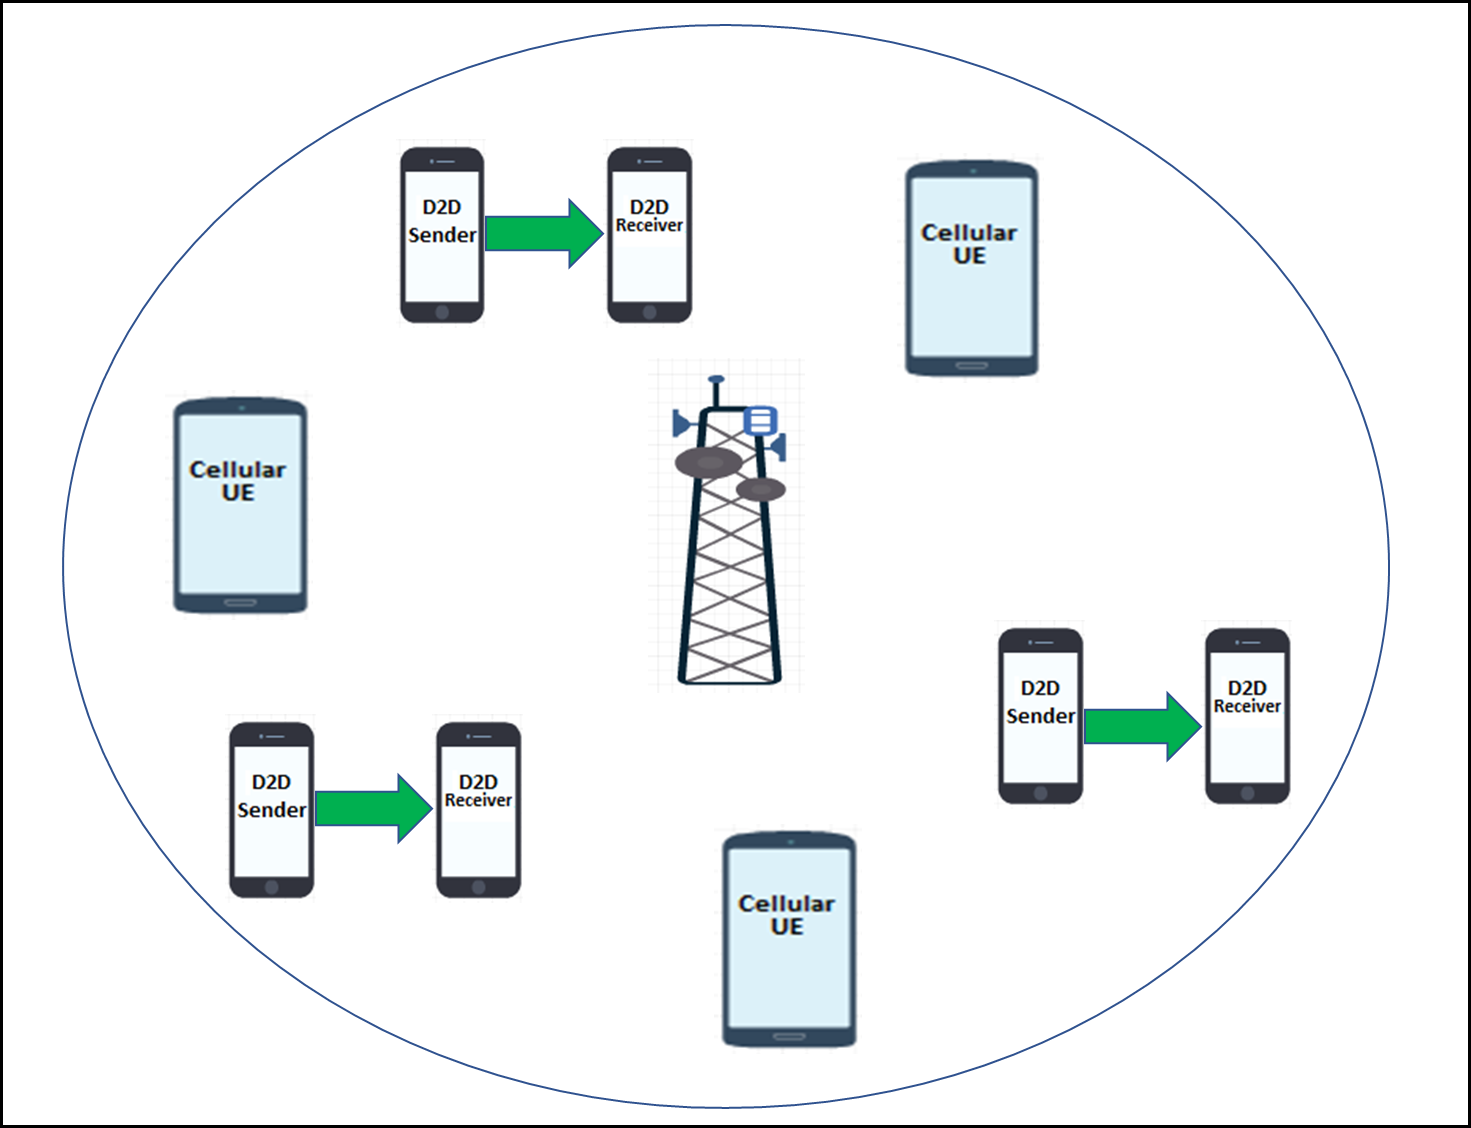
\includegraphics[width=\linewidth]{Graph/s2.png}
				\caption{D2D Arrival}
				\label{fig:D2D arrival}
			\end{subfigure}
%			\begin{subfigure}{0.199\linewidth}
%				\centering
%				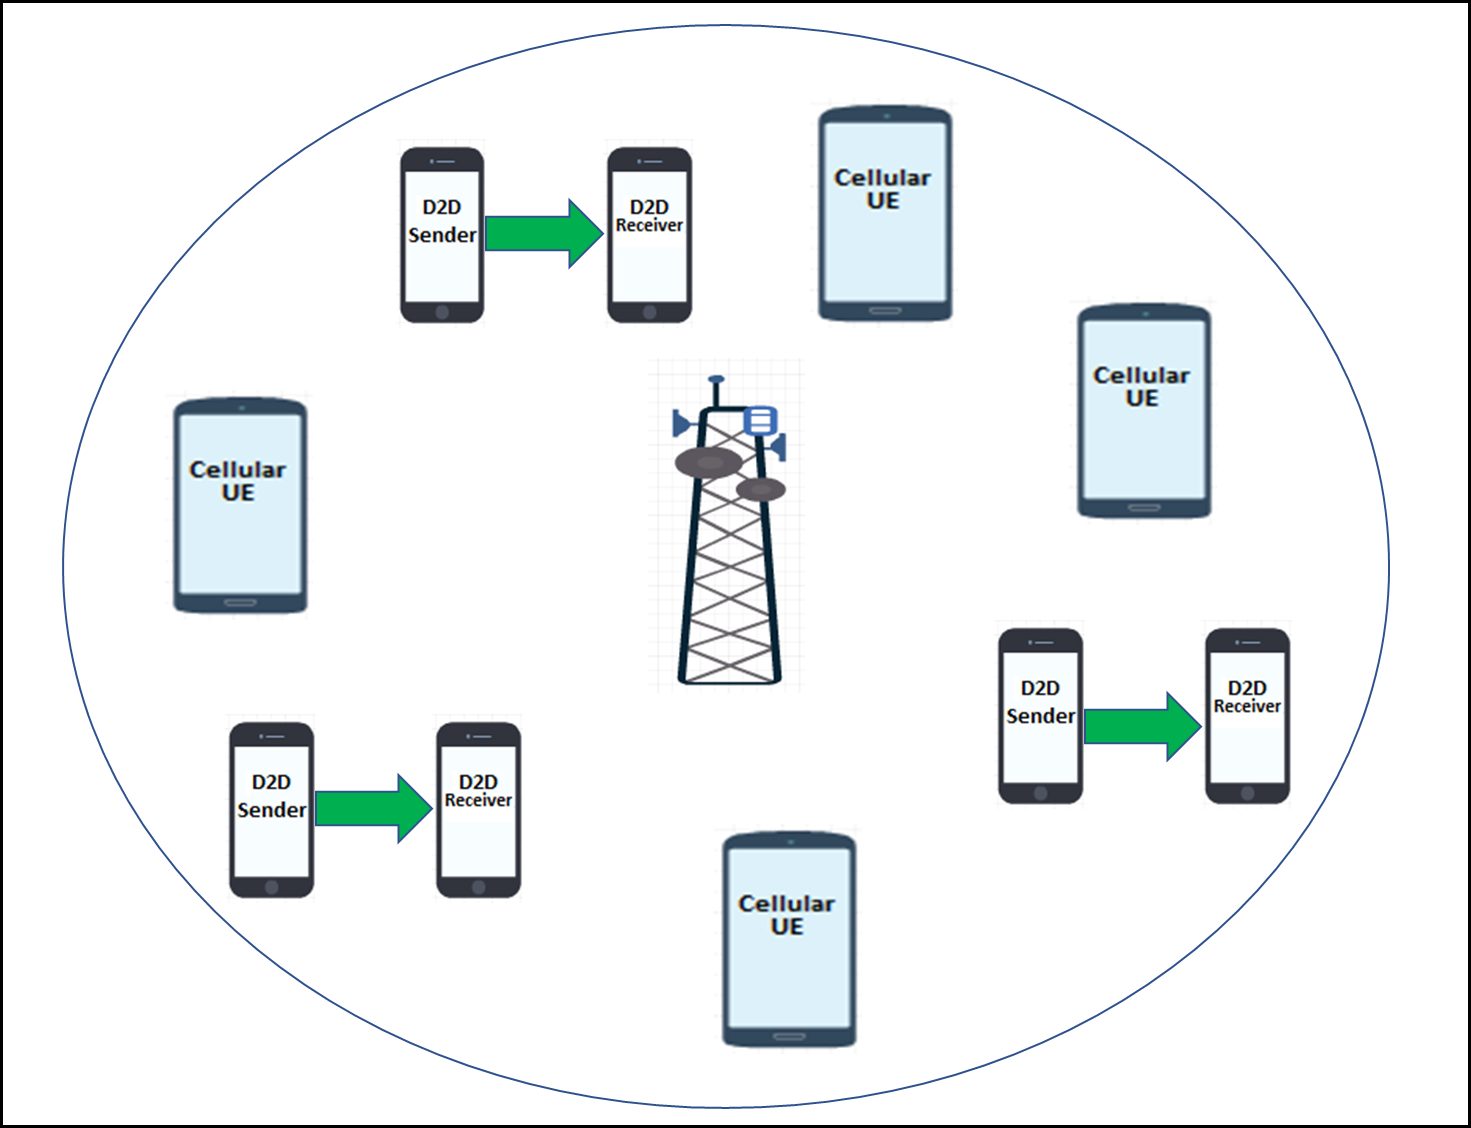
\includegraphics[width=\linewidth]{Graph/s3.png}
%				\caption{Cellular Arrival}
%				\label{fig:Cellular Arrival}
%			\end{subfigure}
			\begin{subfigure}{0.33\linewidth}
				\centering
				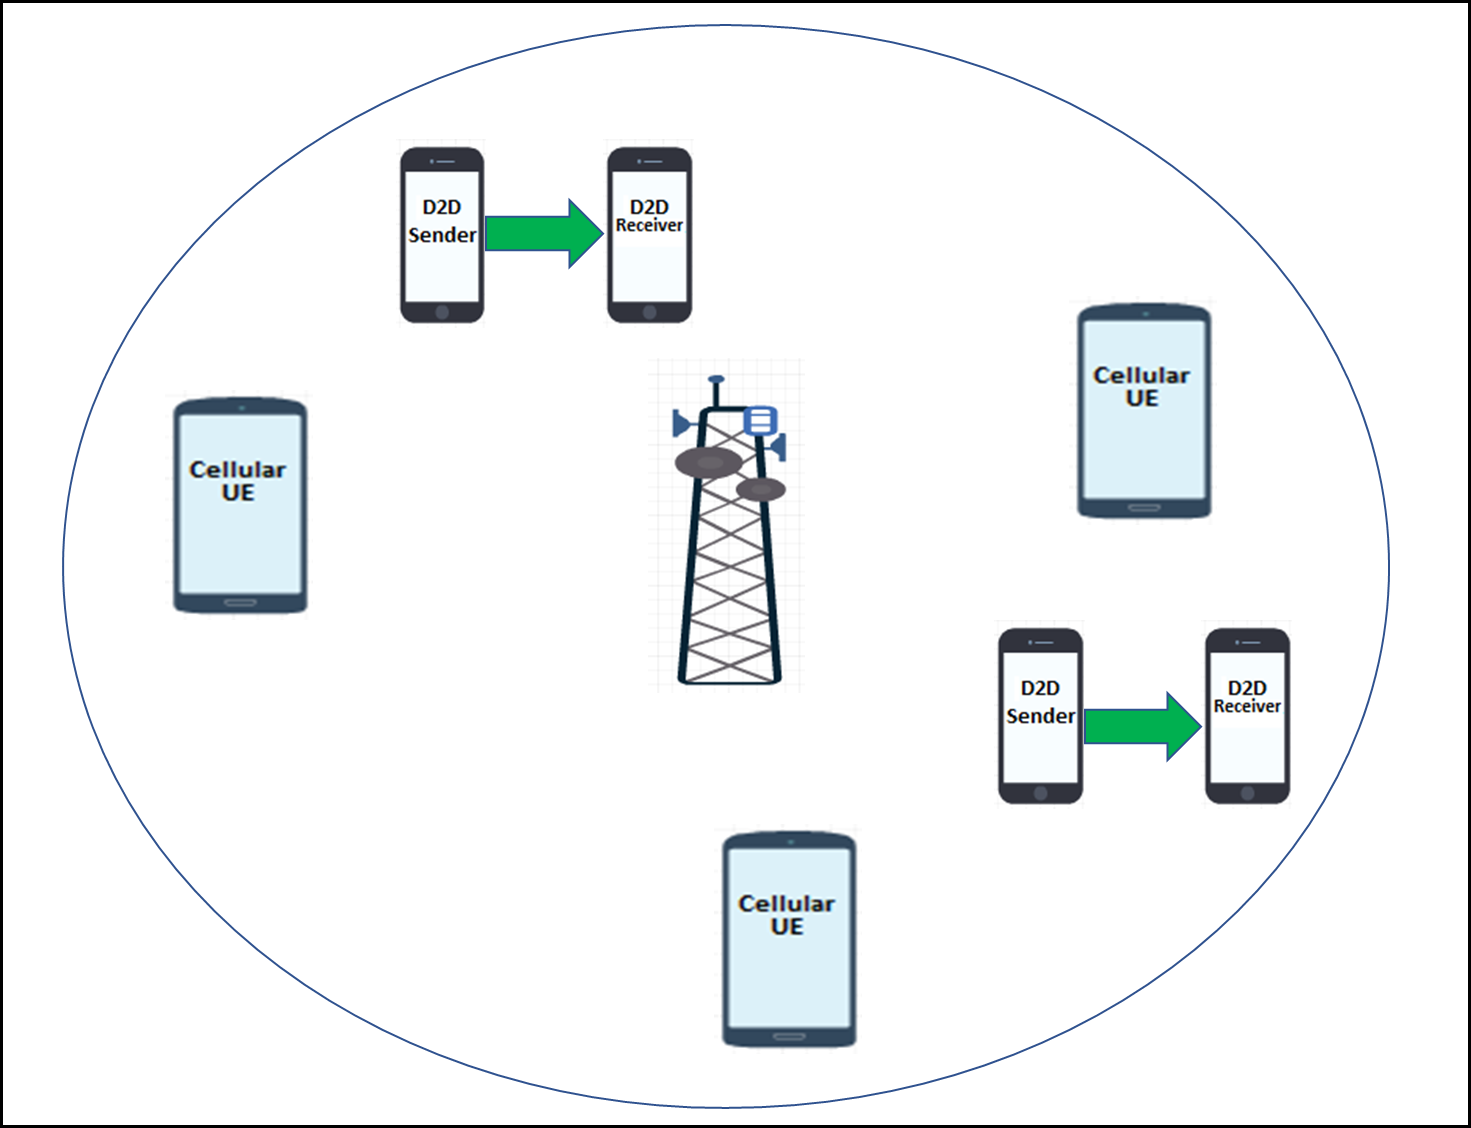
\includegraphics[width=\linewidth]{Graph/s5.png}
				\caption{D2D Departure}
				\label{fig:D2D departure}
			\end{subfigure}
%			\begin{subfigure}{0.199\linewidth}
%				\centering
%				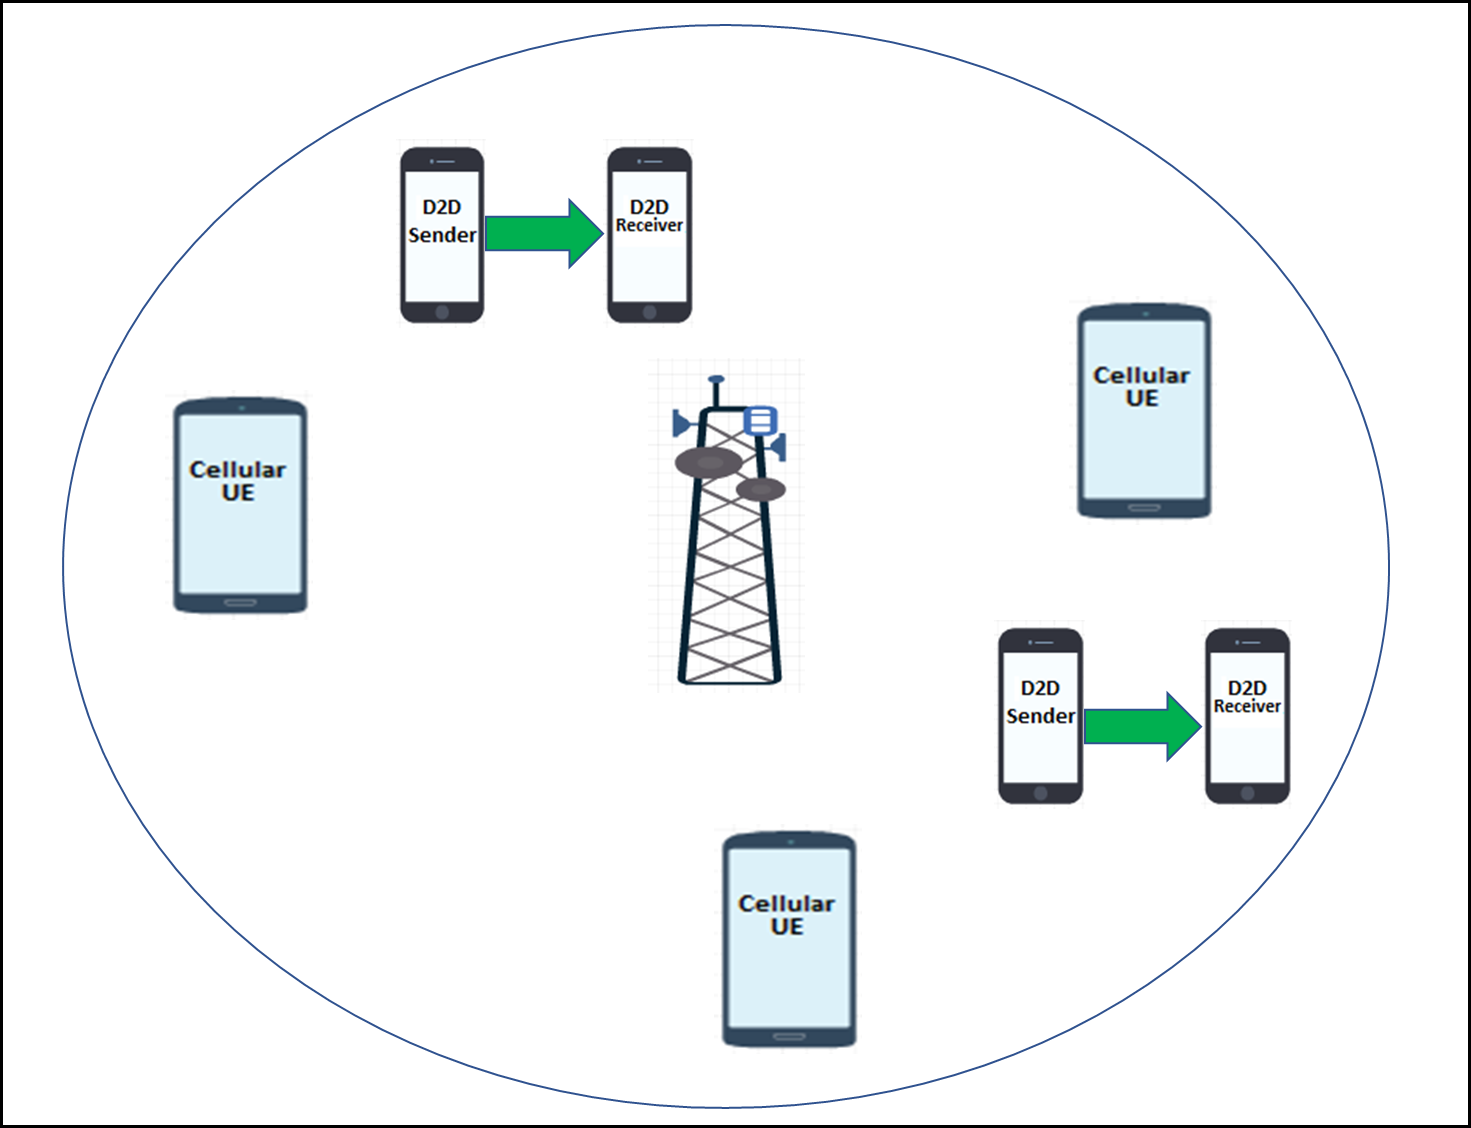
\includegraphics[width=\linewidth]{Graph/s5.png}
%				\caption{Cellular Departure}
%				\label{fig:Cellular Departure}
%			\end{subfigure}
			
		}
	}%
	\vspace{-0.2cm}
	\caption{Different States of the System}
	\label{fig:State of the System}
\end{figure*}  

%Although the relative position of a node is considered to define a state of the system, the user mobility is not considered as a system event to trigger the resource allocation process. We are limiting this just to keep the simulation simple because if user mobility is allowed for the algorithm, all preference lists would need to be completely recalculated at each decision point of mobility which makes the implementation impractical. Moreover, if the user mobility is very frequent then it makes the situation more complex. However, for a relatively stationary system, user mobility might be considered as a system event to trigger the resource allocation process by imposing some restrictions like minimal interval between two consecutive events. This might be a different branch of research to investigate user mobility in online resource allocation.  

%\begin{itemize}
%	\item \textbf{D2D Arrival:} New D2D pair comes in the cell. Resource Blocks need to be allocated to the newcomer. So this event changes the state of the system. 
		  
%	\item \textbf{Cellular Arrival:} A new cellular UE comes in the cell making the previous sharing a sub-optimal solution. There is a chance that sharing may change to attain higher sumrate consequently changes the state of the system.
	
%	\item \textbf{D2D Departure:} A D2D pair leaves the system making the previous sharing a sub-optimal solution. There is a possibility that existing D2D pair can share with the newly freed cellular UE to attain a higher system sumrate.
	
%	\item \textbf{Cellular Departure:} If a shared cellular UE leaves the system then the shared D2D pair will be out of resource blocks. Thus the system state is changed.  
%\end{itemize} 

%These events are represented in the figure \ref{fig:State of the System}.




%\section{Input Data Model}


\section{Problem Formulation}\label{section:Problem Formulation}
%\vspace{-0.5cm}
\vspace {-0.3cm}
\noindent
The SINR of a receiver is the ratio between the received signal power and the interference with the noise power. In a downlink interference model, the SINR value of a cellular UE depends on the transmitting power of the eNB, channel gain between the eNB and the cellular UE as well as the intra channel interference. Let us consider the individual transmitting power of the eNB, a cellular UE $c_i$ and a D2D transmitter $d_j^t$ are $P^{eNB}$, $P^{c_i}$ and $P^{d_j^t}$ respectively. The thermal noise which is also known as the energy of Additive White Gaussian Noise introduced at the receiver end is denoted by $\sigma$. So the SINR of a cellular UE $c_i$ in DL phase \cite{zulhasnine} can be represented as


 \begin{equation}\label{eqn:sinr_c}
	\gamma_{c_i}^{DL} = \frac{P^{eNB}G^{eNB,c_i}}{\sigma + \sum_{d_j} x_{c_i}^{d_j}P^{d_j^t}G^{d_j^t,c_i}},
 \end{equation}
 
\smallskip
\noindent
where $G^{d_j^t,c_i}$ implies the channel gain between a D2D transmitter $d_j^t$ and a cellular UE $c_i$. A binary variable $x_{c_i}^{d_j}$ indicates whether the D2D pair $d_j$  shares the RBs of the cellular UE $c_i$ or not. In the denominator, summation refers to the total interference of all the D2D pairs sharing the RBs of the cellular UE $c$.   
If none of the D2D pairs share the RBs of the cellular UE $c_i$, no intra cell interference is incurred. So the SINR of such the cellular UE using DL resources can be represented as
 \begin{equation}\label{eqn:sinr_c0}
 \gamma_{c_i^0}^{DL} = \frac{P^{eNB}G^{eNB,c_i}}{\sigma}.
 \end{equation}
\noindent 
Similarly, the SINR at the receiving end of a D2D pair $d_j$ using DL resources \cite{zulhasnine} can be presented as
\begin{equation}\label{eqn:sinr_d}
 \gamma_{d_j}^{DL} = \frac{\sum_{c_i} x_{c_i}^{d_j}P^{d_j^t}G^{{d_j^t},d_j^r}}{\sigma + P^{ eNB}G^{ eNB,d_j^r}},
\end{equation}
where $G^{d_j^t,d_j^r}$ implies the channel gain between the transmitting end $d_j^t$ and the receiving end $d_j^r$ of the D2D pair $d_j$. Summation on the numerator indicates the total signals incurred from a D2D pair $d_j$ for different cellular UEs sharing the same D2D pair $d_j$.

\smallskip
\noindent
If $B$ is the channel bandwidth then according to the Shannon's Capacity formula, the sumrate contribution of a cellular UE $c_i$ using DL resources can be presented as

\begin{equation}\label{eqn:sumrate_c}
	R_{c_i}^{DL} = B\log_{2}(1+\gamma_{c_i}^{DL}).
\end{equation}

\noindent
If none of the D2D pairs share the RBs of the cellular UE $c_i$, then the sumrate contribution of $c_i$ can be presented as

\begin{equation}\label{eqn:sumrate_c0}
	R_{c_i^0}^{DL} = B\log_{2}(1+\gamma_{c_i^0}^{DL}).
\end{equation}


\noindent
Similarly, the sumrate contribution of the D2D pair $d_j$ using DL resources can be presented as

\begin{equation}\label{eqn:sumrate_d}
	R_{d_j}^{DL} = B\log_{2}(1+\gamma_{d_j}^{DL}).
\end{equation}
%\noindent
%where we can replace the value of $p$ with $(c_i,d_j)$, $(c_i,0)$ and $(d_j,c_i)$ to get the sum rate of a shared cellular UE (A D2D pair $d_j$ shares the RBs of the cellular UE $c_i$), a free cellular UE (none of the D2D pairs shares the RBs of the cellular UE $c_i$) and a D2D pair $d_j$ (provided that $d_j$ is using the RBs of cellular UE $c_i$) respectively. For later references we represent the sumrate contribution of a cellular UE $c_i$ in the DL phase as a decision variable $R_{c_i}^{DL}$  such that,
%
%	\[ R_{c_i}^{DL} = \left\{ \begin{array}{ll}
%         R_{c_i,d_j}^{DL}, & \mbox{if resources of cellular UE $c_i$ is shared by $d_j$,}\\
%         R_{c_i,o}^{DL}, & \mbox{otherwise}.\end{array} \right. \]  

\noindent
Now based on Eqn.~(\ref{eqn:sumrate_c}), Eqn.~(\ref{eqn:sumrate_c0}) and Eqn.~(\ref{eqn:sumrate_d}) the optimization problem of maximizing the total system sumrate while satisfying the QoS requirements can be formulated as 

\begin{align}
&\max \; \Big(\, \sum_{c_i}^{C} (1-\sum_{d_j}^{D}x_{c_i}^{d_j}) R_{c_i^0}^{DL}N_{c_i} + \sum_{c_i}^{C}\sum_{d_j}^{D} x_{c_i}^{d_j}(R_{c_i}^{DL} +  R_{d_j}^{DL})N_{c_i} \, \Big) \label{eqn:objective} \\
\text{sub}&\text{ject}\text{ to,}\notag\\
&\gamma_{c_i}^{DL} \geqslant \gamma_{c_i,target}^{DL}, \: \forall \:c_i\in C \label{eqn:constraintC} \\
&\gamma_{d_j}^{DL} \geqslant \gamma_{d_j,target}^{DL}, \: \forall \:d_j\in D \label{eqn:constraintD}\\
&\sum_{d_j} x_{c_i}^{d_j} \leqslant 1\;,\quad \forall \;c_i \in C \label{eqn:constraintxc}\\
&\sum_{c_i} x_{c_i}^{d_j} \leqslant 1\;,\quad \forall \;d_j \in D \label{eqn:constraintxd}\\
&x_{c_i}^{d_j} = \{0,1\}\;,  		 \quad \forall \;c_i \in C \quad  \text{and} \quad \forall \;d_j \in D, \label{eqn:constraintx}
\end{align}

\noindent
where $x_{c_i}^{d_j}$ is a decision variable which indicates whether a D2D pair $d_j$  shares the RBs of a cellular UE $c_i$ or not and $N_{c_i}$ implies the number of RBs allocated to a cellular UE $c_i$. The first part of the objective function (Eqn.~\ref{eqn:objective}) maximizes the total sumrate contribution of the unassigned cellular UEs where the optimization variable $R_{c_i^0}^{DL}$ represents the sumrate contribution of an unassigned cellular UE $c_i^0$. The second part of the objective function maximizes the total summrate contribution of the assigned cellular UEs with the D2D pairs where the optimization variables  $R_{c_i}^{DL}$ and $R_{d_j}^{DL}$ represent the individual sumrate contributions of a cellular UE $c_i$ and a D2D pair $d_j$ respectively when $d_j$ reuses the RBs of $c_i$. $\gamma_{c_i,target}^{DL}$ and $\gamma_{d_j,target}^{DL}$ represent the SINR thresholds for a cellular UE $c_i$ and a D2D pair $d_j$ respectively. Constraints (\ref{eqn:constraintC}) and (\ref{eqn:constraintD}) ensure the QoS requirements by maintaining a minimum required SINR value for normal transmission rate. Constraint (\ref{eqn:constraintxc}) implies that a cellular UE might share the RBs with a maximum of one D2D pair and constraint (\ref{eqn:constraintxd}) indicates that a D2D pair might share the RBs of a maximum of one cellular UE. Both of the constraints (\ref{eqn:constraintxc}) and (\ref{eqn:constraintxd}) ensure the orthogonality among the cellular UEs and the D2D pairs while sharing the RBs. Finally constraint (\ref{eqn:constraintx}) confirms that the decision variable $x_{c_i}^{d_j}$ is a binary variable. 

\smallskip
\noindent
Although Eqn.~(\ref{eqn:sinr_c}) and Eqn.~(\ref{eqn:sinr_d}) suggest the concept of multiple sharing among the D2D pairs and the cellular UEs, our proposed algorithms avoid multiple sharing among them. As sharing the RBs of a single cellular UE with multiple D2D pairs generate higher interference to the existing cellular network which might not be acceptable and sharing the RBs of multiple cellular UEs by a single D2D pair produces a complex model. However, these constraints are presented here to reflect the general idea. So the stated optimization problem is to maximize the total system sumrate (Eqn.~(\ref{eqn:objective})) while satisfying the constraints (\ref{eqn:constraintC}) - (\ref{eqn:constraintx}).  
%constraints (\ref{eqn:constraintC}), (\ref{eqn:constraintD}), (\ref{eqn:constraintxc}), (\ref{eqn:constraintxd}),  (\ref{eqn:constraintx}). 

\smallskip
\noindent
We define two types of assignment schemes i.e., the restricted assignment scheme and the fair assignment scheme of our proposed solution. In the restricted assignment scheme, if an assignment returns a negative sumrate gain for a particular cellular UE and a D2D pair then that particular sharing is avoided. More specifically, for a cellular UE $c_i \in C$ and a D2D pair $d_j \in D$ if the value of ($R_{c_i}^{DL}$ + $R_{d_j}^{DL}$ - $R_{c_i^0}^{DL}$) is negative then the restricted assignment scheme does not assign the RBs of $c_i$ to $d_j$. However, there is no such restriction on the fair assignment scheme that means every D2D pair gets a fair chance of sharing the RBs of a cellular UE given that constraints (\ref{eqn:constraintC}) and (\ref{eqn:constraintD})) are satisfied. This paper aims to maximize the total system sumrate contributed by all of the individual cellular UEs and the D2D pairs in a particular allocation in both of the fair and the restricted assignment schemes. Moreover, a special attention is given to maintain a minimal number of changes in assignment between two successive states of the system.

\section{Proposed Algorithms}\label{section:Proposed Algorithm}

\noindent
We propose two relax online resource allocation algorithms for D2D communication in inband underlay mode. We name our first algorithm as Relax Online Resource Allocation Algorithm (RORA). Our second algorithm is a variant of our first algorithm and we name our second algorithm as Conservatively Relax Online Resource Allocation Algorithm (CRORA). Both RORA and CRORA are based on stable matching algorithm \cite{knuth1976mariages}. A stable matching algorithm is applied on a bipartite graph of two disjoint sets where all of the members of each set prepare a list that represents their degree of preference for all of the members of another set. To prepare the preference list every member of a set ranks all of the members of another set based on some criteria. The stable matching algorithm finds a matching between two members from two disjoint sets based on the preference list. In other words, we can say a stable matching algorithm maps the elements from one set to the elements of another set. We treat the resource allocation problem as a bipartite matching problem and apply our proposed algorithms to find a stable matching or an assignment between a D2D pair and a cellular UE. The performance of a stable matching algorithm depends on the different criteria based on which preference list is calculated. So before describing our proposed algorithms, we shed some light on the calculation of preference list of any node (D2D pair or cellular UE) in the following subsection.  


%\subsection{Modified existing algorithms}
%\noindent
%We modified some existing online bipartite matching algorithm such a way that it can be used in the proposed problem. As the problem stated above, we treat the problem as a bipartite matching problem. In [], author proposed an online version of bipartite matching problem. The modified versions of the algorithms are discussed in the following subsections:

%\subsubsection{Greedy Online Algorithm (single entry)}
%\noindent
%In this approach at a moment single D2D In event will be handled. No Cellular In event will cause any change in this algorithm. Cellular Out event where the cellular is assigned to any D2D will go through the special process. This  Cellular Out event will be assumed as a new D2D In the event where the D2D will be the previously assigned D2D. 
%\noindent
%When a new D2D will enter into the system then a list of valid unassigned Cellular UE will be calculated. A valid Cellular UE means where sharing of RBs of the cellular UE with the new comer D2D pair will not break the sinr constraint. From this list of valid cellular UE first one will be chosen. 

%\subsubsection{Ranking Online Algorithm (single entry)}
%\noindent
%The handling of input will be similar as the Greedy Online Approach. But the selection of cellular UE will be different.  
%\noindent
%Like before valid cellular UE list will be calculated. In this case the valid cellular UE list will be sorted in descending based on the sumrate contribution of the shared cellular UE and D2D pair. After that the first cellular will be chosen.

%\subsubsection{Stable Matching Algorithm on unshared Cellular UE and D2D pair}
%\noindent
%In this approach after any event we will find out the un-shared cellular UE and D2D pairs. After this stable matching algorithm will be applied to this set of cellular UEs and D2D pairs.

%\subsubsection{Hungarian algorithm on unshared Cellular UE and D2D pair}
%\noindent
%In this approach after any event we will find out the un-shared cellular UE and D2D pairs. After this Hungarian algorithm will be applied to this set of cellular UEs and D2D pairs.


\subsection{Weight based Preference List} \label{preference list}


\noindent
Preference list of a node of a bipartite graph is the main element of a stable matching algorithm. Existing stable matching based algorithm \cite{dara} for resource allocation in D2D communication uses proximity as the basis of preference list calculation where a node with a lower distance is preferred over a node with a higher distance. In our proposed algorithms, instead of using the proximity we use sumrate gain as a  weight value to generate the preference list of a node. As our prime goal is to maximize the total system sumrate, so in preference calculation, sumrate gain is the weight value. 

\smallskip

\noindent
Assume that, $R_{c_i}^{d_j}$ is the sumrate contribution when a cellular UE $c_i$ shares the RBs with a D2D pair $d_j$ and $R_{c_i}^{0}$ is the sumrate contribution when the cellular UE $c_i$ does not share the RBs with any of the D2D pairs. So,



\begin{equation}
	\triangle R = R_{c_i}^{d_j}-R_{c_i}^{0} \label{eqn:sum rate increment}
\end{equation}  
       
    

\noindent
implies the gain in total system sumrate when a cellular UE $c_i$ shares the RBs with a D2D pair $d_j$. So if the value of $\triangle R$ is nonnegative then that particular sharing does not reduce the total system capacity. So, $\triangle R$ is the weight based on which the preference lists of all of the nodes are calculated. In our proposed algorithms, a D2D pair $d_j$ prefers a cellular UE $c_i$ over another cellular UE $c'_i$ if ($c_i$,$d_j$) provides better sum rate gain than ($c'_i$,$d_j$) and same thing is true for a cellular UE. The sumrate gain can be either positive or negative that means the total system sumrate can either increase or decrease if a D2D pair shares the RBs of a cellular UE. We define a binary variable $p_{c_i,d_j}^{R}$ to indicate the presence of a node (cellular UE or D2D pair) in the preference list of another node for the restricted scheme as

\[ p_{c_i,d_j}^{R} = \left\{ \begin{array}{ll}
         1, & \mbox{if $\triangle R$ is non-negative and constraints ($\ref{eqn:constraintC}$) and ($\ref{eqn:constraintD}$) are satisfied,}\\
         0, & \mbox{otherwise}.\end{array} \right. \]

\noindent         
which indicates that in the case of the restricted assignment scheme if a D2D pair $d_j$ and cellular UE $c_i$ return non-negative sumrate gain and satisfy constraints ($\ref{eqn:constraintC}$) and ($\ref{eqn:constraintD}$) then only  $d_j$ is kept in the preference list of $c_i$ and vice-versa.        
\noindent
In the case of the fair assignment scheme, all of the nodes are always kept in the preference list whether they are providing positive or negative sumrate gain given that constraints ($\ref{eqn:constraintC}$) and ($\ref{eqn:constraintD}$) are satisfied. Similarly for the fair assignment scheme we define a binary variable $p_{c_i,d_j}^{F}$ as  

\[ p_{c_i,d_j}^{F} = \left\{ \begin{array}{ll}
         1, & \mbox{if constraints  ($\ref{eqn:constraintC}$) and ($\ref{eqn:constraintD}$) are satisfied,}\\
         0, & \mbox{otherwise}.\end{array} \right. \]  
 

\smallskip


\subsection{Algorithm Scheduler}
\smallskip
\noindent
Algorithm \ref{algorthm1} is a scheduler that triggers our proposed algorithms RORA (Algorithm \ref{algorthm2}) and CRORA (Algorithm \ref{algorthm3}) based on two system events namely arrival event and mobility event. We define the arrival of a D2D pair in the system as an arrival event and the movement of the cellular UEs and the D2D pairs as mobility event. The occurrence of any one or both of the events trigger our proposed algorithms (RORA and CRORA) to give a new assignment for the new state. To accommodate the mobility of the nodes in our proposed solution we define some decision points where we calculate the location of the devices (cellular UEs and D2D pairs). In every decision point, mobility event triggers both of our proposed algorithms because every decision points represent the new state of the system as the location of the devices are changed. In the current implementation, we do not consider the departure event of the D2D pairs to keep the model simple. Although departure event would make the system more realistic its exclusion does not add any demerit point to our proposed algorithms as any of the arrival and departure event would trigger our proposed algorithms (RORA and CRORA) with a new set of cellular UEs and D2D pairs.


\subsection{Relax Online Resource Allocation Algorithm (RORA)}

\medskip
\noindent
Our first proposed algorithm RORA (Algorithm \ref{algorthm2}) is based on the stable matching algorithm \cite{knuth1976mariages} that assumes the cellular UEs as a fixed set and the D2D pairs as an adversary set that means the total number of the D2D pairs varies in the system in course of time. In Algorithm \ref{algorthm2}, we consider the resource allocation problem as a bipartite graph with $n$ cellular UEs in one set and $m$ D2D pairs in another set. At the beginning, we initialize the newly arrived D2D pairs and the unassigned cellular UEs as free (Line $2$ Algorithm \ref{algorthm2}). 
Then we calculate the preference lists for both of the cellular UEs and the D2D pairs based on Eqn.~(\ref{eqn:sum rate increment}) and the binary variables $p_{c_i,d_j}^{R}$ and $p_{c_i,d_j}^{F}$ as described in subsection \ref{preference list}       (Line $3$ Algorithm \ref{algorthm2}). In RORA, the D2D pairs facilitate the proposal part of the stable matching algorithm (Line $5$ Algorithm \ref{algorthm2}). RORA (Algorithm \ref{algorthm2}) assigns a cellular UE and a D2D pair together such that there is no other cellular UEs and D2D pairs that would provide better sumrate than their current assignment (Line $4-7$ Algorithm \ref{algorthm2}). If there are no such cellular UE or D2D pair then all of the assignments are stable. If such assignments occur (Line $10$  Algorithm \ref{algorthm2}) then RORA revokes those assignments. Line number $10$ of Algorithm \ref{algorthm2} actually facilitates the relaxation property of RORA which allows the revocation of an existing assignment. The RBs of the revoked cellular UEs are assigned to the newly arrived D2D pairs and the revoked D2D pairs are added to the list of free D2D pairs. When all of the D2D pairs are assigned to the cellular UEs then RORA stops its execution and returns the allocation as the final result. 
 
 
\subsection{Conservatively Relax Online Resource Allocation Algorithm (CRORA)}
 
\noindent
Our second proposed algorithm CRORA (Algorithm \ref{algorthm3}) is a variant of our first proposed algorithm RORA and works in a similar way as RORA works with some extra carefulness. To leverage the extra system overhead due to the relaxation property (revocation of assignment) we design CRORA in a conservative way. Up to line number $10$ of CRORA is similar to that of  RORA where CRORA calculates the preference lists of both of the cellular UEs and the D2D pairs and considers the D2D pairs as the proposer of the stable matching algorithm. CRORA is a conservative variation of RORA as an extra condition is checked (Line $11$   Algorithm \ref{algorthm3} ) at the time of assignment where there is a necessity of revocation. This new condition ensures that if the revoked D2D pair would contribute negative system sumrate gain along with its new partner then this revocation is not allowed. Hence, the number of changes is reduced and at the same time the objective of sumrate maximization is achieved. The new condition (Line $11$  Algorithm \ref{algorthm3}) considers $c_m \in C$ as the next available preferred cellular UE for the associated D2D pair $d_k$. If $c_m$ is empty, i.e. there is no such free cellular UE for $d_k$ then the sumrate contribution $S_{c_m, d_j}$ = 0. As $c_m$ is free, so  $S_{c_m,0}$ represents the sumrate contribution $c_m$ when it does not share the RBs with any of the D2D pairs. In other words, we can say if there is a necessity of revocation (Line $10$ Algorithm \ref{algorthm3}) right away CRORA will not revoke the assignment, rather it will check the new condition (Line $11$ Algorithm \ref{algorthm3}). If the new condition is satisfied only then it revokes the assignment otherwise CRORA go with the existing assignment hence reducing the number of changes in assignment between two successive allocations. 
 
%Let the preference matrix $P$ have $2n \times n$
%elements. Here, n is the number of cellular UEs and we assume $n > m$ where m is the number of D2D pairs.  Each valid row for D2D pairs in the $P$  matrix contains the list of the cellular users in ascending order of their distance to the D2D pair. However, each valid row for cellular UEs contains $m$ valid entries for the list of the D2D pairs in ascending order of their proximity to the cellular UEs and the rest $n − m$ entries are invalid and does not affect the calculation. Similarly, we maintain another list, $Allocation$, with $2n$ elements to contain the current allocation of the items. In this list, $n + m$ items are valid entries and the rest are invalid and will not affect our calculation.  Initially, there is no association among the D2D and cellular users. We describe deferred acceptance based resource allocation algorithm in Algorithm \ref{algorthm1}.
\par
 \begin{algorithm}	
   \caption{Algorithm Scheduler}
   \label{algorthm1}
    \begin{algorithmic}[1]

    \Procedure{Scheduler}{$D(d_1,d_2,\ldots,d_m), C(c_1,c_2,\ldots, c_n)$}
    \Comment{An allocation from C(cellular UEs) to D(D2D pairs)}
        
        \State Call $RAAlgorithm1(D,C)$ for RORA or $RAAlgorithm2(D,C)$ for CRORA
        
        \While{ $TRUE$}   	
        	\If{$Event_{Arrial}$ $||$ $Event_{Mobility}$}
        	\State Call $RAAlgorithm1(D,C)$ for RORA or $RAAlgorithm2(D,C)$ for CRORA
        	\EndIf       	
        \EndWhile
        	
	\EndProcedure

\end{algorithmic}
\end{algorithm}


\par
 \begin{algorithm}	
   \caption{Relax Online Resource Allocation Algorithm (RORA) }
   \label{algorthm2}
    \begin{algorithmic}[1]

    \Procedure{RAAlgorithm1}{$D(d_1,d_2,\ldots,d_m), C(c_1,c_2,\ldots, c_n)$}
    \Comment{An allocation from C(cellular UEs) to D(D2D pairs)}
       \State Newly arrived D2D pairs and the unassigned cellular UEs are initialized as free.  
        \State Calculate the preference lists for the free cellular UEs and the D2D pairs using Eqn.~(\ref{eqn:sum rate increment})
			
		
		\While{$\exists$  free D2D pair $d_j \in D$ who still has a cellular user $c_i \in C$ to request to}
			\State $c_i$ = first cellular user on $d_j$'s preference list to whom $d_j$ has not yet requested
			\If{$c_i$ is free}
				\State $(c_i,d_j)$ become assigned
			\Else
				\State For another D2D pair $d_k \in D$ an assignment $(c_i, d_k)$ already exists 
				\If{$c_i$ prefers $d_j$ to $d_k$}					                                              
					\State $(c_i, d_j)$ become assigned
					\State Add $d_k$ to the list of free D2D pairs.
				\Else
					\State $(c_i, d_k)$ remain assigned
				\EndIf
			\EndIf
		\EndWhile      	
	\EndProcedure

\end{algorithmic}
\end{algorithm}


\par
 \begin{algorithm}	
   \caption{Conservatively Relax Online Resource Allocation Algorithm (CRORA)}
   \label{algorthm3}
    \begin{algorithmic}[1]

    \Procedure{RAAlgorithm2}{$D(d_1,d_2,\ldots,d_m), C(c_1,c_2,\ldots, c_n)$}
    \Comment{An allocation from C(cellular UEs) to D(D2D pairs)}
       \State Newly arrived D2D pairs and unassigned cellular UEs are initialized as free.  
        \State Calculate the preference lists for the free cellular UEs and the D2D pairs using Eqn.~(\ref{eqn:sum rate increment})
			
		
		\While{$\exists$  free D2D pair $d_j \in D$ who still has a cellular user $c_i \in C$ to request to}
			\State $c_i$ = first cellular user on $d_j$'s preference list to whom $d_j$ has not yet requested
			\If{$c_i$ is free}
				\State $(c_i,d_j)$ become assigned
			\Else
				\State For another D2D pair $d_k \in D$ an assignment $(c_i, d_k)$ already exists
				\If{$c_i$ prefers $d_j$ to $d_k$ }
					\If{$S_{c_i,d_j}$ + $S_{c_m,d_k}$ - $S_{c_m,0}$ $>$ $S_{c_i,d_k}$ }           
                      	\Comment {$c_m \in C$ is the next available preferred channel for $d_k$. } 
                     	\State $(c_i,d_j)$ become assigned
                     	\State $(c_m,d_k)$ become assigned                     	
					 \Else
					    \Comment{we are not changing the assignment as it will not improve the global solution.}	
						\State $(c_i, d_k)$ remain assigned
						\EndIf						
 	            \Else
					\State $(c_i, d_k)$ remain assigned
					
				\EndIf
			\EndIf
		\EndWhile      	
	\EndProcedure

\end{algorithmic}
\end{algorithm}


\subsection{Analysis on Assignment Strategy}\label{assighment stragegy}
\smallskip
\noindent 
In this subsection, we focus on the the assignment strategy of the optimal Hungarian and our proposed algorithms. Here, we present a simple example  (Figure \ref{fig:Number of changes in assignment}) that explains why our proposed algorithms in general needs less number of changes in assignment between two successive allocations compared to the Hungarian algorithm which provides the optimal result in term of total system sumrate \cite{ccnc}. Let us consider the state of Figure \ref{fig:Initial State_} with two cellular users $ c_{1}, c_{2}$  and one D2D pair $d_{1}$. The sumrate contributions of $d_{1}$ are $S_{c_1,d_1}$ and $(S_{c_1, d_1}-\epsilon)$ when it shares the RBs of $ c_{1}$ and $ c_{2}$ respectively where $\epsilon$ is a very small real number. According to both optimal and our proposed algorithms $d_{1}$ would share the RBs of $c_{1}$ (solid lines  represent a valid assignment). Suppose in the next state a new D2D pair $d_{2}$ enters into the system. The sumrate contributions of $d_{2}$ are $(S_{c_1, d_1}-\epsilon)$ and $(S_{c_1, d_1}-3\epsilon)$ when it shares the RBs of $ c_{1}$ and $ c_{2}$ respectively. Now according to the Hungarian algorithm (Figure \ref{fig:Hungarian}) new associations would be $c_1d_2$ and $c_2d_1$ with a total sumrate contribution of $2(S_{c_1, d_1}-\epsilon)$ and it encounters one change in resource allocation ($d_{1}$ is revoked from $c_{1}$ and $d_{2}$ is assigned to $c_{1}$). However, according to our proposed algorithms (Figure \ref{fig:Proposed Algorithm}) the new associations would be $c_1d_1$ and $c_2d_2$ with a total sumrate contribution of $(2S_{c_1, d_1}-3\epsilon)$. It is noted that our proposed algorithms do not encounter any change in resource allocation hence less system overhead contribution.
%\subsection{Example Scenario} 

\smallskip
\noindent
Now, we present a small example in Figure \ref{fig:trace_analysis} that shows the output traces of the optimal Hungarian algorithm, RORA, and CRORA. We generate the output traces for a simple scenario with a fixed number of $5$ cellular UEs and a variable number of D2D pairs. We start with a single D2D pair and in course of time more D2D pairs arrive in the system online and finally, there are $5$ D2D pairs in the system (all of the algorithms terminates when the total number of D2D pairs exceeds the total number of cellular UEs in the system). Figure \ref{fig:trace_hungarian}, \ref{fig:trace_p1} and  \ref{fig:trace_p2} represent the output trace of the optimal algorithm (Hungarian), RORA and CRORA respectively where individual row represents a state of the system with different number of D2D pairs. For all of the algorithms, total system sumrate and number of changes (revocations) in different states of the system are presented in respective columns of Figure \ref{fig:trace_hungarian}, \ref{fig:trace_p1} and  \ref{fig:trace_p2}. The column index of a D2D pair represents the cellular UE to which it is currently assigned to. In every row, green color represents the newly arrived D2D pair and red color represents the revoked D2D pairs from the previous state. For example, in Figure \ref{fig:trace_hungarian} row number $3$ represents the state of the system with $5$ cellular UEs and $3$ D2D pairs where $d_3$ is the newly arrived D2D pair. For this state Hungarian algorithm returns a total sumrate of $157.935$ with a single change in the assignment where $d_2$ is revoked from $c_5$ and assigned to $c_4$. By analyzing the output traces of Figure \ref{fig:trace_hungarian}, \ref{fig:trace_p1} and  \ref{fig:trace_p2} we can see that the optimal Hungarian algorithm returns a total sumrate of $152.61$ and performs a total of $4$ revocations whereas RORA returns a total sumrate of $149.567$ and perform a total of $3$ revocations. On the other hand, CRORA returns a total sumrate of $149.345$ with only one revocation. Both RORA and CRORA return close to the optimal total system sumrate with less number of changes in allocation (revocation). We need to mention that although RORA and CRORA return similar total system sumrate CRORA returns remarkably less number of changes in successive allocation. This is due to the extra carefulness (Line $11$ Algorithm \ref{algorthm3}) at the time of revocation. This observation will be more vivid when we present the simulation data in performance evaluation section (section \ref{section:Performation Evaluation}) with a bigger instance of the system. 

\smallskip
\noindent
We observe that, although the Hungarian algorithm is optimal in term of total system sumrate which ensures the highest achievable system sumrate but it might assign less number of D2D pairs than the other algorithms. To prove this observation let us consider the similar scenario of Figure \ref{fig:Number of changes in assignment} where the sumrate contributions of $d_{1}$ are $10$ and $5$ when it shares the RBs of $ c_{1}$ and $ c_{2}$ respectively. According to both Hungarian and our proposed algorithms, $d_{1}$ would share the RBs of $c_{1}$. Suppose in the next state a new D2D pair $d_{2}$ enters into the system and the sumrate contribution of $d_{2}$ is $4$ when it shares the RBs of $ c_{1}$. However, $d_{2}$ does not meet the QoS constraints when it shares the RBs of $c_{2}$. In this state of the system, the Hungarian algorithm returns a total sumrate of $10$ with $c_1$ assigned to $d_1$ and leaves $d_2$ unassigned. However, our proposed algorithms return a total sumrate of $9$ with the associations  $c_1d_2$ and $c_2d_1$.  

\subsection{Run Time Complexity}
\smallskip
\noindent
 We design stable matching based relax online algorithms (RORA and CRORA) which in practice give a very close to the optimal solution. Stable matching based algorithms converge (become stable) after $O(n^2)$ \cite{kleinberg2011algorithm} steps where $n$ represents the total number of elements in both sets of the bipartite graph. So, both  RORA and CRORA have a complexity of  $O(n*m)$ in the worst case and  $O(nlogn)$ in the average case where $n$ is the total number of cellular UEs and $m$ is the number of total D2D pairs while $m<<n$. We can easily prove that both RORA and CRORA terminate after at most $m*n$ number of iterations. In the case of RORA and CRORA, in each iteration (Line $4$ of Algorithm \ref{algorthm2} and Algorithm \ref{algorthm3}) an unassigned D2D pair proposes (for the only time) to a cellular UE it has never proposed to before. Let us consider $\rho(t)$ as the set of pairs ($d_j$, $c_i$) such that a D2D pair $d_j$ proposes to a cellular UE $c_i$  by the end of the iteration $t$. We can easily observe that for all of the iterations, the size of $\rho(t + 1)$ is necessarily greater than the size of $\rho(t)$. However, there are only $m*n$ number of possible pairs of a cellular UE and a D2D pair in total in the system, so the value $\rho(\cdot)$ can increase at most $m*n$ in course of time with the progress of both RORA and CRORA. It proves that both of our proposed algorithms terminates within a maximum of  $m*n$ number of iterations. It is to be noted that, CRORA is conservatively designed and due to the extra condition checking (Line 11 Algorithm\ref{algorthm3}) the number of revocation is less than RORA so, the run time complexity of CRORA is normally less than RORA. In the worst case, CRORA requires a $m*n$ number of iterations to terminate whereas in the average case it requires less number of iterations than RORA to terminate.
  

\noindent
The running time of RORA and CRORA are same as DARA \cite{dara} and better than LORA \cite{lora} and the Hungarian algorithm \cite{hungarian}. LORA has a complexity of  $O(n^2S)$ where $S$ is the total sumrate of the system with $n$ cellular users. For the Hungarian algorithm, the run time complexity is  $O(n^3)$.





%At the start of stable matching resource allocation algorithm, we declare and initialize the $P$ and $Allocation$ matrix as explained previously. We create a queue $Queue$ to contain all the unallocated or free D2D pairs until now and is initialized with all the D2D pairs. The while loop contains the main part of the algorithm as it runs as long as there is a free D2D pair. At first, we pop the top element from the queue $Queue$ and use it as $ToQ$ for the rest of the loop. The for loop runs for all the priorities starting with the highest priority. A $temp$ contains the cellular user index allocated with $ToQ$ with priority $i$. If the cellular user is $free$ then it shares its RBs with $ToQ$. Otherwise, the algorithm checks the preferences of the currently associated cellular user and the $ToQ$ respectively. If the preference of the current allocation is less than that of $ToQ$ and if the QoS constraints are satisfied then the reallocation is performed and the recently freed D2D pair is added to $Queue$. Finally, this algorithm will terminate as at each step an item is removed from $Queue$. We add an item to $Queue$ only when it is freed and at each step, we are allocating one D2D pair to a cellular user. 




%\par
% \begin{algorithm}	
%   \caption{Stable Matching Resource Allocation Algorithm}
%   \label{algorthm1}
%    \begin{algorithmic}[1]
%
%    \Procedure{RAAlgorithm}{$D(d_1,d_2,\ldots,d_m),C(c_1,c_2,\ldots, c_n)$}
%    \Comment{An allocation from C(cellular UEs) to D(D2D pairs)}
%        \State Let $P[2n][n]$ be a preference matrix calculated based on the location of the D2D devices and the
%cellular users \label{sumRateMatrix}
%	
%		\For{each $i \in (1\ldots2n)}$
%			\State $Allocation[i]=free$
%		\EndFor 
%		
%		\For{each $d_i \in D$}
%			\State $Queue.push(d_i)$
%		\EndFor
%		
%		\While{$!Queue.isEmpty()$}
%			\State $ToQ = Queue.pop()$
%			
%			\For{each $i \in n$}
%				\State $temp = P[ToQ][i]$
%				\If{ $Allocation[temp]=free$}
%					\State $Allocation[temp]=ToQ$
%					\State $Allocation[ToQ]=temp$
%					\State \textbf{break}
%				\Else
%					\State $p1 = P[Allocation[temp]][temp]$
%					\State $p2 = P[ToQ][temp]$
%					\If{ $p1<p2$ and $(ToQ,temp)$ satisfies (\ref{eqn:constraintC}), (\ref{eqn:constraintD})}
%						\State $release = Allocation[temp]$
%						\State $Allocation[temp] = ToQ$	
%						\State $Allocation[ToQ] = temp$
%						\State $Allocation[release] = free$
%						\State $Queue.push(release)$	
%						\State \textbf{break}			
%					\EndIf
%				\EndIf
%			\EndFor			
%			
%		\EndWhile
%	
%	\State \textbf{Return $Allocation$ as the final allocation of resources}
%        	
%	\EndProcedure
%
%\end{algorithmic}
%\end{algorithm}





\begin{figure*}[t]
	{%
		\setlength{\fboxsep}{1.5pt}%
		\setlength{\fboxrule}{1.5pt}%
		\fbox{
			\begin{subfigure}{0.32\linewidth}
			   	
				\centering
				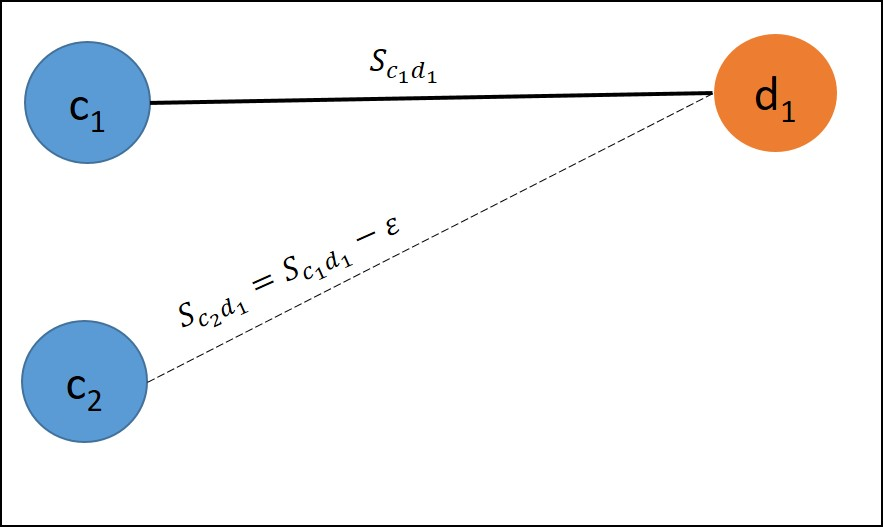
\includegraphics[width=\linewidth]{Graph/P1.jpg}
				\caption{Initial State}
				\label{fig:Initial State_}
			\end{subfigure}
			\begin{subfigure}{0.32\linewidth}
				\centering
				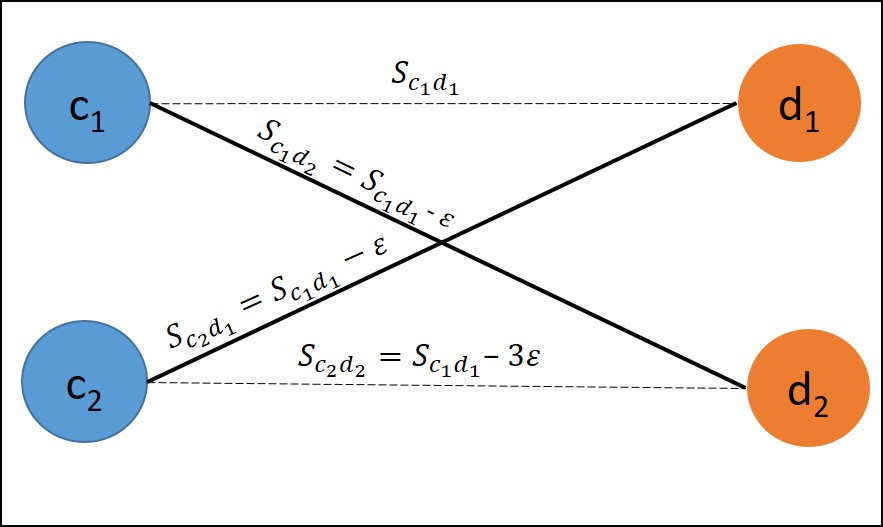
\includegraphics[width=\linewidth]{Graph/P3.jpg}
				\caption{Hungarian Algorithm}
				\label{fig:Hungarian}
			\end{subfigure}
			\begin{subfigure}{0.32\linewidth}
				%\vspace{.25cm}
				\centering
				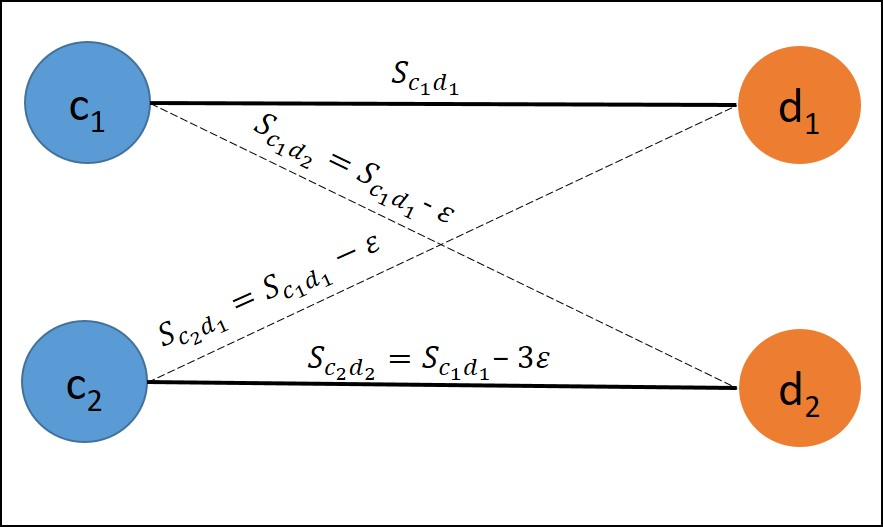
\includegraphics[width=\linewidth]{Graph/P2.jpg}
				\caption{ RORA and CRORA}
				\label{fig:Proposed Algorithm}
			\end{subfigure}
			
			
		}
	}%\vspace{-0.2cm}
	\caption{Assignment Strategy (Hungarian vs Proposed Algorithms)}
	\label{fig:Number of changes in assignment}
\end{figure*}


\begin{figure*}[t]
	{%
		\setlength{\fboxsep}{1.5pt}%
		\setlength{\fboxrule}{1.5pt}%
		\fbox{
			\begin{subfigure}{0.32\linewidth}
			    
				\centering
				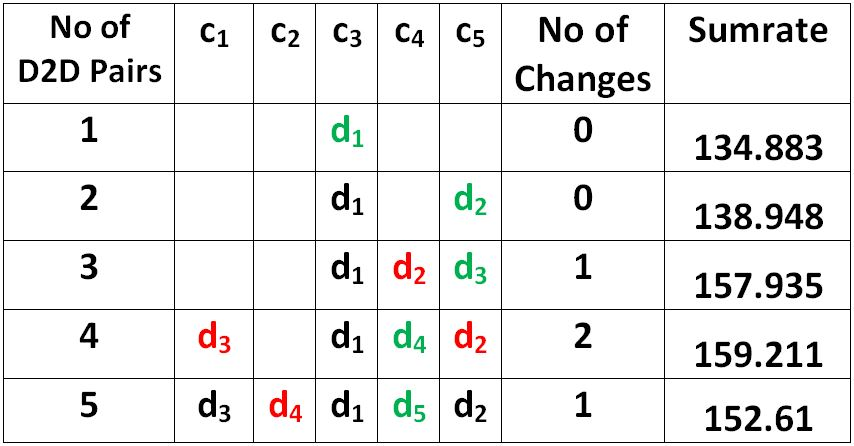
\includegraphics[width=\linewidth, height=35mm]{Graph/Hungarian.JPG}
				\caption{Hungarian Algorithm}
				\label{fig:trace_hungarian}
			\end{subfigure}
			\begin{subfigure}{0.32\linewidth}
				\centering
				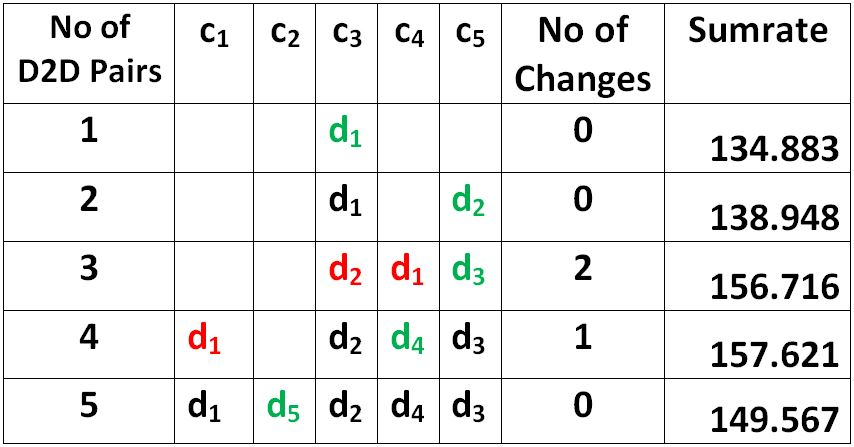
\includegraphics[width=\linewidth, height=35mm]{Graph/proposed1.JPG}
				\caption{RORA}
				\label{fig:trace_p1}
			\end{subfigure}
			\begin{subfigure}{0.32\linewidth}
				\centering
				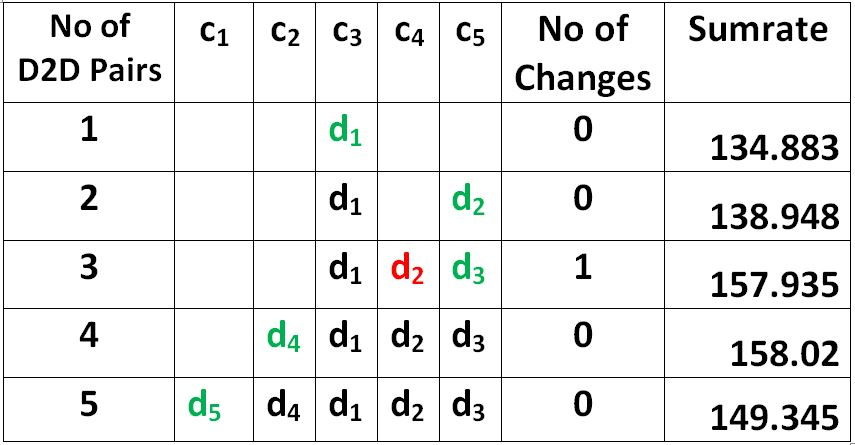
\includegraphics[width=\linewidth, height=35mm]{Graph/proposed2.JPG}
				\caption{CRORA}
				\label{fig:trace_p2}
			\end{subfigure}
			
			
		}
	}%
	\vspace{-0.2cm}
	\caption{Trace Analysis (Hungarian (Optimal) Algorithm vs Proposed Algorithms) }
	\label{fig:trace_analysis}
\end{figure*}


\section{Performance Evaluation}\label{section:Performation Evaluation}
\subsection{Different Algorithms for Performance Comparisons}
\noindent
We consider different resource allocation algorithms to compare the performance of our proposed algorithms (RORA and CRORA) in terms of total system sumrate and number of changes in assignment between two consecutive states of the system. Each of the algorithms is briefly explained here with their key points.

\subsubsection{Deferred Acceptance Based Algorithm for Resource Allocation (DARA)}
\noindent
DARA \cite{dara} also follows the stable matching algorithm presented in \cite{stable}. However, preferences for both the cellular UEs and the D2D pairs are calculated depending on their location. A device in close proximity is preferred over the far one. Depending on the given preference, a D2D pair selects a cellular UE to share the RBs. But distance is not the only factor behind better sumrate. It is assumed that a lower distance is preferred over a higher distance. However, a cellular UE experiences more interference from a nearby assigned D2D pair and we encounter such observations in our simulations. Moreover, in some cases this algorithm allows a cellular UE and a D2D pair to share the RBs even though QoS is not satisfied.

%\medskip
%\noindent A local search algorithm \cite{lora} is designed to solve the resource allocation problem where the target is to maximize the system sumrate while maintaining some QoS. The result of the greedy heuristic \cite{zulhasnine} is considered as the initial feasible solution of this algorithm. The final result of this greedy heuristic might miss out some assignments of D2D pairs which is considered in the optimal solution. These D2D pairs can also be missed out in the final assignments returned by this local search algorithm and in practice, the local optima of this algorithm can be far away from the global solution. Moreover, as local search is an iterative improvement technique, it might take much more time to reach the solution and can not be very useful in LTE and beyond networks.

\subsubsection{Local Search Based Resource Allocation Algorithm (LORA)} 
\noindent
A local search algorithm LORA \cite {lora} uses the allocation given by the greedy algorithm \cite{zulhasnine} as the initial feasible solution. Then it swaps assignment between a D2D pair and a cellular UE only if the swapping improves the objective function, as well as the constraints,  are satisfied. LORA can also face the similar problem encountered by the greedy algorithm \cite{zulhasnine}. The final result of the greedy heuristic might miss out some of the D2D pairs for assignments those are considered in the optimal solution. These D2D pairs can also be missed out in the final assignments returned by the local search algorithm and in practice, the local optima of this algorithm can be far away from the global solution.
% Moreover, as local search is an iterative improvement technique, it might take much more time to reach the solution and can not be very useful in LTE and beyond networks.
%So, that particular D2D pair can be unassigned at the end of the local search algorithm. It is very easy to find an example, where such a D2D pair can be assigned in the optimal solution.


\subsubsection{Optimal Algorithm}

\noindent
Hungarian algorithm \cite{hungarian} is a weighted bipartite matching based algorithm used in \cite {zhang},\cite{feng},\cite{ccnc} for similar resource allocation problems in D2D communications. Hungarian algorithm is an optimal algorithm that outperforms other heuristics. In our simulation study, we also consider a similar algorithm \cite{hungarian}.

\smallskip
\par
\noindent
In simulation graphs, our proposed algorithms are named as "RORA" and "CRORA" and the optimal Hungarian algorithm is named as "optimal".


\subsection{Simulation Environment}

\noindent
We simulate different scenarios to evaluate the efficiency of our proposed algorithms (RORA and CRORA). We use the C++ programming language to build our simulator that supports LTE system. The research problem we consider is a type of assignment problem which is one of the fundamental combinatorial optimization problems in the branch of optimization. In our simulation, our main objective is to find the assignments of the D2D pairs with the cellular UEs. Based on the assignments, we need to calculate SINR, interference and system sumrate from their respective equations. We need to mention that as we do not need to implement the PHY, MAC and network layer to implement our proposed relax online resource allocation algorithms so a networking simulator is not essential for our simulation study. 
\noindent
We use the same simulation parameters (Table~\ref{Simulation_table}) as in \cite{lora},\cite{zulhasnine},\cite{dara} as well as some other variants of these parameters for the performance evaluation of the proposed algorithms. A single cell network is considered in the simulations. We consider that the cellular UEs and the D2D pairs are uniformly distributed in the cell area where D2D pairs (D2D transmitters and D2D receivers) are uniformly distributed in a random cluster with a maximum radius of $15$ meters. All of the simulation results presented in this paper are an average of $50$ different runs for a particular scenario.  



\begin{table}[]
%to pad the row
\renewcommand{\arraystretch}{1.2}
%\centering
\vspace{-0.2cm}
\caption{Simulation Parameters}
\label{Simulation_table}
\vspace{-0.2cm}
\centerline{
\begin{tabular}{|c|c|}
\hline
\textbf{Parameter}           & \textbf{Value}               \\ \hline 
Cell Radius                  & $1000$ meters                  \\ \hline
Maximum D2D pair distance    & $15$ meters                    \\ \hline
Cellular user transmit power & $20$ dBm                       \\ \hline
D2D transmit power           & $20$ dBm                       \\ \hline
Base Station transmit power  & $46$ dBm                       \\ \hline
Noise power (AWGN)           & $-174$ dBm                     \\ \hline
Carrier Frequency            & $1.7$ GHz for LTE              \\ \hline
$\gamma_{c_i,target}^{DL}$     & Random                        \\ \hline
$\gamma_{d_j,target}^{DL} $    & Random                 \\ \hline
\end{tabular}}
\vspace{-0.4cm}
\end{table}




%\begin{figure*}[t]
%	{%
%		\setlength{\fboxsep}{1.5pt}%
%		\setlength{\fboxrule}{1.5pt}%
%		\fbox{
%			\begin{subfigure}{0.32\linewidth}
%				\centering
%				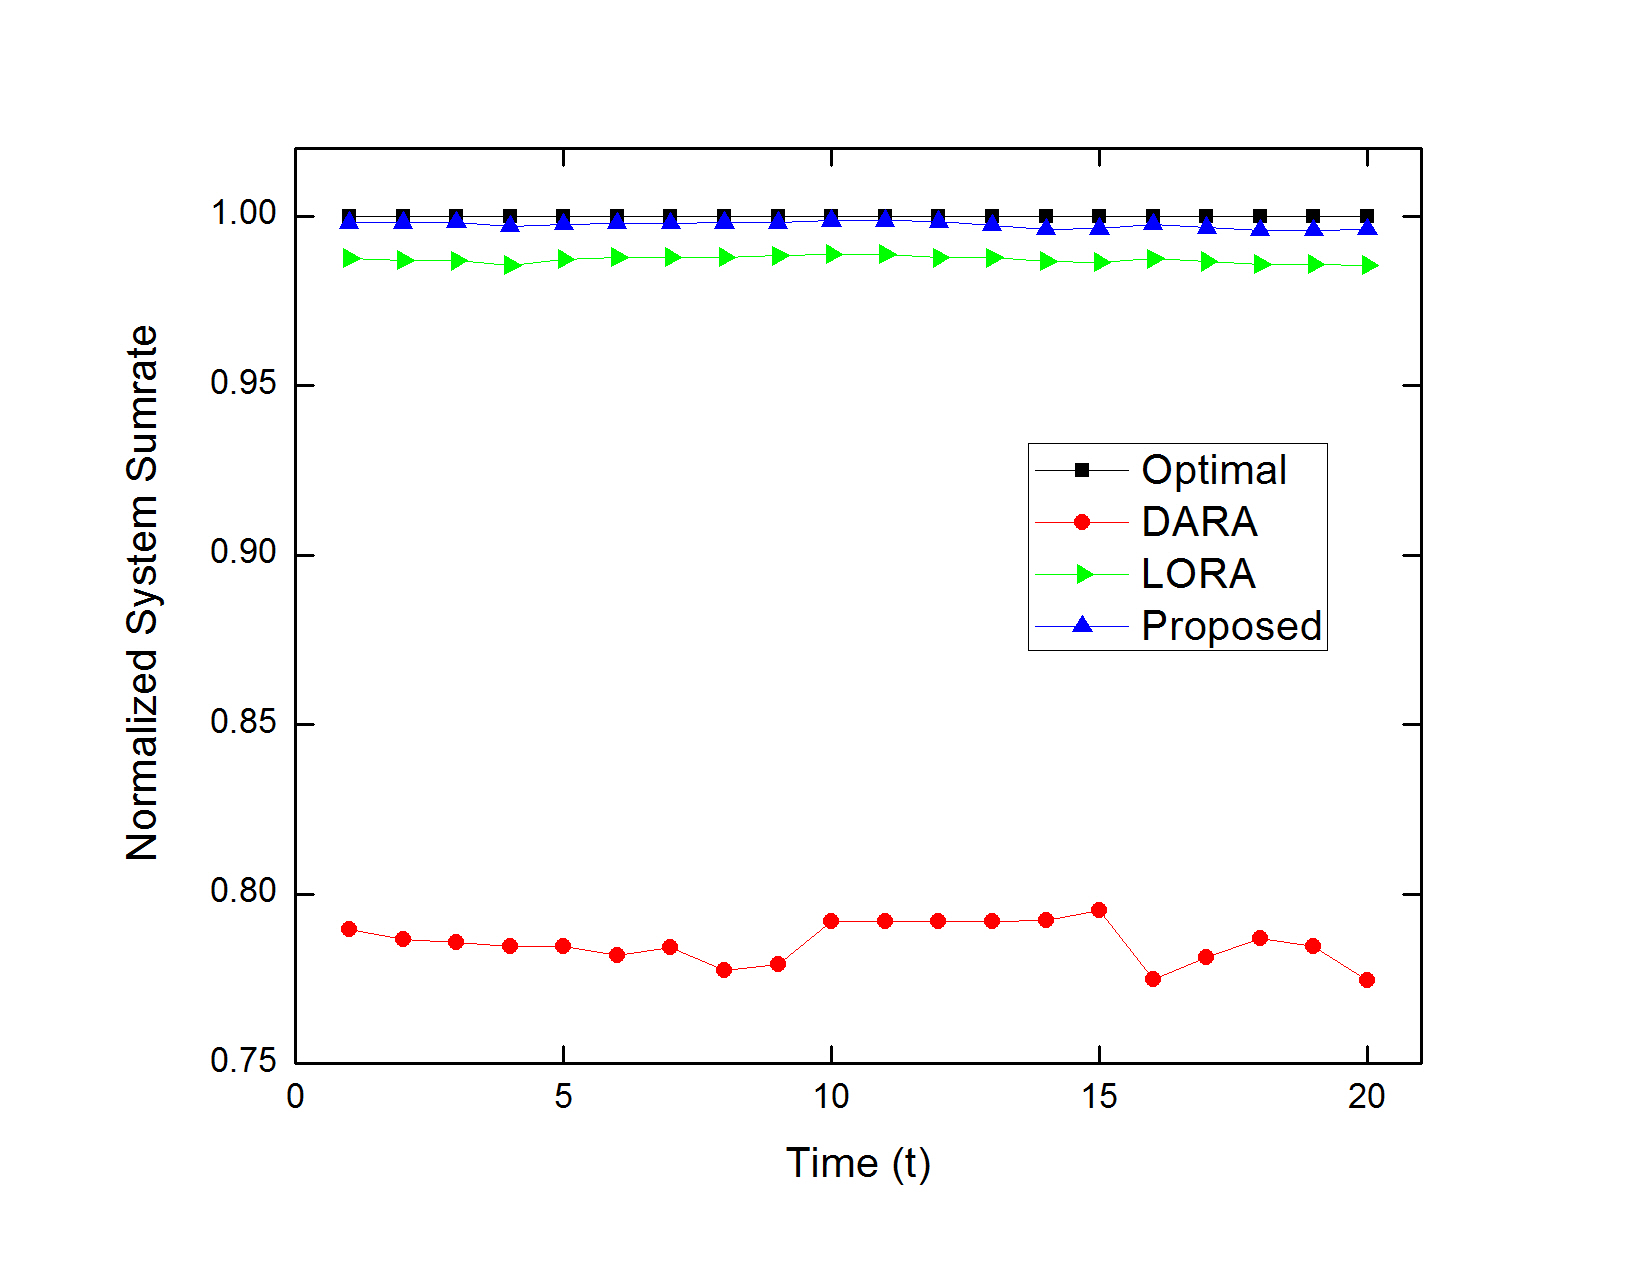
\includegraphics[width=\linewidth]{Graph/sumrate_f.jpg}
%				\caption{Normalized system sumrate of RA algorithms in each states  (Normalized with respect to the optimal algorithm)}
%				\label{fig:sumrate_f}
%			\end{subfigure}
%			\begin{subfigure}{0.32\linewidth}
%				\centering
%				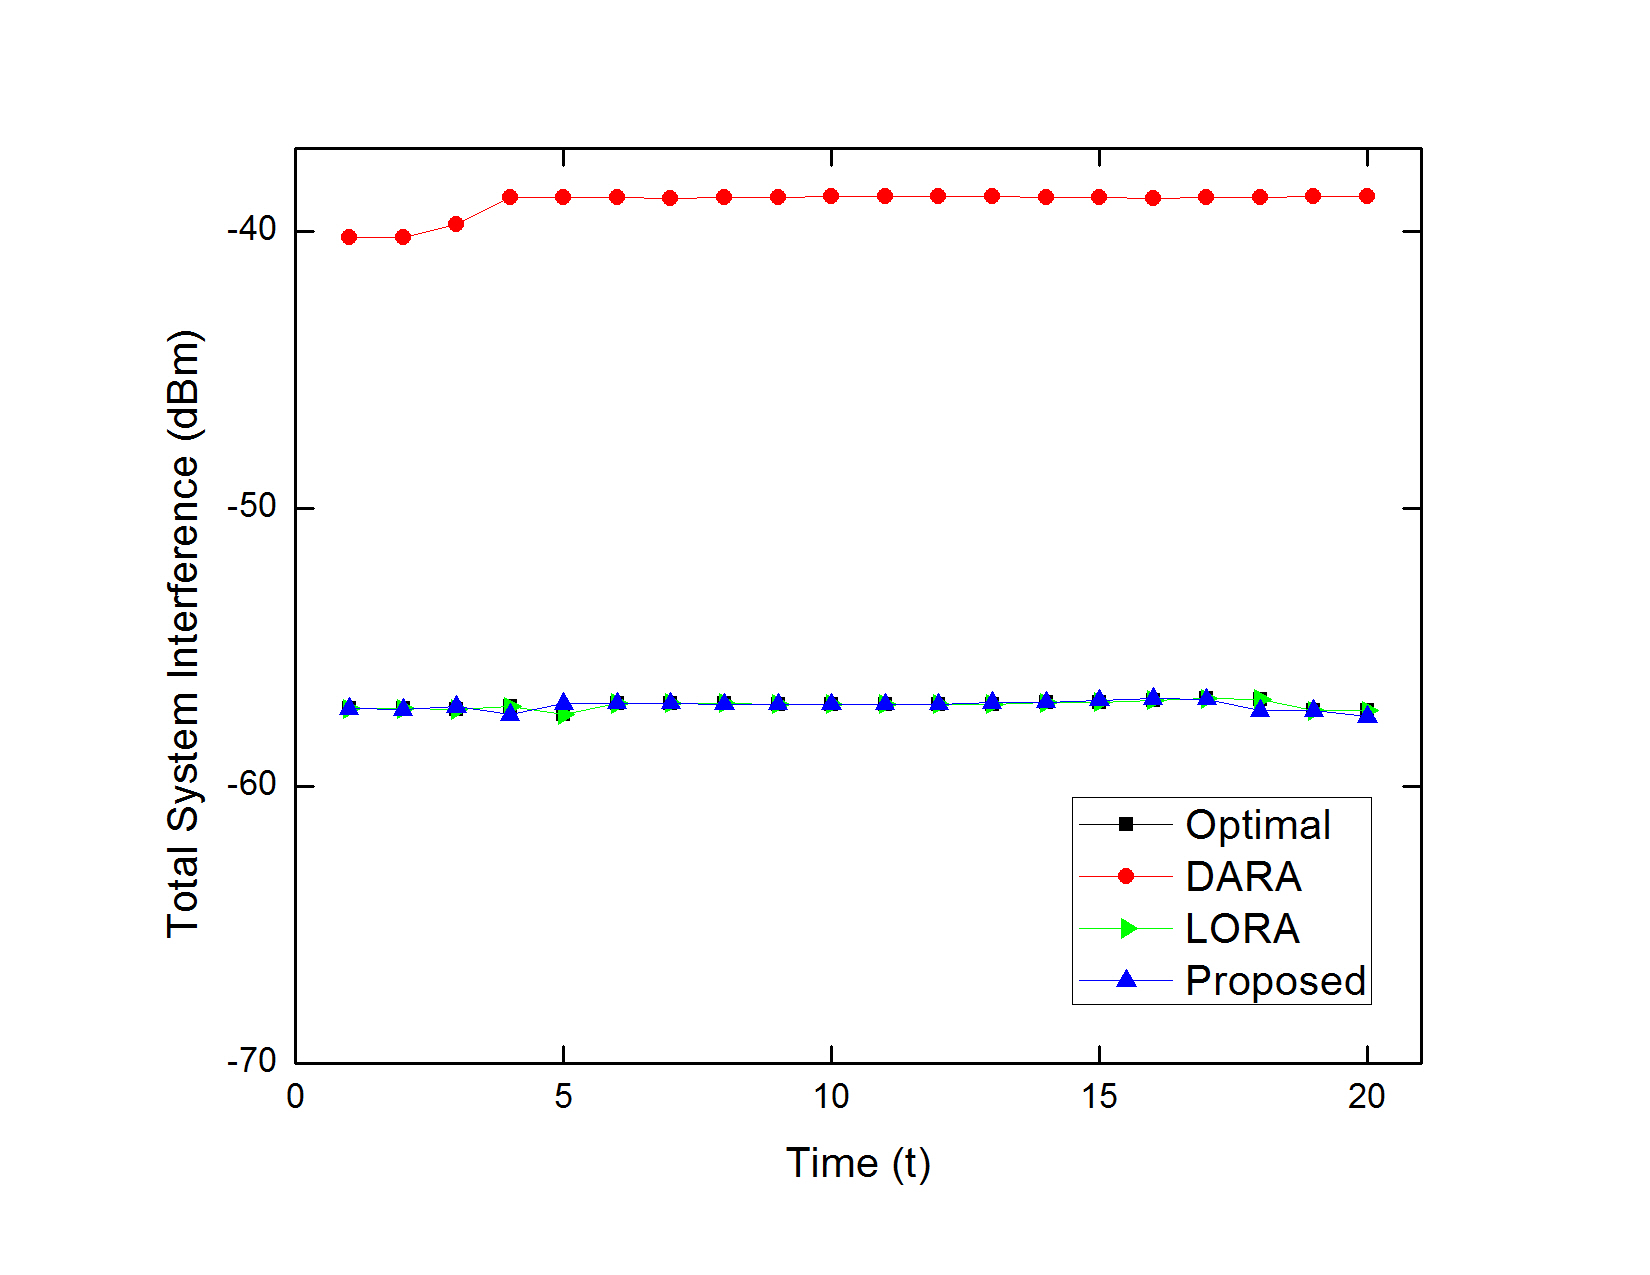
\includegraphics[width=\linewidth]{Graph/inter_f.jpg}
%				\caption{Total system interference of RA algorithms in each states}
%				\label{fig:inter_f}
%			\end{subfigure}
%			\begin{subfigure}{0.32\linewidth}
%				\centering
%				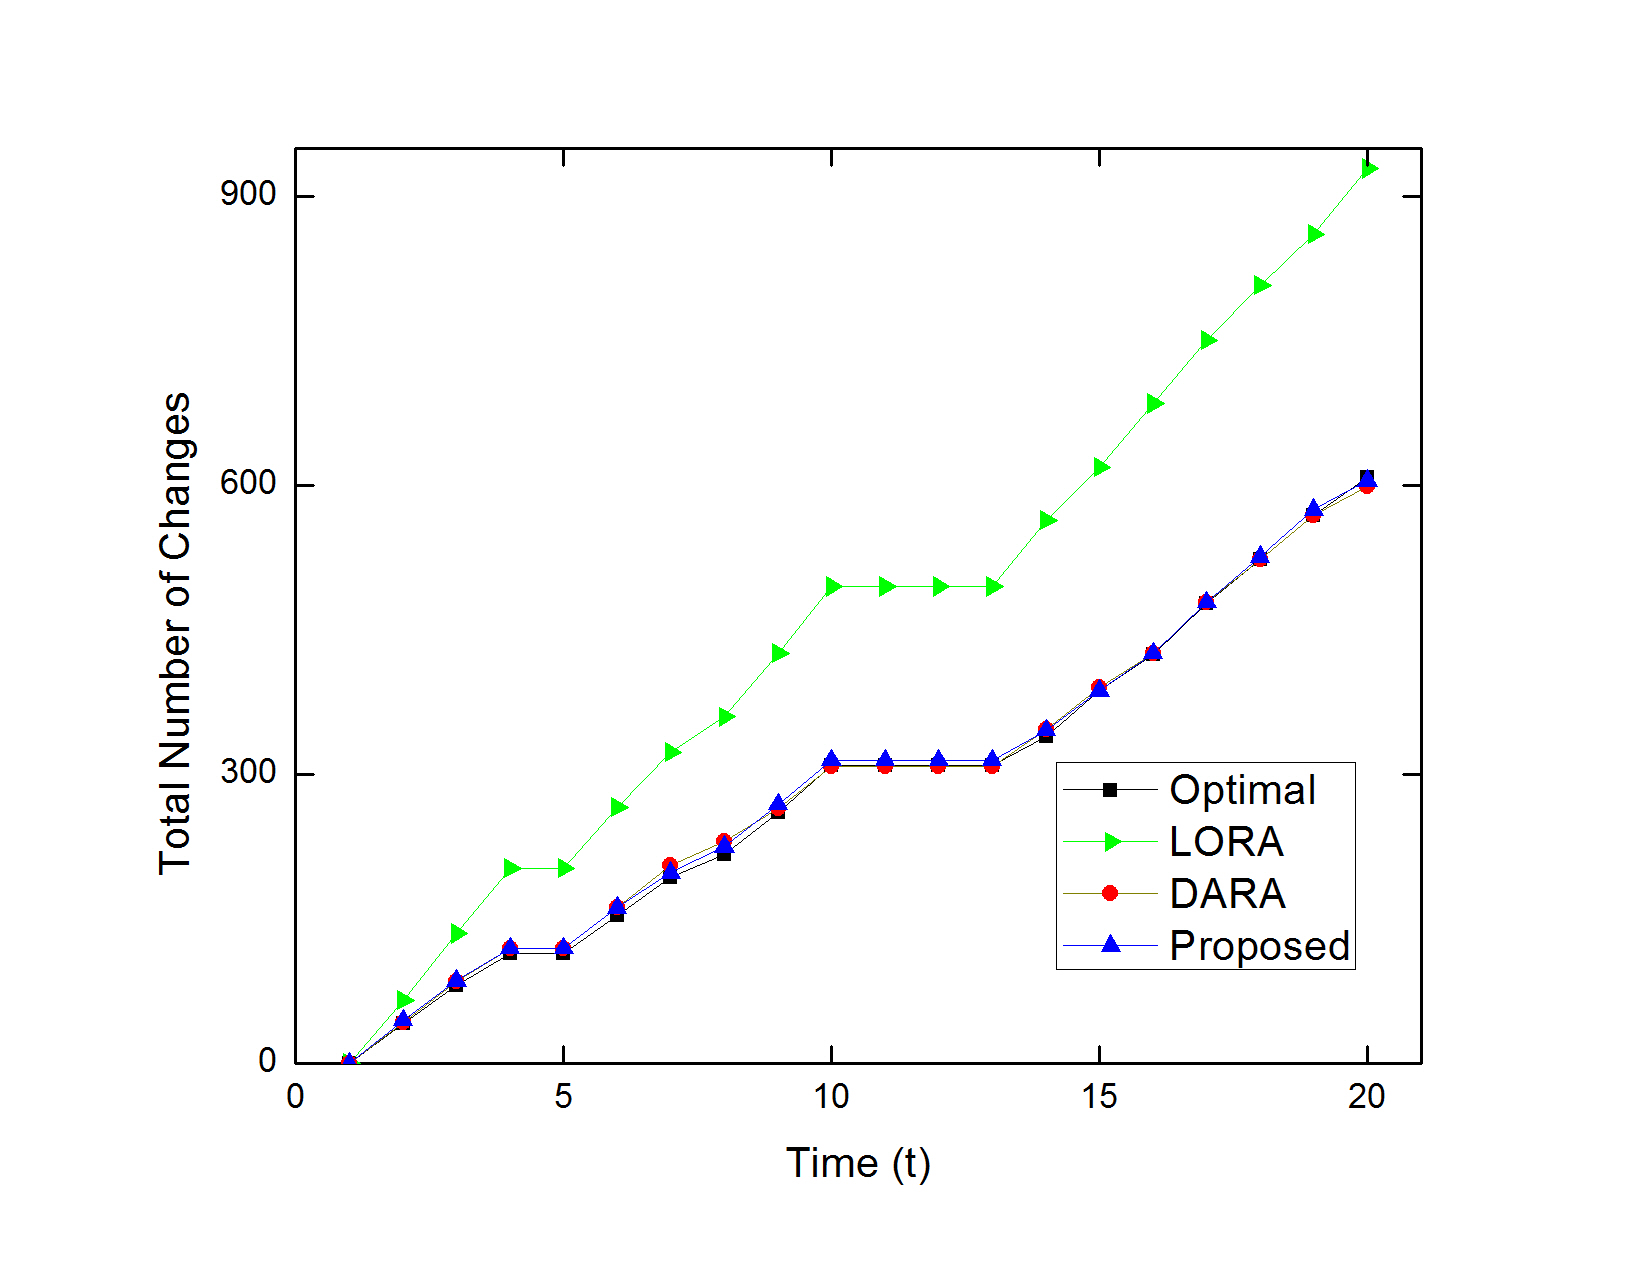
\includegraphics[width=\linewidth]{Graph/noc_f.jpg}
%				\caption{Total Number of changes in Cellular UEs}
%				\label{fig:noc_f}
%			\end{subfigure}
%			
%			
%		}
%	}%
%	\caption{Performance evaluation of fair assignment}
%	\label{fig:fair_perform}
%\end{figure*}
%
%\begin{figure*}[t]
%	{%
%		\setlength{\fboxsep}{1.5pt}%
%		\setlength{\fboxrule}{1.5pt}%
%		\fbox{
%			\begin{subfigure}{0.32\linewidth}
%				\centering
%				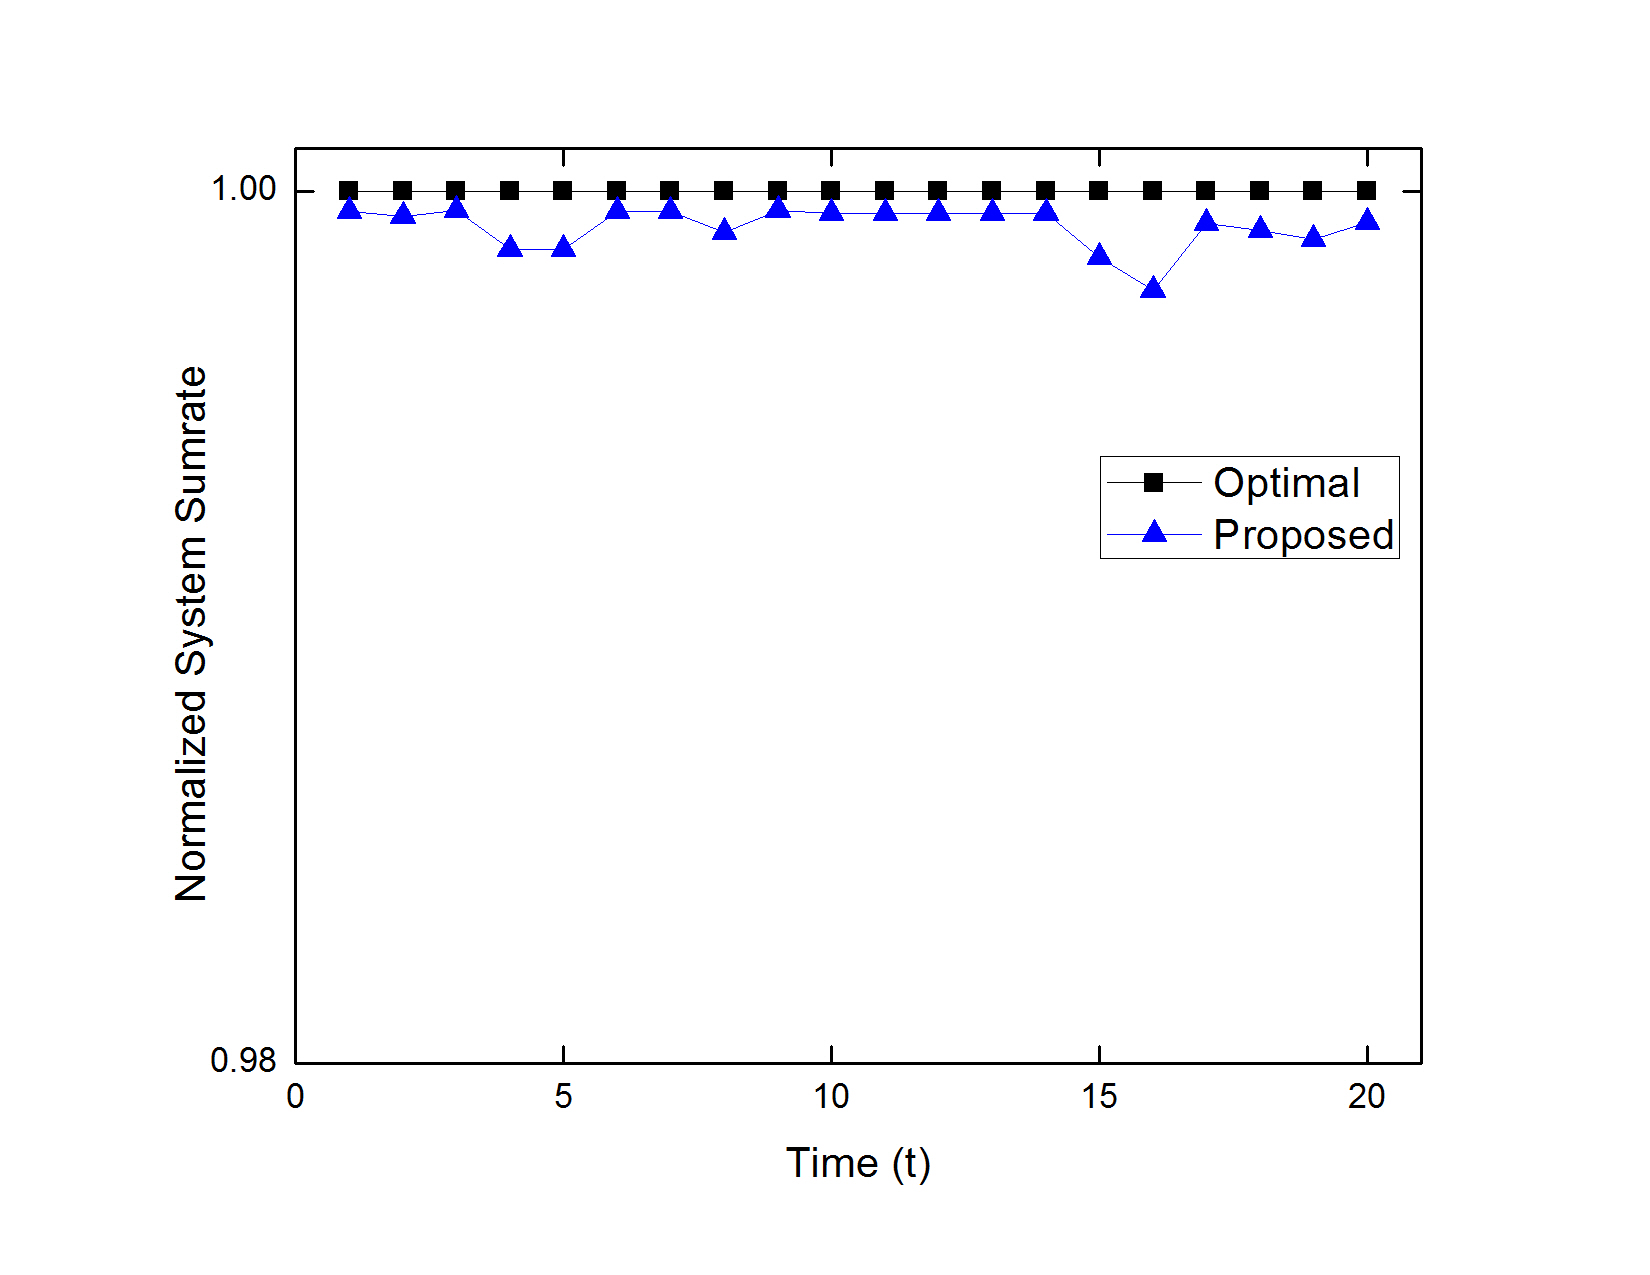
\includegraphics[width=\linewidth]{Graph/sumrate_unfair.jpg}
%				\caption{Normalized system sumrate of RA algorithms in each states  (Normalized with respect to the optimal algorithm)}
%				\label{fig:sumrate_unfair}
%			\end{subfigure}
%			\begin{subfigure}{0.32\linewidth}
%				\centering
%				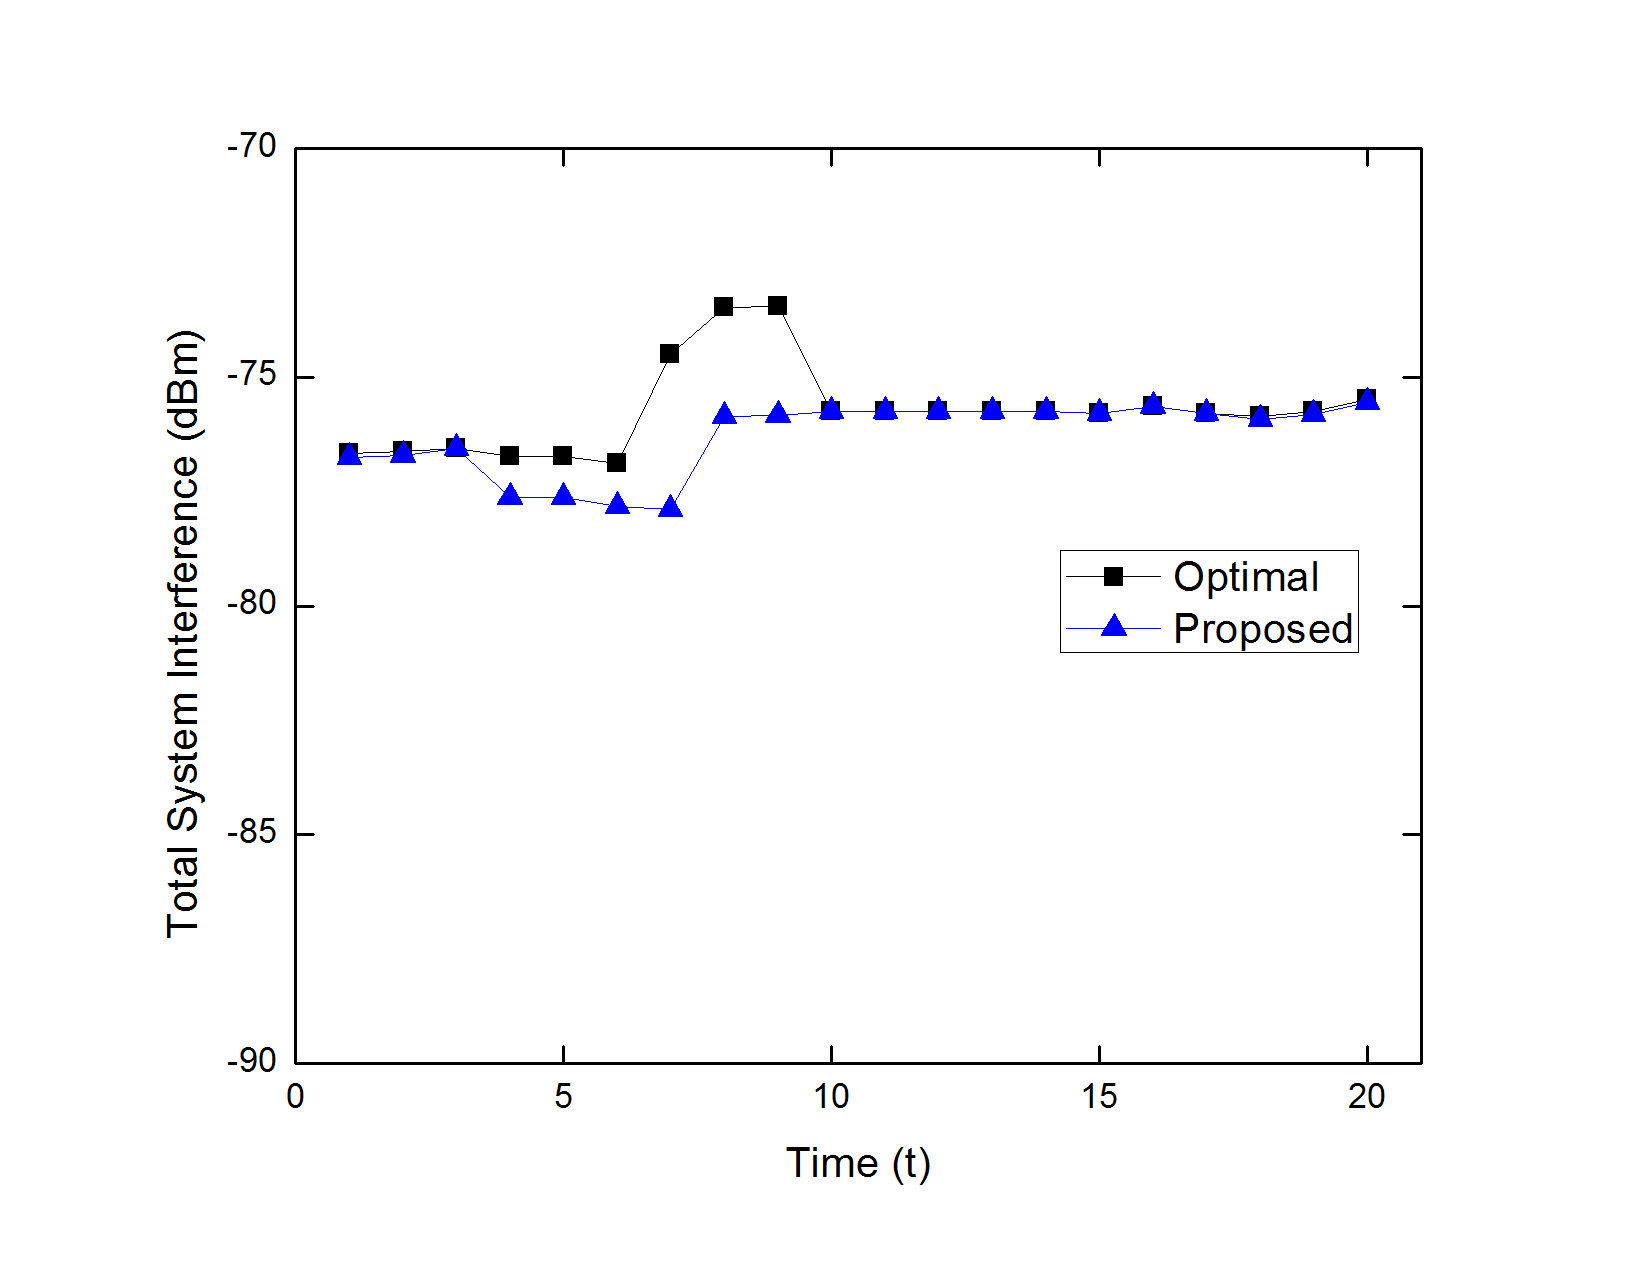
\includegraphics[width=\linewidth]{Graph/inter_unfair.jpg}
%				\caption{Total system interference of RA algorithms in each states}
%				\label{fig:inter_unfair}
%			\end{subfigure}
%			\begin{subfigure}{0.32\linewidth}
%				\centering
%				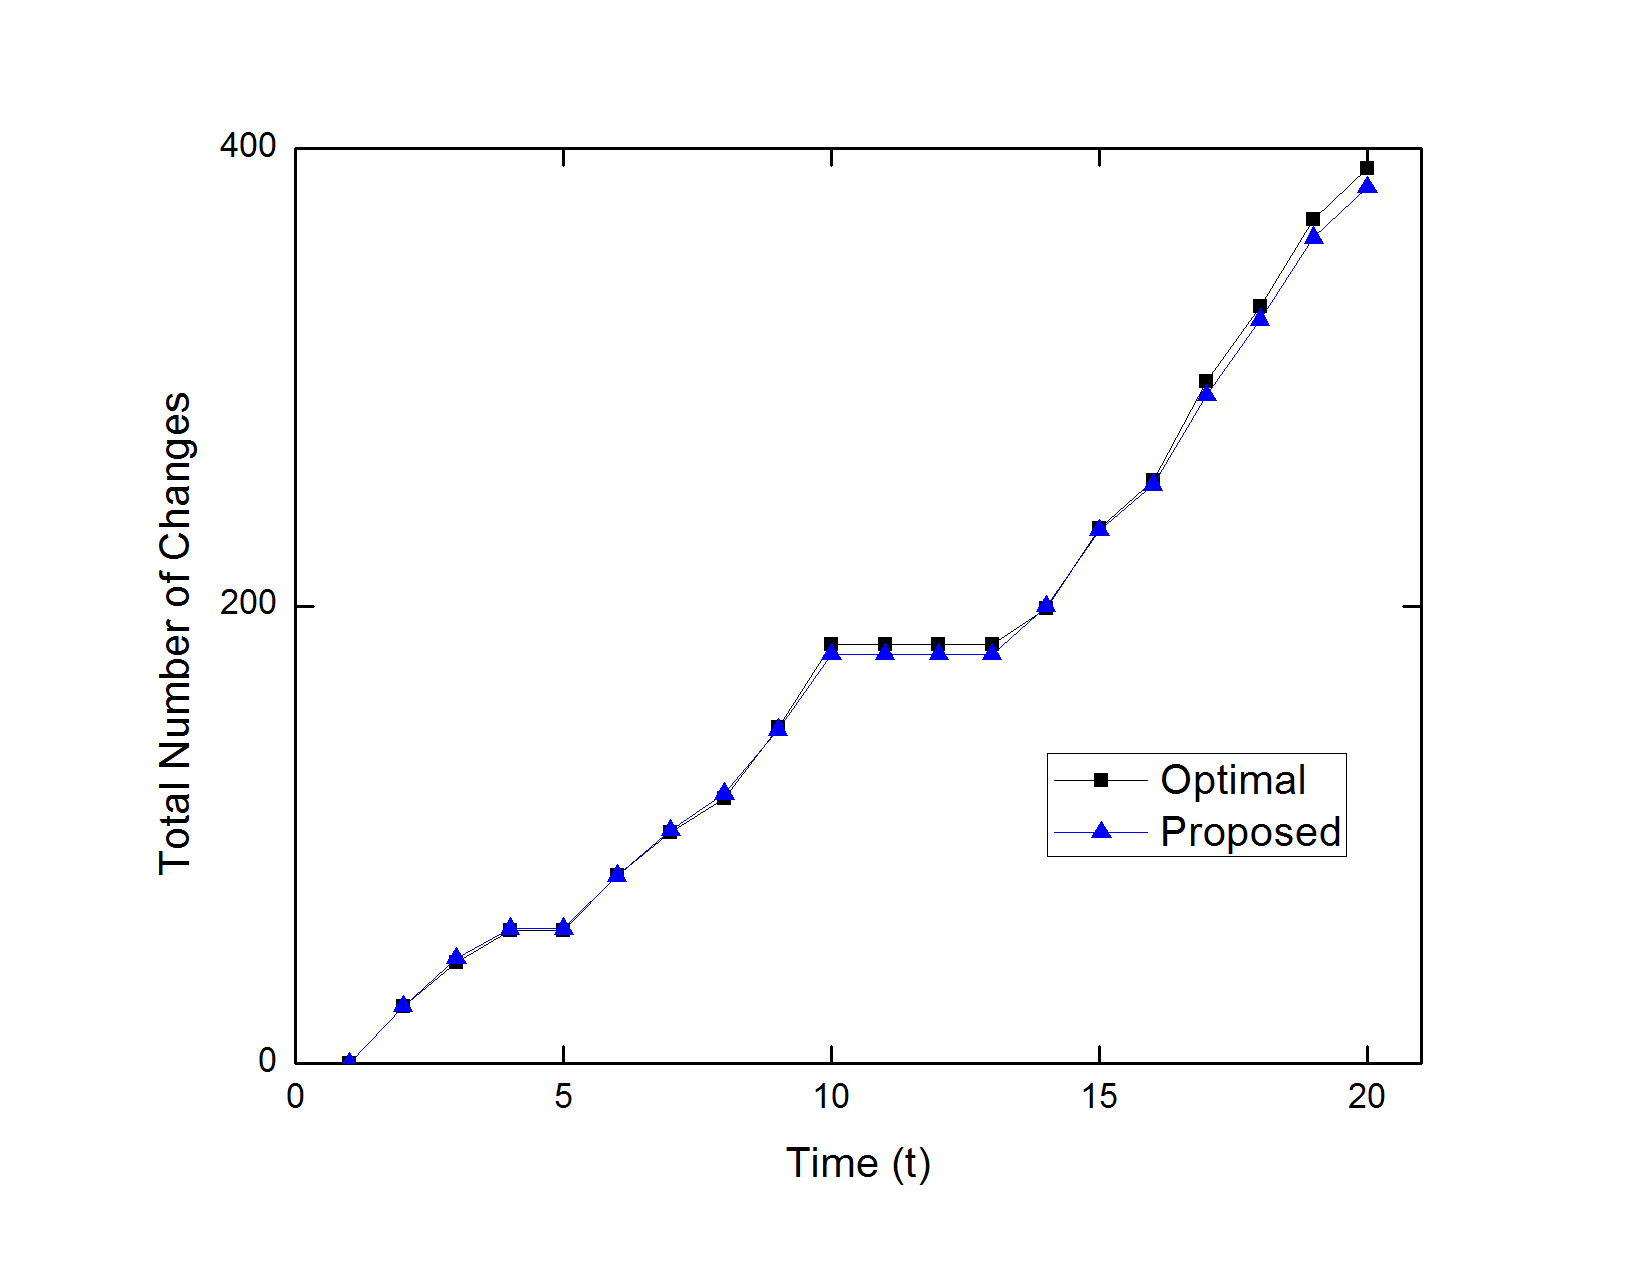
\includegraphics[width=\linewidth]{Graph/noc_uf.jpg}
%				\caption{Total Number of changes in Cellular UEs}
%				\label{fig:noc_uf}
%			\end{subfigure}
%			
%			
%		}
%	}%
%	\caption{Performance evaluation of restricted assignment}
%	\label{fig:restrict_perform}
%\end{figure*}



\subsection{Input Data Model}

\noindent

% We need to change this subsection wiht the MMPP and poissoin process 

\noindent
For all of the simulation results presented in this paper, we start with $300$ cellular UEs and a single D2D pair. Based on the system events the number of D2D pairs in the system varies over time whereas the number of cellular UEs is fixed. We stop the simulation when the number of D2D pairs in the system becomes $225$ ( $75\%$ of the number of the cellular UEs as we are considering a system where the number of the cellular UEs is much greater than the number of the D2D pairs). However, based on the mobility system event the relative positions of both the D2D pairs and the cellular UEs change over time. We use Markov Modulated Poisson Process (MMPP)\cite{salvador2003multiscale} to model the arrival and mobility event. With MMPP arrival/mobility event rate $\lambda_s$ is determined by the phase $s$ of the Markov chain \cite{stewart1994introduction}, where the total number of states is S (i.e., s = 1,2,. . . ,S). In our simulation, we consider only two states of the Markov chain working in a discrete time where $\lambda_1$ is the rate of state $1$ and $\lambda_2$ is the rate of state $2$. So, we can say both arrival event (D2D pairs) and mobility event (both D2D pairs and cellular UEs) are modeled using discrete time Markov Modulated Poisson Process (dMMPP). At the time of an arrival event, we consider any random number of D2D pairs in between $1$ and $9$. However, our algorithm can handle any number of D2D pairs at a single arrival event. Moreover, we perform extensive simulations with a different number of cellular users and a different number of initial D2D pairs with different arrival rates and we find that all of the simulation results are almost identical to the result we present here in terms of performance.

% Here we need to put the information the the total time and final number of D2D 
%In every single run of our simulation we consider $40$ discrete events of D2D arrival and 
%After all the $40$ events the final number of D2D pairs present in the system is $208$.
\noindent


\subsection{Result Comparison}

%Figure \ref{fig:fair_perform} and \ref{fig:restrict_perform} compares our proposed algorithm based on the preference list.
%In \ref{fig:fair_perform} our proposed algorithm is compared with optimal, DARA and LORA. On the other hand, \ref{fig:restrict_perform} proposed algorithm is only compared with optimal one as there is no existing variant of restricted version. In \ref{fig:sumrate_f}, \ref{fig:sumrate_unfair}  sumrate is compared. Our proposed algorithm situated just after the optimal algorithm. In the case of interference, it is observed from figure \ref{fig:inter_f} and \ref{fig:inter_unfair} that optimal, LORA and proposed algorithm is very close to each other. In case of the number of changes in Cellular UE figure \ref{fig:noc_f} and \ref{fig:noc_uf} show that our proposed algorithm changes a minimum number of assignment. From this observation, we can readily say that our proposed algorithm offers a good online algorithm.




%\smallskip
\noindent
We compare our proposed algorithms (RORA and CRORA) with the existing offline algorithms for both of the fair assignment scheme and the restricted assignment scheme. For both of the assignment schemes, we compare the algorithms with respect to the total system sumrate and number of changes in assignment between two successive allocations. Figure \ref{fig:sum_f} represents the comparison of the total system sumrate returned by the algorithms in different states of the system for the fair assignment scheme. From the graph presented in Figure \ref{fig:sum_f}, we can observe that both RORA and CRORA perform very close to the optimal algorithm and LORA performs next to our proposed algorithms whereas DARA performs the worst. The reason for DARA's poor performance is that the preference list of DARA is based on the increasing order of the proximity which is not the best approach for this optimization problem. For clarity we present the normalized system sumrates returned by different algorithms in Figure \ref{fig:sum_f_N} where the graph is normalized with respect to the optimal algorithm. From Figure \ref{fig:sum_f_N} we can observe that in the fair allocation scheme both RORA and CRORA performs almost $99.95\%$ of the optimal algorithm and by a very narrow margin CRORA outperforms RORA  in terms of total system sumrate. Figure  \ref{fig:noc_f} represents the comparison of different algorithms in term of the number of changes in successive allocation. We exclude DARA from this comparison as it performs remarkably poor in term of system sumrate. Figure \ref{fig:noc_f} suggests that both RORA and CRORA outperform LORA and the optimal algorithm where the individual line represents cumulative number of changes for different algorithms in discrete time event. RORA performs approximately $55\%$ less number of changes than LORA and $5\%$ less number of changes than the optimal algorithm whereas CRORA performs remarkably approximately $92\%$ less number of changes than LORA and $75\%$ less number of changes than the optimal algorithm. In term of the number of changes CRORA outperforms RORA by performing approximately $70\%$ less number of changes in assignment between two successive states. 

\begin{figure}[t]
	{ %
		\setlength{\fboxsep}{1.5pt}%
		\setlength{\fboxrule}{1.5pt}%
		\centering
		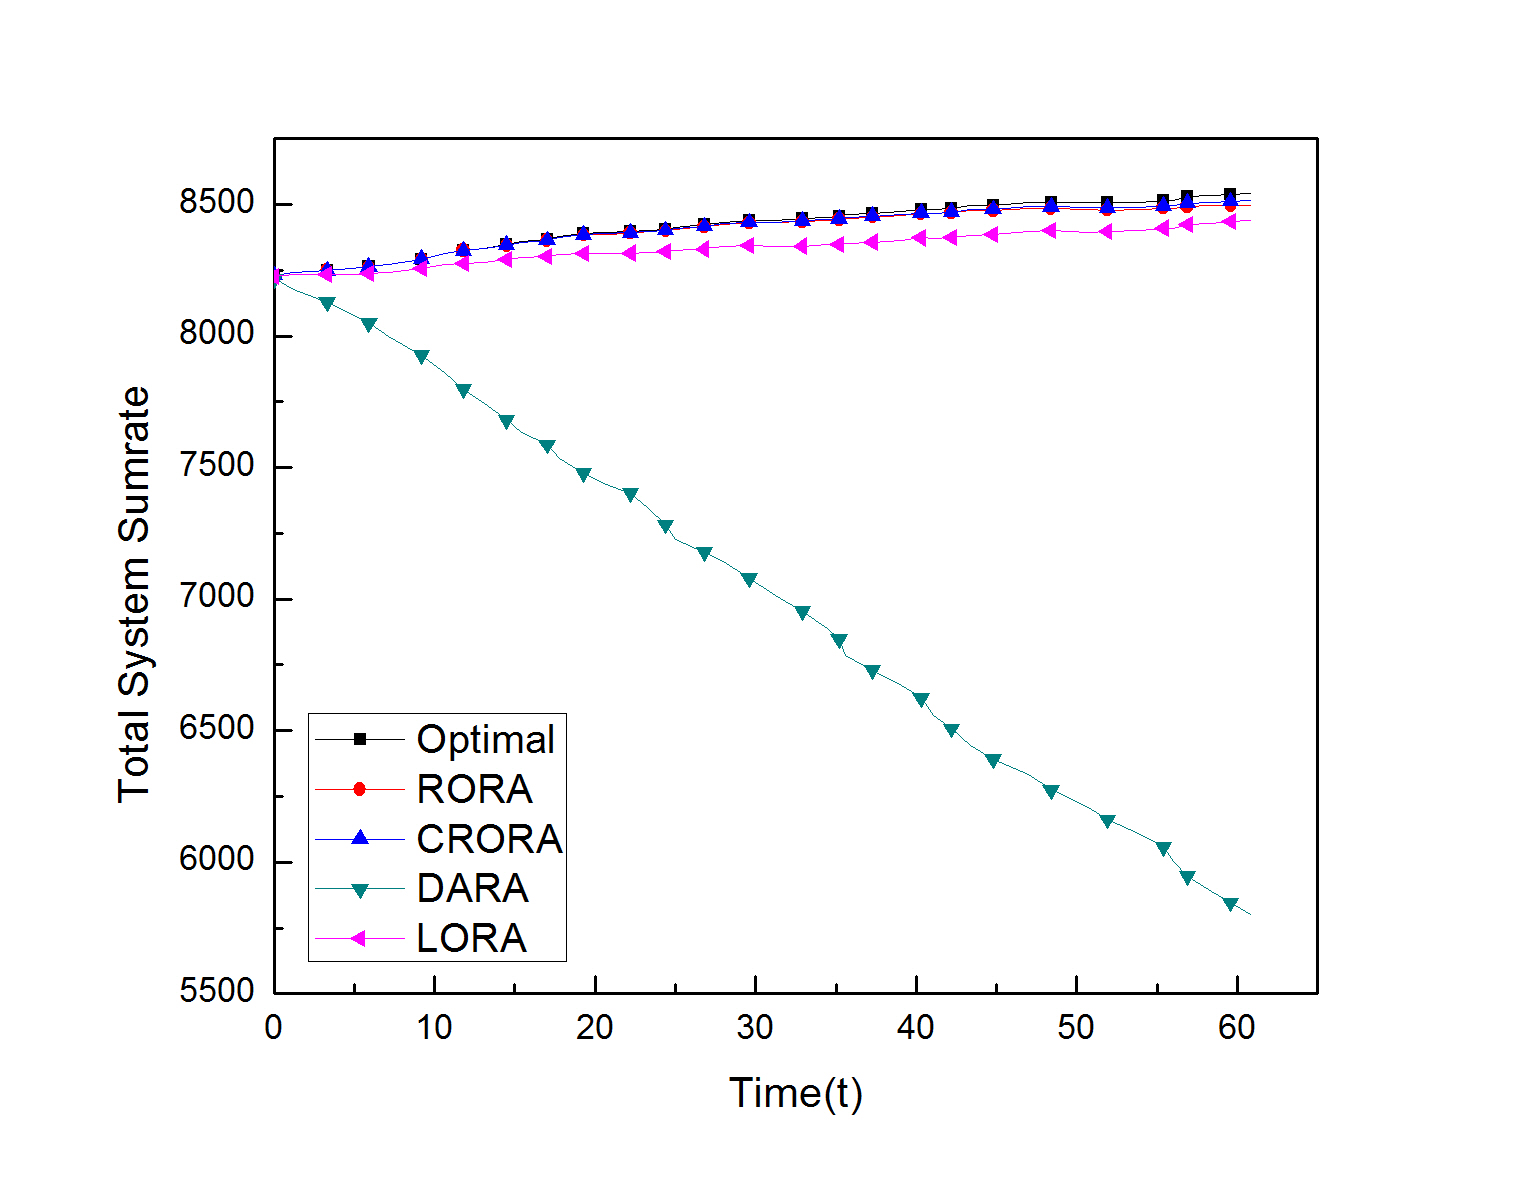
\includegraphics[width=90mm,height=60mm]{Graph/sumrateFairJournal.jpg}
		\vspace{-0.2cm}
		\caption{Total System Sumrate in Each State of the System for the Fair Assignment Scheme }
		 \label{fig:sum_f}
	}
	\vspace{-.5cm}
\end{figure}

\begin{figure}[t]
	{ %
		\setlength{\fboxsep}{1.5pt}%
		\setlength{\fboxrule}{1.5pt}%
		\centering
		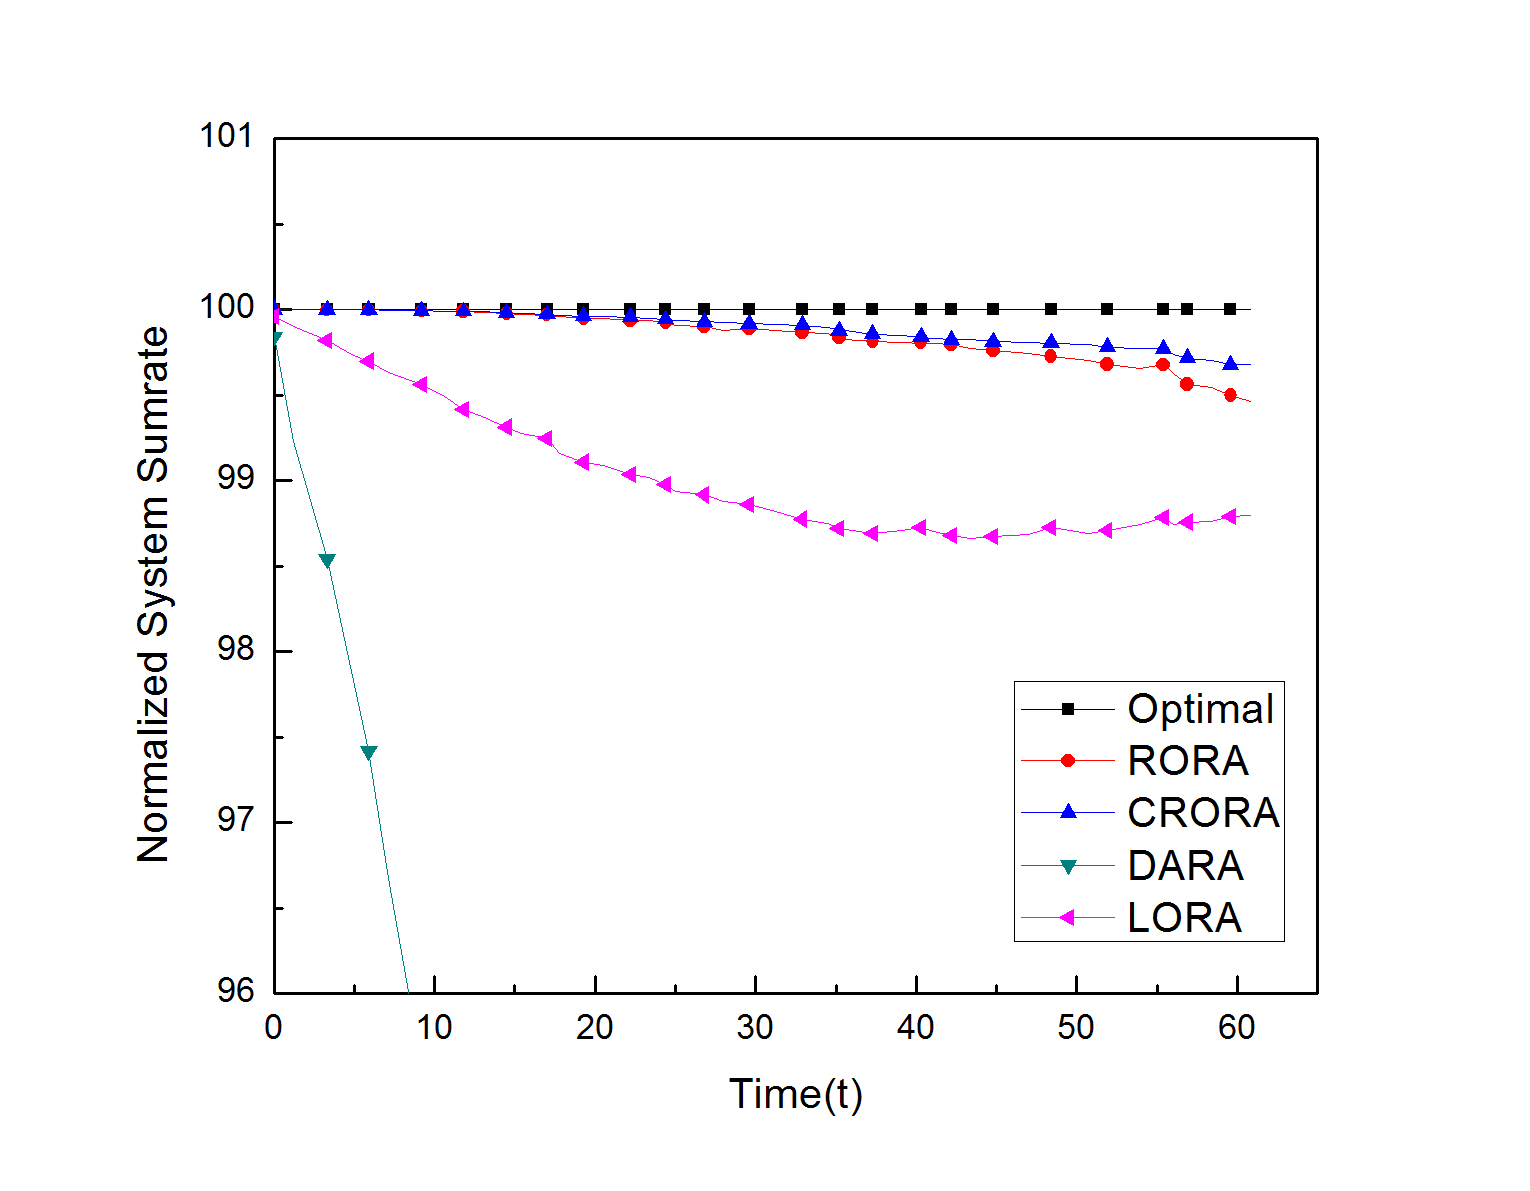
\includegraphics[width=90mm,height=60mm]{Graph/NormalizedsumrateFairJournal.jpg}
		\vspace{-0.2cm}
		\caption{Normalized System Sumrate in Each State of the System for the Fair Assignment Scheme (Normalized with Respect to the Optimal Hungarian Algorithm)} \label{fig:sum_f_N}
	}
	\vspace{-.5cm}
\end{figure}

\begin{figure}[t]
	{ %
	    %\vspace{-.5cm}
		\setlength{\fboxsep}{1.5pt}%
		\setlength{\fboxrule}{1.5pt}%
		\centering
		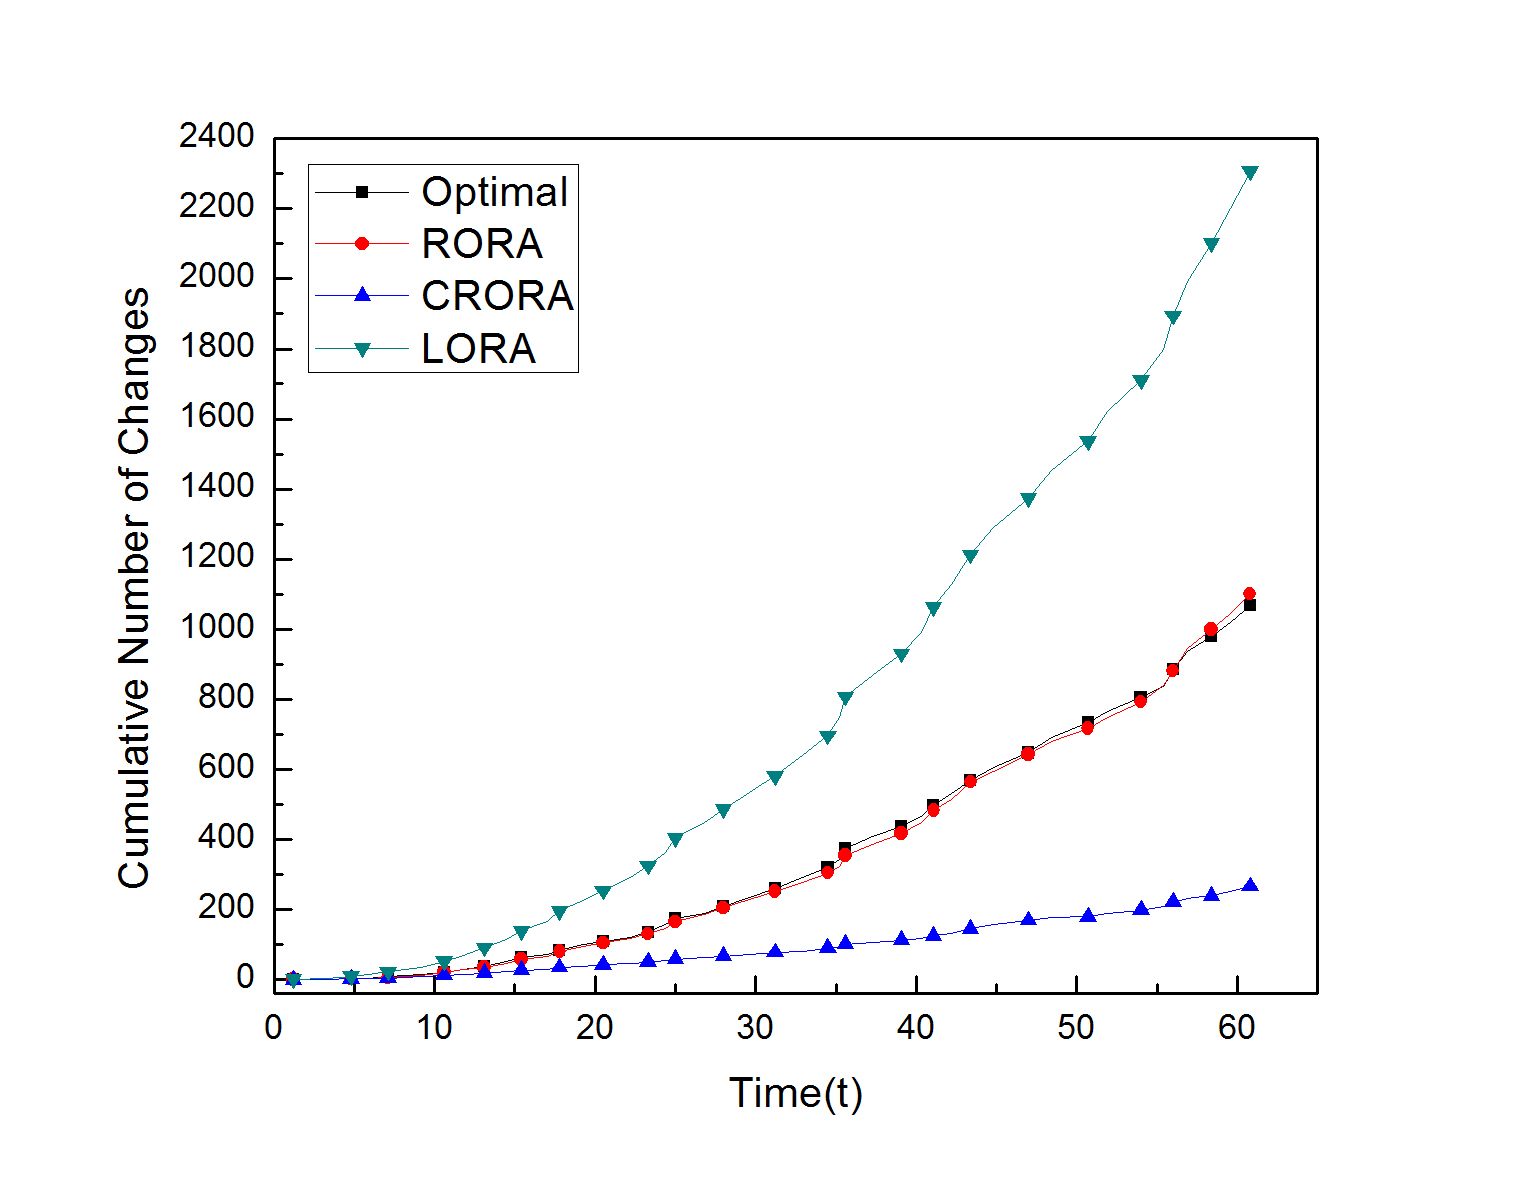
\includegraphics[width=90mm,height=60mm]{Graph/nocFairjournal.jpg}
		\vspace{-0.2cm}
		\caption{Cumulative Number of Changes in Each State of the System for the Fair Assignment Scheme}
		\vspace{-.5cm}
		\label{fig:noc_f}
		
	}
\end{figure}


\begin{figure}[t]
	{ %
		\setlength{\fboxsep}{1.5pt}%
		\setlength{\fboxrule}{1.5pt}%
		\centering
		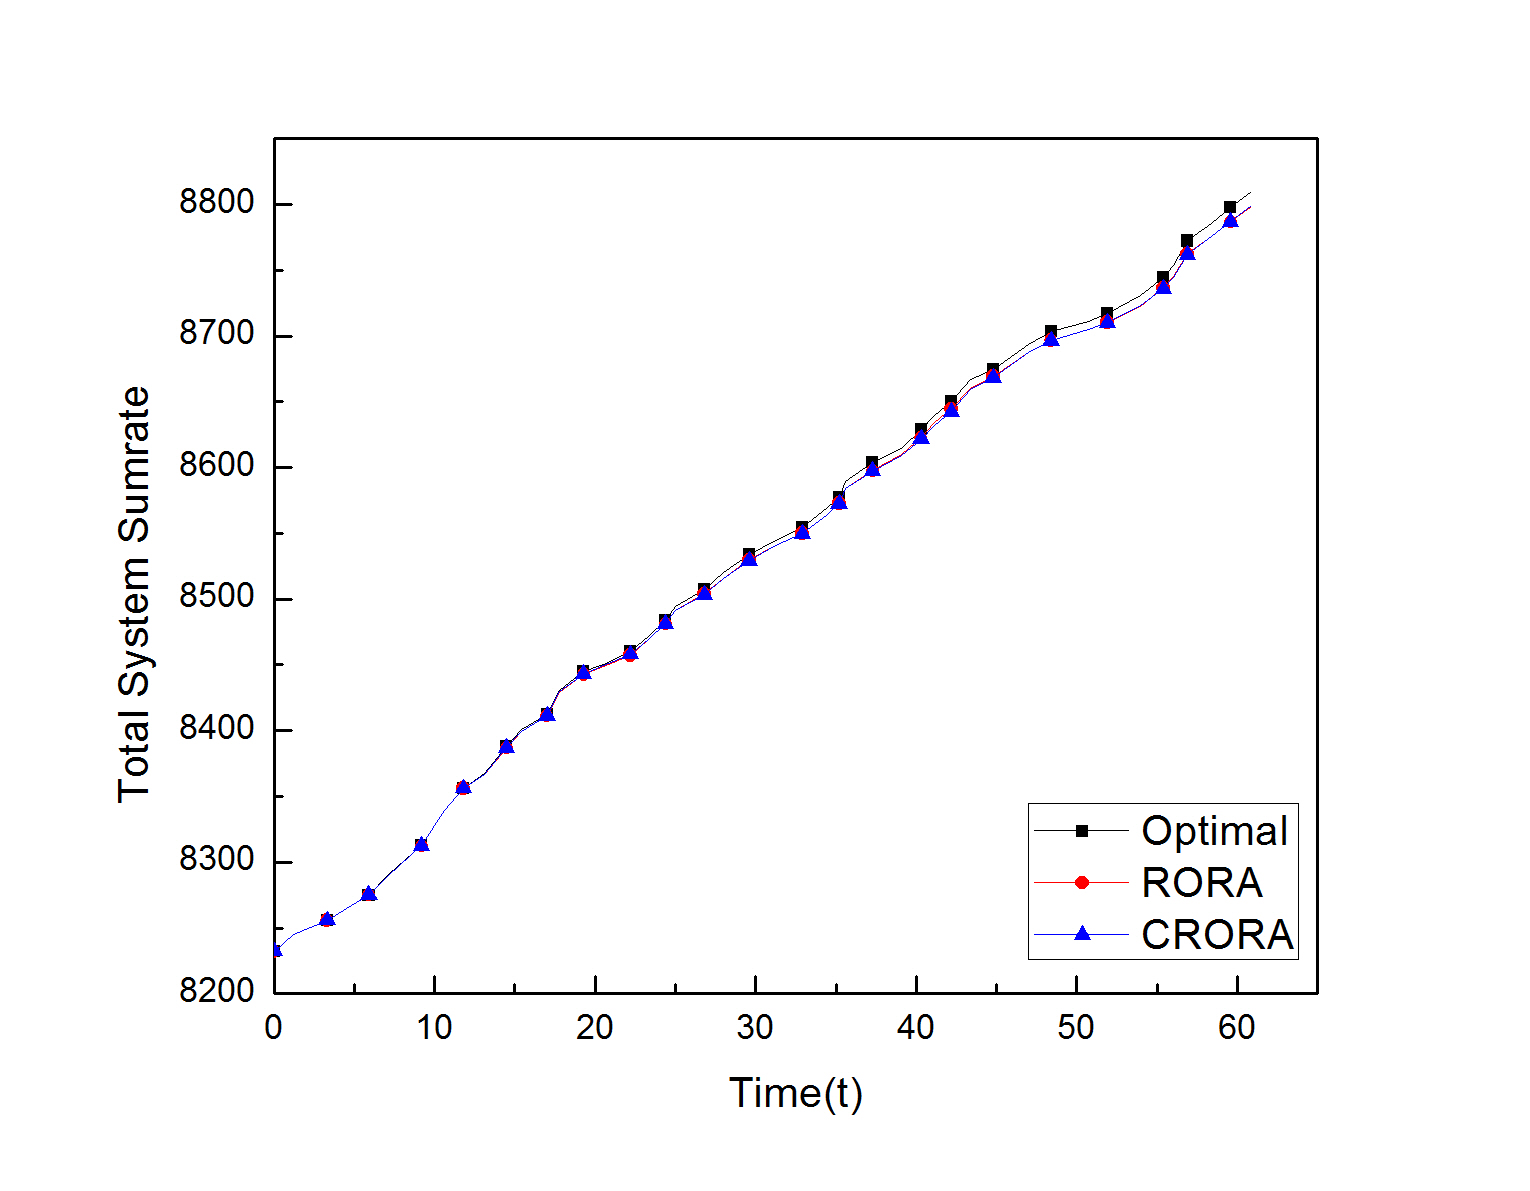
\includegraphics[width=90mm,height=60mm]{Graph/sumrateresjournal.jpg}
		\vspace{-0.2cm}
		\caption{Total System Sumrate in Each State of the System for the Restricted Assignment Scheme}
		\vspace{-.5cm}
		\label{fig:sum_r}
	}
\end{figure}



\begin{figure}[t]
	{ %
		\setlength{\fboxsep}{1.5pt}%
		\setlength{\fboxrule}{1.5pt}%
		\centering
		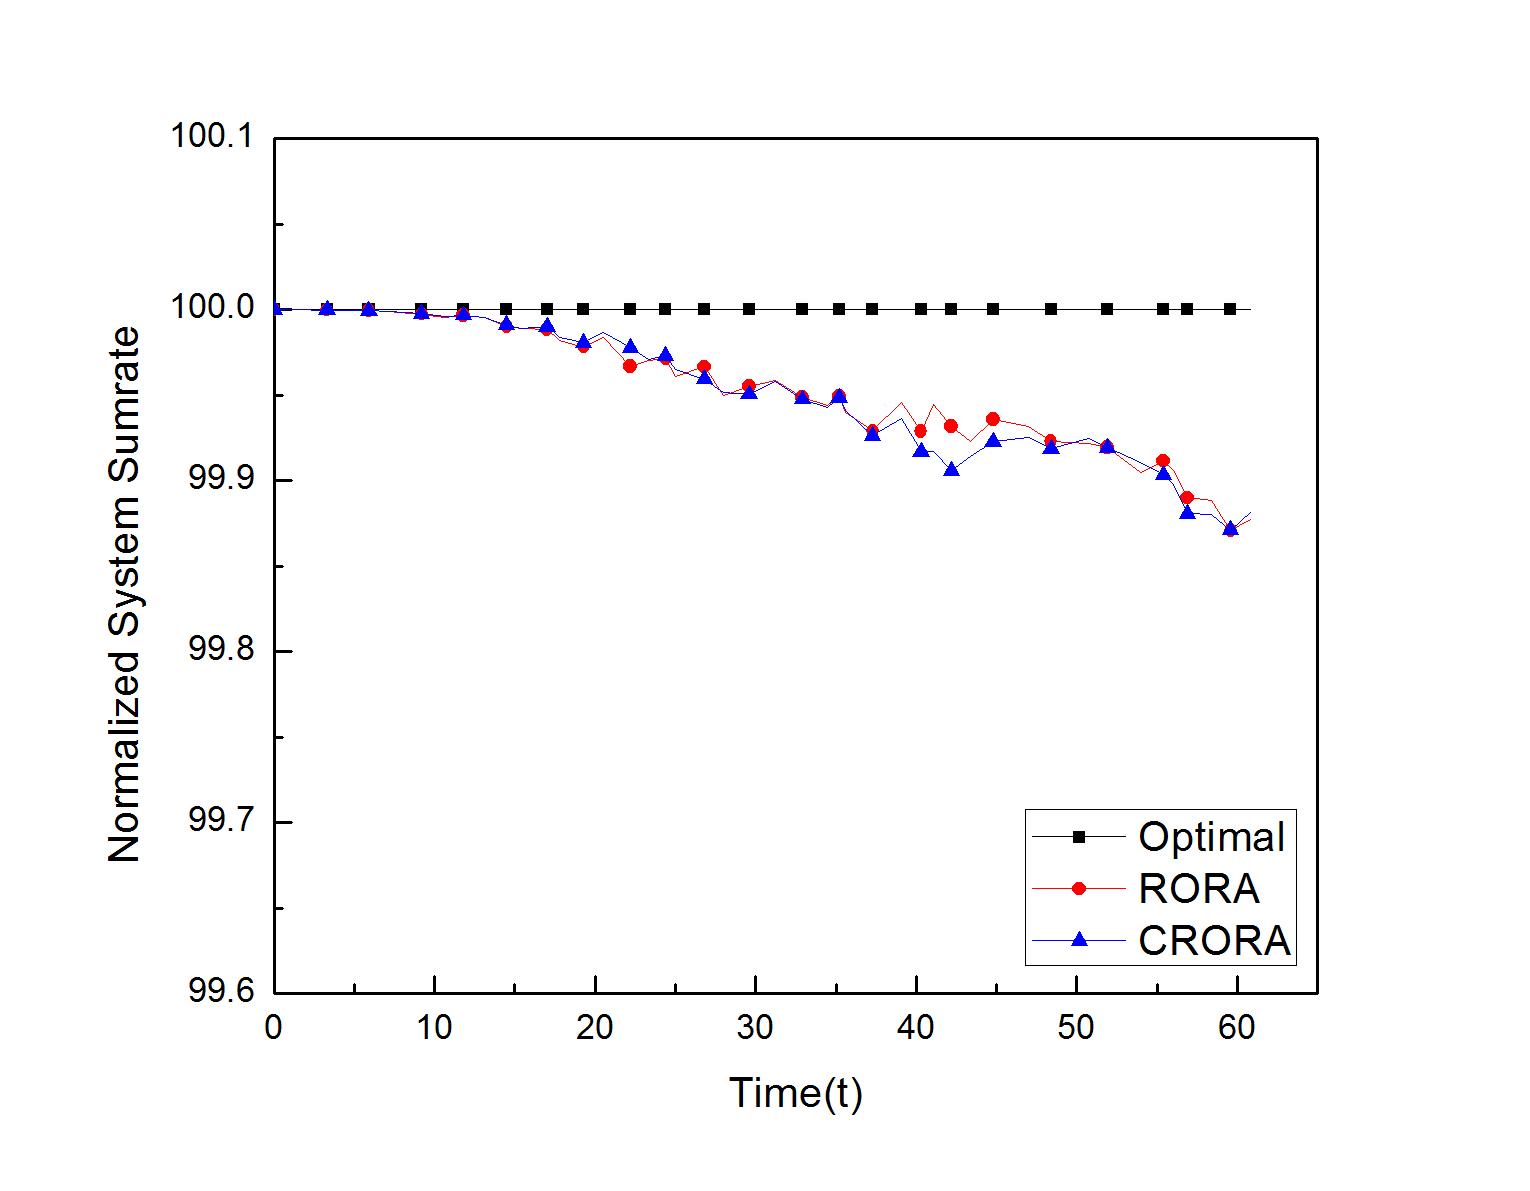
\includegraphics[width=90mm,height=60mm]{Graph/Normalizedsumrateresjournal.jpg}
		\vspace{-0.2cm}
		\caption{Normalized System Sumrate in Each State of the System for the Restricted Assignment Scheme (Normalized with Respect to the Optimal Hungarian Algorithm)} \label{fig:sum_r_N}
	}
	\vspace{-.5cm}
\end{figure}

\begin{figure}[t]
	{ %
		\setlength{\fboxsep}{1.5pt}%
		\setlength{\fboxrule}{1.5pt}%
		\centering
		%\vspace{-.5cm}
		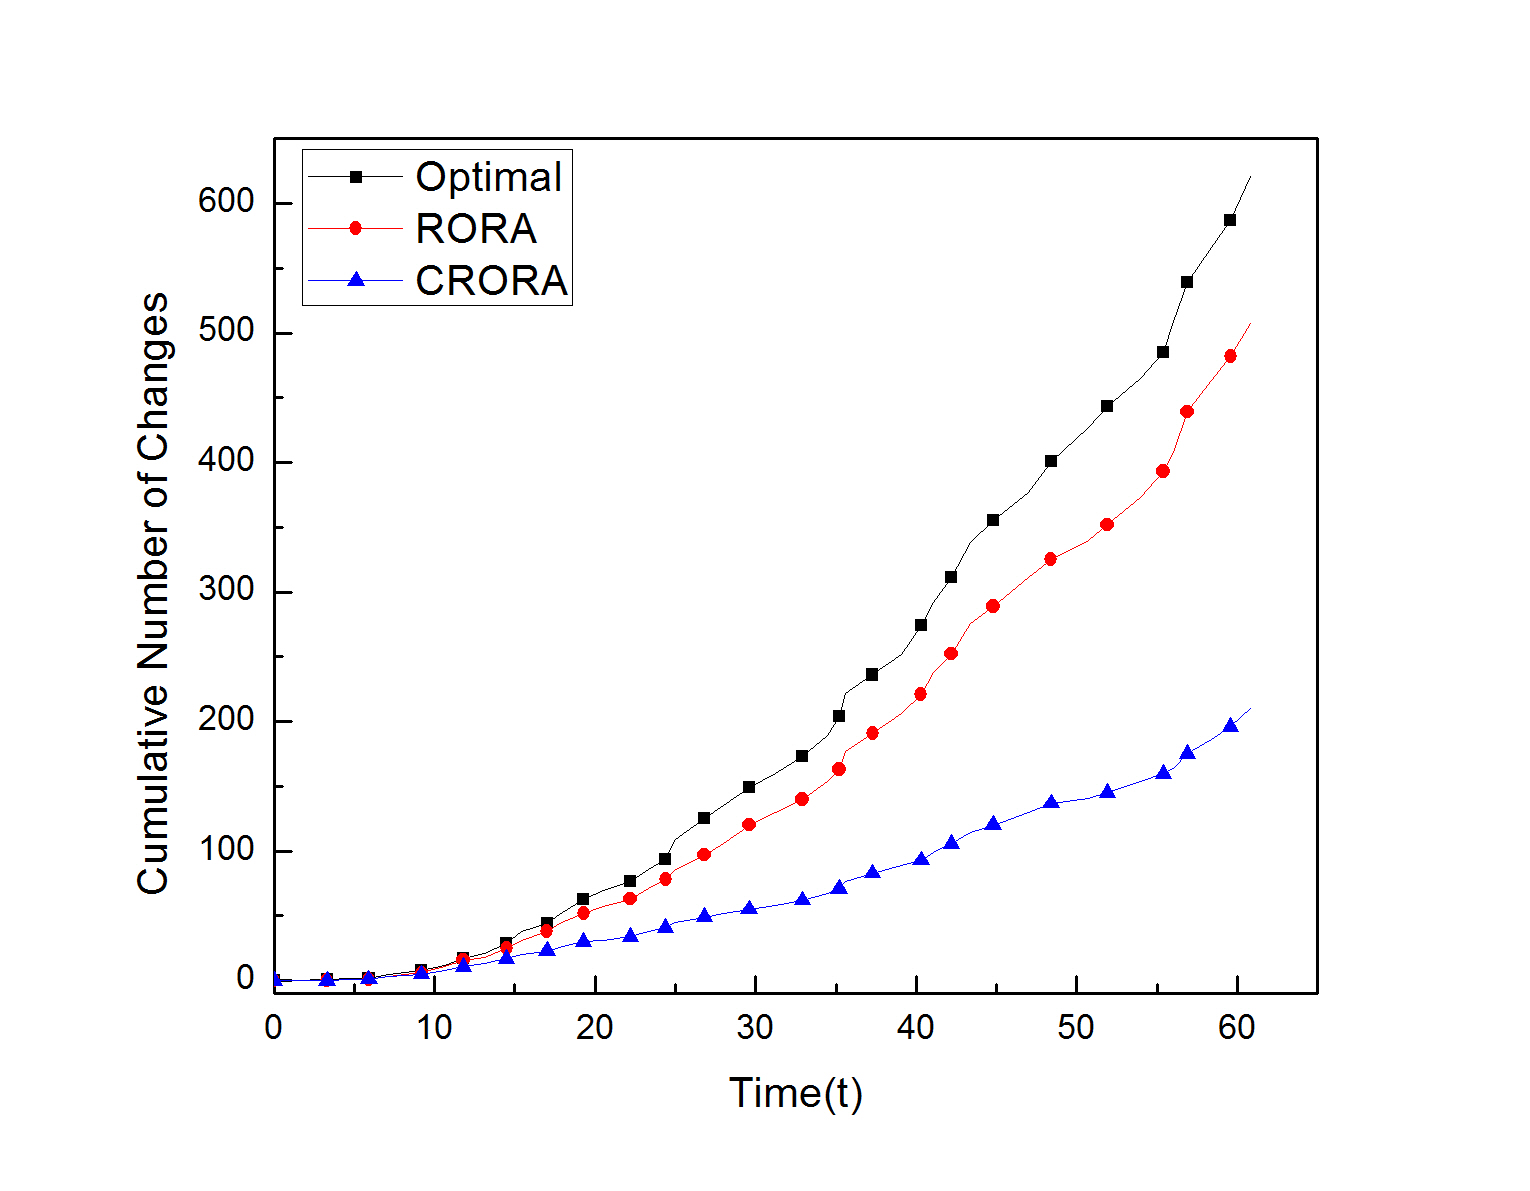
\includegraphics[width=90mm,height=60mm]{Graph/nocresJournal.jpg}
		\vspace{-0.2cm}
		\caption{Cumulative Number of Changes in Each State of the System for the Restricted Assignment Scheme} \label{fig:noc_r}
		\vspace{-.5cm}
	}
\end{figure}


\smallskip
\noindent
For the restricted assignment scheme, we compare RORA and CRORA with the optimal Hungarian algorithm only as there is no existing variant of the restricted version. Figure \ref{fig:sum_r} shows the comparison of the algorithms in term of the total system sumrate where individual line represents the increase of the total system sumrate returned by the algorithms with respect to time. Like the fair assignment scheme in the restricted assignment scheme, RORA and CRORA perform very near to the optimal (Hungarian) algorithm. For better visualization, we present the normalized system sumrate returned by different algorithms in the restricted assignment scheme in Figure \ref{fig:sum_r_N} where the graph is normalized with respect to the optimal algorithm. From Figure \ref{fig:sum_r_N} we can easily observe that in the restricted assignment scheme the performance of RORA and CRORA is almost similar which is approximately $99.97\%$ of the optimal Hungarian algorithm. Figure  \ref{fig:noc_r} represents the comparison of the algorithms in the restricted assignment scheme in term of the number of changes in assignment between two successive states. In the restricted assignment scheme RORA outperforms the optimal algorithm by performing approximately $20\%$ less number of changes in assignment between two successive allocations. On the other hand,  CRORA outperforms both RORA and the optimal algorithm where CRORA performs  approximately $60\%$ less number of changes than CRORA and approximately 68\% less number of changes than the optimal algorithm. We need to mention that, in the restricted assignment scheme, presumably some D2D pairs cannot be assigned those provide negative sumrate gain. The number of assigned D2D pairs by the optimal algorithm is $153$ out of a total of $225$ D2D pairs whereas RORA assigns $150$ D2D pairs and CRORA assigns $155$ D2D pairs out of $225$ D2D pairs finally present in the system.  

\smallskip
\noindent
Based on all of the simulation results we can say that in both of the assignment schemes our proposed algorithms (RORA and CRORA) return a total system sumrate that is very close to the total system sumrate returned by the optimal algorithm. Moreover, in the fair assignment scheme, RORA and CRORA outperform LORA and DARA in term of total system sumrate. On the other hand, in term of the number of changes both RORA and CRORA outperforms all of the algorithms in both of the assignment schemes.
\vspace {-0.3cm}
\section{Conclusion}\label{section:Conclusion}
\vspace {-0.3cm}
\smallskip
\noindent
D2D communication in underlay inband mode is the most beneficial as sharing the radio resources of existing cellular users with the D2D pairs increases the system capacity. This mode of personal communication is attracting more researchers from academia, standardization bodies, and industry for further insight and a lot more research is still necessary to achieve power and spectral efficiency by developing more efficient resource allocation schemes. This paper addresses the research problem of maximizing the system sumrate by sharing the RBs among the cellular UEs and the D2D pairs while maintaining the QoS. To the best of our knowledge, most of the existing research works in this area deal with offline resource allocation algorithms. The addressed research problem can be solved optimally in polynomial time using the weighted bipartite matching algorithm. However, in LTE and beyond (4G and 5G) systems, scheduling algorithms should be very efficient where the optimal algorithm is quite complex to implement. Hence, a low complexity algorithm which returns almost the optimal solution can be an alternative to this research problem. In this paper, we propose two relax online resource allocation algorithms for D2D communication in inband underlay mode. Our proposed algorithms consider two assignment schemes namely the restricted assignment scheme and the fair assignment scheme. The restricted assignment scheme provides better system sumrate by avoiding the assignments those contribute negative sumrate gain. On the other hand, the fair assignment scheme assigns more D2D pairs than the restricted assignment scheme by sacrificing some system sumrate gain. Network providers may choose any one of the schemes based on their need. We have done extensive simulations to validate our algorithms. Simulation results suggest that our proposed algorithms outperform the existing offline algorithms in terms of both total system sumrate and number of changes in successive allocation. Moreover, our proposed algorithms perform very close to the optimal algorithm in terms of system sumrate with less number of changes in successive allocation. According to the definition of online stable matching algorithm, our current implementation considers the cellular UEs as a fixed set and D2D pairs as an adversary set. However, assuming both of the cellular UEs and the D2D pairs as adversary sets would be an interesting research problem. We plan to investigate this issue in our future work.
%\vspace {-0.1cm}

\bibliographystyle{plain}
\bibliography{bibfile}
\end{document}
